%% uctest.tex 11/3/94
%% Copyright (C) 1988-2004 Daniel Gildea, BBF, Ethan Munson.
%
% This work may be distributed and/or modified under the
% conditions of the LaTeX Project Public License, either version 1.3
% of this license or (at your option) any later version.
% The latest version of this license is in
%   http://www.latex-project.org/lppl.txt
% and version 1.3 or later is part of all distributions of LaTeX
% version 2003/12/01 or later.
%
% This work has the LPPL maintenance status "maintained".
% 
% The Current Maintainer of this work is Daniel Gildea.
%
% 2007/08/01
% LaTeX Package "ucr" is modified from LaTeX package "ucthesis."
% This modification is therefore under to the conditions of 
% the LaTeX Project Public License.
% Its formality is suitable for the dissertation of Universty of
% California, Riverside.
% This test document is for the convenience of all students of
% Universty of California, Riverside.
% Contact Charles Yang at chcyang@yahoo.com if you like.
% Charles Yang has nothing to do with the original author's sarcasm.
%
%%%%%%%%%%%%%%%%%%%%%%%%%%%%%%%%%%%%%%%%%%%%%%%%%%%%%%%%%%%%%%%%%%%%%%%%%%%%%%%%%
%% Document: Thesis for PhD at UC Riverside                                    %%
%% Title: Investigating the evolution of environmental and biotic interactions %% 
%%          in basal fungal lineages through comparative genomics              %%
%% Author: Steven Ahrendt                                                      %%
%%%%%%%%%%%%%%%%%%%%%%%%%%%%%%%%%%%%%%%%%%%%%%%%%%%%%%%%%%%%%%%%%%%%%%%%%%%%%%%%%
% \documentclass[11pt]{ucthesis}
\documentclass[11pt]{UCR_latex_template/ucr}
%\documentclass[oneside,final,letter]{ucr}
\usepackage{anysize}
\usepackage[left=1.5in,top=1.5in,right=1in,bottom=1in]{geometry}
% \usepackage{bm}
% \usepackage{mathrsfs}
% \usepackage[dvips]{graphicx}
% \usepackage{graphics}
% \usepackage{subfigure}
% \usepackage{flafter}
% \usepackage{sw20uctd}
\usepackage{xspace}
\usepackage{graphicx}
\usepackage{Styles/pdfsync}
\usepackage{amsmath}
% \usepackage{amssymb}
% \usepackage{amsthm}
% \usepackage{fancyhdr} 
\usepackage{fncylab}
\usepackage[usenames]{color}
% \usepackage{enumerate}
% \usepackage{multirow}
% \usepackage{setspace}

%%---------------
%% Packages added by Steven Ahrendt
%%-----------//
%\usepackage{hyperref} % use for clickable links
\usepackage{url} % use with \url{} for formatted urls; nonclickable
\usepackage[graphicx]{realboxes}
\usepackage{texshade}
\usepackage{longtable}
\usepackage{booktabs}  % Added to make
%\usepackage{array}     %  tables look nice
%\usepackage{tabularx}  %
\makeatletter
\g@addto@macro\@floatboxreset\centering
\makeatother
\usepackage{lscape}
\usepackage{multirow}
\usepackage[english]{babel}      % for proper formatting of 
\usepackage[autostyle]{csquotes} % quotemarks
\usepackage{fancyvrb} % for including fasta file with \VerbatimInput
%%-------------------------------------//

\setcounter{secnumdepth}{3}
\setcounter{tocdepth}{3}

%\newtheorem{theorem}{Theorem}
%\newtheorem{acknowledgement}[theorem]{Acknowledgement}
%\newtheorem{algorithm}[theorem]{Algorithm}
%\newtheorem{axiom}[theorem]{Axiom}
%\newtheorem{case}[theorem]{Case}
%\newtheorem{claim}[theorem]{Claim}
%\newtheorem{conclusion}[theorem]{Conclusion}
%\newtheorem{condition}[theorem]{Condition}
%\newtheorem{conjecture}[theorem]{Conjecture}
%\newtheorem{corollary}[theorem]{Corollary}
%\newtheorem{criterion}[theorem]{Criterion}
%\newtheorem{definition}[theorem]{Definition}
%\newtheorem{example}[theorem]{Example}
%\newtheorem{exercise}[theorem]{Exercise}
%\newtheorem{lemma}[theorem]{Lemma}
%\newtheorem{notation}[theorem]{Notation}
%\newtheorem{problem}[theorem]{Problem}
%\newtheorem{proposition}[theorem]{Proposition}
%\newtheorem{remark}[theorem]{Remark}
%\newtheorem{solution}[theorem]{Solution}
%\newtheorem{summary}[theorem]{Summary}
%\newtheorem{observation}[theorem]{Observation}
\newenvironment{proof}[1][Proof]{\textbf{#1.} }{\ \rule{0.5em}{0.5em}}
\def\dsp{\def\baselinestretch{2.0}\large\normalsize}
\dsp

%TCIDATA{OutputFilter=LATEX.DLL}
%TCIDATA{Created=Saturday, April 29, 2006 22:07:22}
%TCIDATA{LastRevised=Tuesday, July 17, 2007 22:48:56}
%TCIDATA{<META NAME="GraphicsSave" CONTENT="32">}
%TCIDATA{<META NAME="DocumentShell" CONTENT="Other Documents\SW\Thesis - University of California Thesis">}
%TCIDATA{Language=American English}
%TCIDATA{CSTFile=ucr.cst}


%% tcilatex is a package from Scientific Workplace.
%% The user may remove the following line without serious damage.
%% \input{tcilatex}


\usepackage{Sweave}
\begin{document}
%%%%%%%%%%%%%%
% TITLE PAGE %
%%%%%%%%%%%%%%

% Declarations for Front Matter

\title{Investigating the Evolution of Environmental and Biotic Interactions in Basal Fungal Lineages Through Comparative Genomics}
\author{Steven Robert Ahrendt}
\degreemonth{August}
\degreeyear{2015}
\degree{Doctor of Philosophy}
\chair{Dr. Jason E. Stajich }
\othermembers{Dr. Chia-en A. Chang\\
Dr. Katherine A. Borkovich}
\numberofmembers{3}
\field{Genetics, Genomics, and Bioinformatics}
\campus{Riverside}

\maketitle
\copyrightpage{}
\approvalpage{}

\degreesemester{Summer}

\begin{frontmatter}
%%%%%%%%%%%%%%%%%%%%
% ACKNOWLEDGEMENTS %
%%%%%%%%%%%%%%%%%%%%
\begin{acknowledgements}
There are many people to whom I am deeply indebted for their contribution to this dissertation and to whom I would like to extend my appreciation. First and foremost, to my research advisor and mentor Dr. Jason Stajich, who allowed me both the freedom and guidance necessary to see this research to completion. To my co-advisor, Dr. Chia-en Angelina Chang, whose input and assistance helped provide a fresh perspective on aspects of this research. And to Dr. Katherine Borkovich, for her support, guidance, and technical expertise. To my undergraduate internship research advisor Dr. Jamie Foster at the Kennedy Space Center and her graduate student Jen, without whose inspiration, advice, and continued support I would never have pursued graduate school at all. I would like to extend a huge thank you to the members of the Stajich and Chang labs, and especially to the undergraduate students I mentored for their assistance; also to the members of the Borkovich lab, whose equipment and expertise I borrowed early and often. To my parents, for their constant support and continued patience. And finally to Kat, who joined me on the journey and stayed with me until the end, for which I am eternally grateful.\\
\indent The text of this dissertation, in part or in full, is a reprint of the material as is appears in \enquote{Shared Signatures of Parasitism and Phylogenomics Unite Cryptomycota and Microsporidia}, \emph{Current Biology}, 2013.  The co-author, Dr. Jason Stajich, listed in that publication directed and supervised the research which forms the basis for this dissertation.\\
% Funding provided by the University of California, Riverside, and by the Alfred P. Sloan foundation.\\
\end{acknowledgements}

%%%%%%%%%%%%%%
% DEDICATION %
%%%%%%%%%%%%%%
%\begin{dedication}
%\null\vfil
%{\large
%\begin{center}
%For Ruby.
%\end{center}}
%\vfil\null
%\end{dedication}

%%%%%%%%%%%%%%%%%%%%%%%%%%%
% ABSTRACT                %
% Include in abstract.tex %
%%%%%%%%%%%%%%%%%%%%%%%%%%%
%%%%%%%%%%%%%%%%%%%%%%%%%%%%%%%%%%%%%%%%%%%%%%%%%%%%%%%%%%%%%%%%%%%%%%%%%%%%%%%%%
%% Document: Thesis for PhD at UC Riverside                                    %%
%% Title: Investigating the evolution of environmental and biotic interactions %%
%%          in basal fungal lineages through comparative genomics              %%
%% Author: Steven Ahrendt                                                      %%
%%%%%%%%%%%%%%%%%%%%%%%%%%%%%%%%%%%%%%%%%%%%%%%%%%%%%%%%%%%%%%%%%%%%%%%%%%%%%%%%%
% ABSTRACT %
%%%%%%%%%%%%
\begin{abstract}
Species belonging to the early diverging fungal lineages (Blastocladiomycota, Chytridiomycota, Cryptomycota, and Neocallimastigomycota) reproduce via motile zoospores and are found in both aquatic and terrestrial environments. These organisms are traditionally understudied, despite being active decomposers, parasites, and symbionts with other organisms in the ecosystem. This dissertation research uses a comparative genomics approach to answer questions about these fungi and their interactions with their environment and other fungi. Chapter~\ref{chap:HpInhibition} describes surprising observations regarding competitive and inhibitory behavior in one member of the Chytridiomycota. Chapters~\ref{chap:RhodStruct} and \ref{chap:RhodAux} examine the feasibility of rhodopsin-mediate photoreception in basal lineages using structural mechanics and genome-wide gain-loss analyses. Chapter~\ref{chap:ClatTranscriptome} provides a transcriptome analysis of one member of the genus \textit{Coelomomyces}, the only known entomopathic chytrid genus. Appendix~\ref{app:Flagella} briefly looks at gain-loss analysis of molecular aspects of the evolutionary transition from aquatic motile single cells to terrestrial multicellullar organisms.\\
\end{abstract}


%%%%%%%%%%%%%%%%%%%%%
% TABLE OF CONTENTS %
%%%%%%%%%%%%%%%%%%%%%
\tableofcontents
\listoffigures
\listoftables
\end{frontmatter}

% \part{First Part}


%%%%%%%%%%%%%%%%
% INTRODUCTION %
%%%%%%%%%%%%%%%%
%%%%%%%%%%%%%%%%%%%%%%%%%%%%%%%%%%%%%%%%%%%%%%%%%%%%%%%%%%%%%%%%%%%%%%%%%%%%%%%%%
%% Document: Thesis for PhD at UC Riverside                                    %%
%% Title: Investigating the evolution of environmental and biotic interactions %%
%%          in basal fungal lineages through comparative genomics              %%
%% Author: Steven Ahrendt                                                      %%
%%%%%%%%%%%%%%%%%%%%%%%%%%%%%%%%%%%%%%%%%%%%%%%%%%%%%%%%%%%%%%%%%%%%%%%%%%%%%%%%%
% INTRODUCTION %
%%%%%%%%%%%%%%%%
\chapter{Introduction to the Basal Fungal lineages}
\section{Overview of fungal phylogenetics and the importance of the basal lineages}
%%%%%
% Fungal phylogenetics
%%%%%
The Fungi are one of the major kingdoms of eukaryotic life on Earth. Various studies have attempted to estimate the date of the emergence of the Kingdom Fungi \cite{Taylor2006}, when it diverged from the metazoan lineages. These studies place this occurance at approximately 1 billion years ago, with a range of around $\pm$500 MYA: 600 MYA \cite{Berbee1993}, 965 MYA \cite{Doolittle1996}, and 1.6 BYA \cite{Wang1999}. These loose approximations are based on correlation between evolutionary events in fungi and in other organisms, and are under continued re-evaluation and refinement \cite{Berbee2010}.\\
\indent A comprehensive review of a collection of 21st century phylogenetic studies \cite{Hibbett2007} proposes that the Fungal Kingdom comprises seven phyla: Microsporidia, Chytridiomycota, Blastocladiomycota, Neocallimastigomycota, Glomeromycota, Basidiomycota, and Ascomycota, with the most recent inclusion of the phylum Cryptomycota \cite{Jones2011}.\\
\indent The most recently diverged fungal phyla are the Ascomycota and Basidiomycota, and together make up the subkingdom Dikarya. This subkingdom is so named because its members undergo cell fusion (plasmogamy) without nuclear fusion (karyogamy) during sexual development, resulting in cells with nuclei from individual parents ("dikaryons"). These organisms are muticellular, with terrestrial habitats, sexual and asexual life cycle components, and filamentous growth structures. Collectively, the Dikarya is the most widely studied group and is home to several model and non-model organisms of research interest, including the model filamentous Ascomycete \textit{Neurospora crassa}, the economically critical \textit{Saccharomyces cerevisiae}, and the numerous medically relevant \textit{Aspergillus} spp.\\
\indent Going further back in time is the phylum Glomeromycota. This group contains mycorrhizal fungi (arbuscular and ento-) which associate with approximately 90\% of all plant species and are thus of greate ecological importance. This phylum also contains four subphyla \textit{incertae sedis}: Mucormycotina, Entomophthoromycotina, Zoopagomcotina, and Kickxellomycotina \cite{White2006}. These subphyla were previously classified in the phylum Zygomycota and contain primarily terrestrial fungi of various medical and industrial research interest. It is important to point out here that the definitive phylogenetic relationship between the Glomeromycota and Zygomycota \textit{incertae sedis} lineages is unresolved and is a current focus of research \cite{Hibbett2007}. Therefore in this text, the nonflagellated members of the Glomeromycota, Mucormycotina, Entomophthoromycotina, Zoopagomycotina, and Kickxellomycotina will, for convenience, be referred to collectively as Zygomycota.\\ 
\indent Closest to the fungal-animal evolutionary divergence are the basal fungal lineages: the Microsporidia, Cryptomycota, Chytridiomycota, Blastocladiomycota, and Neocallimastigomycota. It is these lineages, particularly the Blastocladiomycota and Chytridiomycota, on which this dissertation will primarily be regarding. These groups are sometimes collectively referred to as "chytrids", although this is not to be confused with the formal phylum Chytridiomycota. Broadly speaking, these organisms have asexual life cycles which progress through development as motile, flagellated zoospores, followed by sessile, non-flagellated, spore-producing sporangia. During the motile stage, the zoospore seeks an appropriate environmental substrate, encysts upon it, retracts its flagellum, and develops a cell wall. Many species will stay dormant in this stage as a thick-walled "resting spore", and only develop into a thin-walled zoosporangia after a certain time period \cite{James2006Blasto}. Other chytrid species will instead progress directly to the zoosporangia stage, undergo several rounds of mitotic cell division, and ultimately produces and releases hundreds of new zoospores \cite{James2006Blasto}. \\
\indent While generally being described as asexual, certain species within the Blastocladiomycota, such as \textit{Allomyces reticulatus} and \textit{Coelomomyces punctatus}, have demonstrated sexual reproductive cycles utilizing zoospores of different mating types \cite{Alexopoulos1996}.\\
%%%%%
% Importance of EDF
%%%%%
\indent The basal fungal lineages are characterized as true Fungi and distinct from other water molds, like Oomycetes, and fall sister to both Metazoan lineages as well as the other fungal lineages (Zygomycota, Ascomycota, and Basidiomycota). While these lineages only represent less than 2\% of all described fungi \cite{Stajich2009}, they serve as a unique system in which to infer characteristics presumed to have been present in the fungal-animal common ancestor.\\
\indent Additionally, basal fungal lineages are presumed to have a nearly cosmopolitan distribution \cite{Powell1993}. Members of these lineages fulfill nearly all varieties of ecological niches, primarily decomposition in terrestrial and aquatic environments, but also including pathogenic interactions with a wide variety of hosts: arbuscular mycorrhizal fungi (\textit{Spizellomyces punctatum} (Chytridiomycota) \cite{Paulitz1984}), insects (\textit{Coelomomyces psorophorae} (Blastocladiomycota) \cite{Zebold1979}), plants (\textit{Olpidium brassicae} (Chytridiomycota) \cite{Tewari1983}), vertebrates (\textit{Batrachochytrium dendrobatidis} (Chytridiomycota) \cite{Longcore1999}), nematodes (\textit{Catenaria anguillulae} (Blastocladiomycota) \cite{Deacon1997}) and algae (\textit{Zygorhizidium plantonicum} \cite{Canter1967}), and even to intracellular symbioses with other chytrids (\textit{Rozella allomyces} (Cryptomycota) \cite{Held1973}). This distribution of life styles speaks to the vast biological challenges they must face and therefore suggests a number of novel mechanisms which have yet to be fully studied and explored. \\
\indent Attempts at formal description of early-diverging fungi, based primarily on collection and observation, began as early as 1858 and proceeded through the latter half of 19th century with pioneering work of researchers such as Schroter, Fischer, Zopf, Lowenthal, Nowakowski, and Woronin \cite{Fitzpatrick1930}. A primarily systematic approach allowed for the establishment of (among others) the order Chytridiales, defined broadly as lacking mycelium and having an unknown sexual cycle, and the order Blastocladiales, defined as having mycelium and a sexual reproductive component.\\
\indent Revisions of fungal phylogenetics continued through the 20th century and included Alexopolous's series on Introductory Mycology in the 1950s.\\
\indent Significant microscopy work was carried out on chytrid species as early as 1953 by Koch and others, which allowed for the discussion of zoosporic ultrastructure characters. In the 1970s, the then recent technology of electron microscopy allowed for finer grain examinations of chytrid ultrastructure.\\
\indent In 1993, Mims and Blackwell for fourth edition (1996) using DNA-based phylogentics (specifically SSU rDNA). Importantly, established Fungi as monophyletic, established chytrids as Fungi, and excluded other heterokont flagellates (eg oomycetes).\\
\indent In 1999, James et al attempted to reconcile the previous ultrastructure-based phylogeny (using characters such as zoospore discharge, thallus development, ultrastructural features) with modern molecular techniques (eg ssu rDNA) used in assessing phylogentic relationships in other fungal groups.\\
\indent It was around that time that the Chytridiomycete \textit{Batrachochytrium dendrobatidis} emerged as a global pathogen and the accepted causative agent of worldwide amphibian decline \cite{Berger1998}.\\
\indent By 2006, at the time of the establishment of the Deep Hypha coordination network, the Chytridiomycota was accepted as one of the four major fungal phyla (alongside the Zygomycota, Basidiomycota, and Ascomycota).\\
\indent Despite widespread distribution in both geography and ecology, chytrids remain understudied as a whole, driven in part because few species are of substantial economic importance \cite{Powell1993,James2000} as well as moderate difficulty in collection and culturing methods. \\
%%%%%
% Chytrid Bioinformatic resources 
%%%%%
\section{History of bioinformatic resources for basal fungi}
As whole genome sequencing continues to become more widely accesible, chytrid genomes are more easily developed. The first available bioinformatic resource was an expressed sequence tag (EST) dataset published in 2005 for the Blastocladiomycete \textit{Blastocladiella emersonii} \cite{Ribichich2005}. This collection of 16,984 high-quality ESTs provided a first approach to understanding gene complexity in chytrids. In 2006, a draft assembly for the genome of \textit{B. dendrobatidis} strain JEL423 was made publically available through the Broad Institute Fungal Genome Initiative (http://www.broadinstitute.org/). The resulting assembly is 23.72 Mb, represents 7.4X coverage of this diploid strain, and was the first whole genome assembly for any chytrid. In 2008, a second draft genome was released for \textit{B. dendrobatidis} strain JAM81 through the Joint Genome Institute (http://genomeportal.jgi-psf.org/Batde5/Batde5.home.html). This assembly is 24.3 Mb and represents 8.74X coverage. \\
\indent As part of a push to understand the Origins of Multicellularity, the genomes for the \textit{Allomyces macrogynus} (Blastocladiomycete) and the exclusively terrestrial \textit{Spizellomyces punctatus} (Chytridiomycete) (24.1 Mb) were sequenced by the Broad Institute in 2009. \\
\indent In 2011, the non-pathogenic \textit{Homolaphlyctis polyrhiza} JEL142, the closest relative to \textit{Bd} was sequenced for comparision to try to identivy aspects of pathogenicity in \textit{Bd} \cite{Joneson2011}. The resulting assembly size was inferred at 26.7 Mb (haploid) and represented 11.2X coverage. In 2014, with the help of a postdoctoral researcher in the Stajich Lab, Dr. Peng Liu, I generated Illumina sequencing libraries for \textit{H. polyrhiza} and helped assess the assembly and annotation with Dr. Stajich; the results of which are described in Chapter~\ref{chap:HpInhibition}.\\
\indent \textit{Gonapodya prolifera} (Monoblepharidomycota) is an aquatic fungus with both sexual and asexual reproductive schemes, and encompassing both hyphal and zoosporic growth stages. In the environment, \textit{G. prolifera} is an active degrader of plant material \cite{Karling1977}. A draft genome assembly was published in 2011 through JGI, with the goal of identifying potentially novel degredation-related enzymes for biofuels applications.\\
\indent \textit{Catenaria anguillulae} (Blastocladiomycota) is a facultative parasite of nematodes \cite{Deacon1997}. A draft genome was published in 2010 by the JGI and represented the second Blastocladiomycete genome (after \textit{A. macrogynus}). Genomic resources for \textit{C. anguillulae} would allow for research into monitoring and potential remediation strategies as the nematodes upon which it parasitizes are themselves parasites of agriculturally important crops.\\
\indent Members of the Neocallimastigomycota lineage, first isolated and described in 1975, are found in the anaerobic environment of mammalian rumen \cite{Orpin1975}. These fungi are uniquely adapted to degradation of the high fiber content of the typical diets of cattle and sheep. Thus they are important models for potential manipulation to not only improve digestion in these livestock sources \cite{Ho1995} but also potential biofuels applications \cite{Youssef2013}. \textit{Piromyces} and \textit{Orpinomyces} are two members of this group and were sequenced in 2011 and 2013, respectively, in the hopes that understanding the genomic content would provide starting points for these applications. \\
\indent The genome of Cryptomycete \textit{Rozella allomycis}, the intracellular parasite of \textit{Allomyces}, was sequenced in 2013 \cite{James2013} and the analysis used to propose a unification of the Cryptomycota and Microsporidian lineages.\\
\indent In 2014 the first transcriptome of the mosquito pathogen \textit{Coelomomyces lativitattus} (\textit{Cl}) was generated by isolating RNA from gametes emerging from copepods. The RNA extraction and Illumina library preparation was performed by Rob Hice, a reasercher in Dr. Brian Federici's lab at UCR. The sequencing was performed at the UCR IIGB Genomics core. The resulting sequence data was assembled and annotated using scripts provided by Dr. Jason Stajich, and my analysis is described in Chapter~\ref{chap:ClatTranscriptome}.\\
\indent The near future of bioinformatics resources for the basal lineages is promising due to the efforts of the 1000 Fungal Genome Project (http://1000.fungalgenomes.org) with plans to sequence at additional chytrid fungi, including \textit{Operculomyces laminatus} JEL223, \textit{Rhizoclosmatium hyalinus} JEL800, and \textit{Obelidium mucronatum} JEL802. \\
%%%%%
% Research goals
%%%%%
\section{Hypotheses and Objectives}
\indent Rapid advances in the feasability of genome sequencing have yielded and will continue to yield an increasing number of fungal genomes, especially those in the early-diverging lineages, for comparative analyses. While incorporating comparisons to already well-characterized representative fungal groups, this dissertation work gives specific focus to members of the early-diverging lineages, and in particular to the ones for which genomic resources are available and which have obvious economic or ecological importance: the amphibian pathogen \textit{Batrachochytrium dendrobatidis} and its closest, non-pathogenic relative, \textit{Homolaphlyctis polyrhiza}; the saprobic \textit{Spizellomyces punctatus}; and the aquatic Blastocladiomycete \textit{Allomyces macrogynus} and related \textit{Catenaria anguillulae}. This thesis is presented in four chapters comprising three aspects of biology focused on sensing and interpretation of biotic and environmental signals.\\
\subsection*{Competition-based secondary metabolism and anti-fungal properties of \textit{Homolaphlyctis polyrhiza}}
Interactions between microorganisms are facilitated by biological signals. These include proteins, small molecules, and various chemical compounds, either bound to the cell surface or secreted into the environment. Many of these compounds can be classified as secondary metabolites: chemicals not required for growth or development of the organism.\\
\indent Resource competition likely plays a role in the evolution of natural antifungal production \cite{Vicente2003}. Secretion by an organism in a resource-limited environment of secondary metabolites which also happen to negatively impact neighboring organisms would confer a selective advantage upon the producer. \\
\indent Comparative genomic analyses have identified a host of degradation enzymes in basal fungi, suggesting saprotrophic and sometimes pathogenic associations with other organisms. There are few explored examples of secreted or secondary metabolite molecules produced by any of the zoosporic fungi.\\ 
\indent Secondary metabolite production as it applies to basal fungi is discussed in more detail in Chapter~\ref{chap:HpInhibition} using the non-pathogenic Chytridiomycete \textit{Homolaphlyctis polyrhiza} JEL142. In this chapter, I address three major questions regarding an initial observation I made in the Stajich lab of \textit{Hp} inhibition of the vegetative hyphal growth of \textit{N. crassa} via an unknown secreted compound. Namely, "Is Hp unique among the chytrids in this behavior?", "Is this behavior specific to \textit{N. crassa}?", and "What is the underlying biochemical mechanism by which this behavior is accomplished?". These questions are addressed using observational assays with the sporangia of related Chytridiomycetes, and probing the breadth of non-Chytridiomycete fungi whose growth is susceptible to \textit{Hp}, encompassing Ascomycete, Basidiomycete, and Zygomycete species, and including both temperature and proteinase screens. Finally, to better explore \textit{Hp} gene content, I produced an improved genome assembly and annotation, by assisting Dr. Peng Liu and Dr. Jason Stajich in the collection of fungal material and the assembly and annotation of the resulting genome sequence.\\
\subsection*{Mechanics and evolution of Fungal rhodopsin-based photosensing in the basal lineages}
\indent During the course of a given day, an organism experiences a multitude of environmental stimuli, with light being one of the most prominent. The biochemical ability to appropriately process and respond to these signals is an incredibly complex and involved task, and understanding the underlying mechanisms of these responses is an ongoing scientific challenge. \\
\indent Previous work has shown that some of the basal fungi are phototaxic (see \cite{Saranak1997} and \cite{Muehlstein1987}), however the full extend of photosensing in zoosporic fungi has not been fully explored. A recent review of fungal photobiology suggests a sporadic distribution of photosensory proteins among the non-flagellated fungal lineages (ie Zygomycota and Dikarya), with little emphasis placed on the basal lineages \cite{Idnurm2010}. There are many classes of photoreceptor proteins in fungi capable of producing a cellular response from an environmental light signal, all of which have different mechanisms of action and specializations: phytochromes, cryptochromes, the white-collar complex, and opsins \cite{Idnurm2010}. In plants, phytochromes function as day-night sensors to regulate the circadian rhythm and flowering response. This is accomplished through a conformational shift between the red and far-red sensitive forms of the protein structure \cite{Rockwell2006}. While relatively little is known about fungal phytochrome function, research on A. nidulans suggests that the phytochrome protein is a member of an elaborate complex with regulatory functions involved with the asexual-sexual transition and secondary metabolite biosynthesis \cite{Idnurm2010}. Cryptochromes, found predominantly in plants, animals, and insects, are blue-light sensitive proteins involved in circadian rhythm regulation and light activated DNA damage repair \cite{Idnurm2010}. Additional evidence suggests cryptochrome proteins play a role in mediating the phototactic behavior of sponge larvae \cite{Rivera2012}.\\
\indent First studied in the model filamentous Ascomycete fungus \textit{Neurospora crassa}, the well-characterized white-collar complex assembles as a heterodimer comprising White-collar 1 and 2 proteins. This complex functions to sense blue and near UV wavelengths, and, when active, directly interacts with DNA to regulate the circadian clock machinery, sporulation, pigmentation, and phototropism \cite{Ballario1997,Purschwitz2006,Corrochano2007}. \\
\indent The largest family of membrane receptors by far is that of the seven-transmembrane (7TM) receptors, comprising upwards of 800 genes \cite{Pierce2002}. This family includes various receptors for a wide range of ligands, including hormones, neurotransmitters, odorants, and photons. While there are three distinct subfamilies (A, B, and C), they share very little sequence similarity. Opsins, examples of which can be found in bacteria, archaea, and eukaryotes, are part of the largest family of 7TM proteins. One subclass of opsin, the Type 2 rhodopsins, are G-protein-coupled receptor (GPCR) proteins which function via photoisomerization of a covalently bound retinyledene chromophore, typically 11-\textit{cis}-retinal \cite{Wald1968}.\\
\indent The retinal chromophore utilized in Type 2 rhodopsin-mediated photoreception is biosynthesized from $\beta$-carotene \cite{VonLintig2000}. Photoisomerization of this chromophore results in a conformational shift to the all-\textit{trans} isomer \cite{Smith2010} and activation of the coupled heterotrimeric G-protein. A comparative analysis of auxillary proteins in basal fungi involved in this downstream signalling cascade is given in Chapter~\ref{chap:RhodAux}, and a description of findings dealing with structural and functional analyses of putative homologs of Type 2 rhodopsin in several species of basal fungi is provided in Chapter~\ref{chap:RhodStruct}.\\
\indent Biosynthesis of $\beta$-carotene begins with phytoene cyclase converting two molecules of geranylgeranyl pyrophosphate to one molecule of phytoene. Phytoene desaturase then works in a five-step pathway to convert phytoene into lycopene \cite{Hausmann2000}. Lycopene cyclase finally acts to convert lycopene to $\beta$-carotene \cite{Cunningham1994}. Subsequently, two different cleavage enzymes can potentially act on $\beta$-carotene. The enzyme $\beta$,$\beta$-carotene 15,15'-monooxygenase 1 (BCMO1) cleaves $\beta$-carotene into two all-\textit{trans}-retinal molecules, and is considered a key enzyme for retinoid metabolism \cite{Lietz2012}. The structurally related enzyme $\beta$,$\beta$-carotene 9',10'-dioxygenase (BCDO2) also acts on $\beta$-carotene to produce $\beta$-apo-10'-carotenal and $\beta$-ionone, however its physiological role is less well-characterized \cite{Lobo2012}. Comparative analysis and discussion of retinal biosynthesis enzymes is provided in Chapter~\ref{chap:ClatTranscriptome}.\\
\subsection*{Towards the development of bioinformatic resources for entomopathogenic Blastocladiomycete \textit{Coelomomyces lativittatus}}
\begin{itemize}
  \item Fungi which invade insects have been observed since antiquity (900 AD in Japan)\\
  \item Exact nature of fungal-insect relationship was not cleanly determined until 1888\\
  \item Once that was established, research switched to application of agriculture pest contro (1895-1925)\\
  \item Interest waned (1925-1960), but taxonomic knowledge greatly increased
  \item renewed interest is ongoing
\end{itemize}
\indent Certain insect-associated fungi are pathogenic on mosquitos. Of these, members of the genus \textit{Coelomomyces} in the Blastocladiomycota are the only known chytrid entomopathogens. While initially studied as a promising avenue for mosquito control, and an alternative to traditional pesticides, difficulties in culturing \textit{Cl} have lead to a decline in its research. However its specific host range and continued search for pesticide alternatives have allowed it to persist as an interesting avenue of research.\\
\indent Chapter~\ref{chap:ClatTranscriptome} presents a preliminary analysis of transcriptome data obtained from \textit{Coelomomyces lativittatus}. This analysis serves two purposes. First, it lays the groundwork for future RNASeq and proteomic studies of this organism. And secondarily, it attempts to assign molecular detail to previously published observational research about certain biochemical mechanisms (eg $\beta$-carotene production and photoreception).\\
\subsection*{Eukaryotic Flagellar motility}
One of the defining characteristics of the early-diverging fungal lineages is the presence of a posterior flagellum, which is used by the zoospores for motility \cite{Koch1958}. The chytrid flagellar apparatus is composed of the flagellar stalk (axoneme), the kinetosome (basal body), and the rootlet system \cite{Barr1981}. Additionally the characteristic 9+2 arrangment characteristic in other eukaryotic flagellated organisms persists.\\
\indent During the course of fungal evolution, there was a transition from flagellated motile aquatic single celled organisms to terrestrial multicellular organisms \cite{Taylor2006}. There is support for anywhere from a single flagellar loss event \cite{Liu2006} to at least four different such events \cite{James2006sixGene} prior to the divergence of the Zygomycota.\\
\indent The chytrid flagellum is the primay method of zoospore motility. In most cases, the chytrid flagellum exists as a posteriorly oriented appendage, with a few exceptions. The zoospores of the Neocallimastigomycota lineages, species most commonly found in the anaerobic environment of the mammalian rumen, are posteriorly multiflagellated \cite{Ho1995}. In the Blastocladiomycota, \textit{Coelomomyces} species are biflagellate during a part of their life cycle after the uniflagellate gametes of opposing mating types fuse to form a biflagellate zygote \cite{Padua1986}.\\ 
\indent A short treatment of comparative genomics work on the chytrid flagellar apparatus is given in Appendix~\ref{app:Flagella}. Included is a collection of genes which serve as a "core chytrid" flagellar geneset, which may prove useful in future assessments of chytrid and other basal fungal genomes.\\


%%%%%%%%%%%%%%%%%%%%%%%%%%%%%%%%
% RHODOPSIN STRUCTURAL CHAPTER %
%%%%%%%%%%%%%%%%%%%%%%%%%%%%%%%%
%%%%%%%%%%%%%%%%%%%%%%%%%%%%%%%%%%%%%%%%%%%%%%%%%%%%%%%%%%%%%%%%%%%%%%%%%%%%%%%%%
%% Document: Thesis for PhD at UC Riverside                                    %%
%% Title: Investigating the evolution of environmental and biotic interactions %%
%%          in basal fungal lineages through comparative genomics              %%
%% Author: Steven Ahrendt                                                      %%
%%%%%%%%%%%%%%%%%%%%%%%%%%%%%%%%%%%%%%%%%%%%%%%%%%%%%%%%%%%%%%%%%%%%%%%%%%%%%%%%%
%% RHODOPSIN: STRUCTURAL CHAPTER %%
%%%%%%%%%%%%%%%%%%%%%%%%%%%%%%%%%%%
\chapter{Structural characteristics of opsin-like proteins found in basal fungal lineages}
\label{chap:RhodStruct}
%%%%%%%%%%%%%%%%%%
%% Introduction %%
%%%%%%%%%%%%%%%%%%
\section{Introduction}
During the course of a given day, an organism experiences a multitude of environmental stimuli, including chemicals, gravity, the Earth's magnetic field, pressure, and light. The biochemical ability to appropriately process and respond to these signals is an incredibly complex and involved task, and understanding the underlying mechanisms of these responses is an ongoing scientific challenge. \\
\indent The presence or absence of light is perhaps one of the easiest sources of stimuli to comprehend and observe. The sun and rotation of the planet has had such a profound influence on the development of life that it comes as no surprise to find some form of photoreception in every major lineage on the planet. The widespread occurrence of such an ability, however varied in its implementation, speaks to its importance during the earliest stages of development of life. \\
\indent In Fungi, there are several classes of proteins capable of photoreception, all of which have different mechanisms of action and specializations. These include phytochrome, cryptochrome, white-collar, and opsin \cite{Idnurm2010}. In plants, phytochromes function as day-night sensors to regulate the circadian rhythm and flowering response. This is accomplished through a conformational shift between the red and far-red sensitive forms of the protein structure \cite{Rockwell2006}. While relatively little is known about fungal phytochrome function, research on \textit{A. nidulans} suggests that the phytochrome protein is a member of an elaborate complex with regulatory functions involved with the asexual-sexual transition and secondary metabolite biosynthesis \cite{Idnurm2010}. The white-collar complex (WCC), on the other hand, is very well characterized in Fungi. First studied in the model filamentous Ascomycete fungus \textit{Neurospora crassa}, WCC functions as a heterodimer comprising White-collar 1 and 2 proteins to sense blue and near UV wavelengths, and, when active, directly interacts with DNA to regulate the circadian clock machinery, sporulation, pigmentation, and phototropism \cite{Ballario1997,Purschwitz2006,Corrochano2007}. Cryptochromes are photoreceptors which belong to a large group of flavoproteins. Initial observations of blue-light sensitive photoreception in plants, without concurrent description of the responsible photoreceptor protein, led to the name \enquote{cryptochrome}: because of their \enquote{cryptic} nature \cite{Cashmore1999}. These proteins can be found in plants, animals, and insects, and are involved with circadian rhythm regulation and light activated DNA damage repair \cite{Idnurm2010}.\\
\indent Rhodopsin is a broadly defined term used to describe a large class of seven-transmembrane proteins which use retinylidene compounds for photoreception. This class can be subdivided into two types based on sequence similarity and function, despite similarities in structure (ie seven helical transmembrane domains) and mechanism of activation (ie photoisomerization of a retinaldehyde chromophore) \cite{Spudich2000}.\\
\indent The ion transporter rhodopsins (\enquote{Type 1}) are activated by the photoisomerization of all-\textit{trans}-retinal to 13-\textit{cis}-retinal. These function as membrane channels and are typically used for light-driven membrane depolarization via proton or chloride ion pumping. Examples of this group can be found in bacteria, archaea, and eukaryotes, and include the bacterial sensory rhodopsins, channelrhodopsins, bacteriorhodopsins, halorhodopsins, and proteorhodopsins.\\
\indent The G-protein coupled receptor (GPCR) rhodopsins (\enquote{Type 2}) are activated by the photoisomerization of 11-\textit{cis}-retinal to all-\textit{trans}-retinal. These function as visual receptors, and are the largest class of an even larger GPCR superfamily found only in eukaryotes. The general class of photosensitive GPCRs in animals are often referred to as \enquote{opsins}, with the visual opsins being one of the distinct subfamilies and known as \enquote{rhodopsins}. In animals, the other subfamiles are the melanopsins, peropsins, neuropsins, and encephalopsins. The exact nature of the evolutionary relationship between the Type 1 and Type 2 rhodopsins has not been clearly established and is currently the subject of discussion \cite{Terakita2005,Shichida2009}.\\
\indent Nonetheless, the rhodopsin pigment of both types is generated when the retinaldehyde chromophore is covalently joined to an opsin apoprotein via a Schiff-base linkage to a conserved lysine residue. While 11-\textit{cis}-retinal is the most common chromophore observed in vertebrates and invertebrates, others are found elsewhere in nature. For example, 3,4-dehydroretinal is observed in fish, amphibia, and reptiles. Switching between the 11-\textit{cis} and 3,4-dehydro- chromophores can be employed as a light adaptation strategy in certain freshwater fish \cite{Shichida2009}. 3-hydroxyretinal is found in insects, while 4-hydroxyretinal is observed in the firefly squid. In addition to the 11-\textit{cis} conformation, retinal can adopt a number of different isomers, including all-\textit{trans}, 13-\textit{cis}, and 9-\textit{cis} \cite{Shichida2009}. Molecular mechanics simulations suggest that the 11-\textit{cis}-retinal isomer has been selected for evolutionarily as the optimal chromophore due to the energetic stability of the resulting chromophore-opsin construct \cite{Sekharan2011}.\\ 
\indent Previous work has demonstrated that certain basal fungal species are phototaxic. For example, the phototactic capabilities of the marine fungus \textit{Rhizophydium littoreum} were quantified in 1987. This fungus demonstrated responses to light at a variety of wavelenths, with the most rapid response occuring at 400 nm. While the evidence strongly suggests a blue-light sensitive photoreceptor, the researchers were unable to specifically characterize the active photoreceptor \cite{Muehlstein1987}.\\
\indent A decade later, Saranak and Foster described their work on the phototactic capabilities of the Blastocladiomycete \textit{Allomyces reticulatus} \cite{Saranak1997}. This fungus has a visible, red-pigmented eyespot in which the photosensitive proteins are localized. Careful analysis determined that action spectrum of the phototactic zoospores peaks at 536$\pm$ 4 nm, simlar to that of the human green-sensitive cone. Furthermore, the researchers were able to destroy and subsequently restore the phototactic phenotype by reversibly inhibiting the biosynthesis of $\beta$-carotene, the molecular precursor to retinal. Taken together, these results suggested the presence of a rhodopsin protein of the Type 2 subfamily.\\
\indent The increasing availability of genomes from the traditionally understudied basal fungal lineages, coupled with a fairly well understood and important environmental sensing system, yields an opportunity to expand on known information about the photosensory response in fungi. In this chapter, I describe a computational approach toward understanding the structural mechanisms involved with rhodopsin-specific photoreception in basal fungi.\\

%%%%%%%%%%%%%
%% Methods %%
%%%%%%%%%%%%%
\section{Methods}

%---- Homology modeling and docking ----%
\subsection*{Sequence identification and homology modeling}
Putative rhodopsin sequences in basal fungal lineages were identified based on sequence similarity to the Profile Hidden Markov model from the Pfam database \cite{Finn2014}, accession PF00001 (\enquote{7tm\_1}). Identified fungal sequences were aligned with a subset of animal rhodopsin sequences from GenBank using Expresso \cite{Armougom2006}, a modified version of T-Coffee \cite{Notredame2000}, which incorporates protein structural information to guide the sequence alignment. The MAFFT \cite{Katoh2002,Katoh2005} and Muscle \cite{Edgar2004} multiple alignment modules were added to the default Expresso alignment. Based on the multiple sequence alignment, the structure model of the \textit{B. dendrobatidis} protein was built using Modeller (v9.9) \cite{Eswar2007} with explicit loop refinement and refined with OPUSRota (v1.0) \cite{Lu2008}. The \textit{S. punctatus} and \textit{A. macrogynus} models were constructed using iTASSER against the provided GPCR specific library \cite{Zhang2008}. The \textit{Bd} sequence was initially modeled using iTASSER along with the \textit{Sp} and \textit{Am} sequences. However, the Modeller-produced model was selected for further analyses as a conserved structural motif in EL2 of the iTASSER best-scoring model for \textit{Bd} was modeled incorrectly when compared to crystal structures 2Z73 and 1U19, and the \textit{Sp} and \textit{Am} iTASSER models. For the \textit{Sp} model, manual correction of the K320 orientation was performed by energy minimization using the general Amber force field (GAFF) \cite{Wang2004} in Avogadro \cite{Hanwell2012} after automatic refinement with OpusROTA.\\ 
\indent For the structures generated using Modeller, the output consisted of five potential models and corresponding Discrete Optimized Protein Energy (\enquote{DOPE}) \cite{Shen2006} and MODELLER objective function (\enquote{molpdf}) scores. Optimal models were therefore selected which had the lowest DOPE and molpdf values. For the iTASSER structures, the optimal model was selected using the iTASSER provided \enquote{c-score}, a confidence value based on the significance of threading template alignments.\\
\indent The quality of these selected models was assessesd using PROCHECK (v3.5) \cite{Laskowski1993,Wiederstein2007} and Verify3D \cite{Luthy1992}. The melatonin model was constructed using the human melatonin sequence (UniProt ID: P48039) and subjected to homology modeling with Modeller (v9.9) \cite{Eswar2007} using the \textit{T. pacificus} rhodopsin crystal structure (2Z73) as a template. The Modeller-generated homology model was of better stereochemical quality than the iTasser generated Melatonin model using the GPCR database. As such, the highest quality Modeller-generated model was selected for further side chain refinements with OPUSRota \cite{Lu2008}, similar to the \textit{Bd} model generation.\\
\indent In Figure~\ref{fig:ChRhodS_SpStructure}, panels featuring structural diagrams were created using the PyMOL Molecular Graphics System, Version 1.7.4 \cite{PyMOL}. The membrane topology figure panel was drawn using the {\TeX}topo package \cite{Beitz2000textopo}.\\
\subsection*{Docking}
\indent Automated protein-ligand docking was accomplished using Autodock 4 \cite{Morris2009} which implements a Lamarckian genetic algorithm approach for calculating the minimum free energy of binding of small molecules. Small molecule files were obtained from PubChem \cite{Bolton2008} for the following isomers of retinal: 11-\textit{cis} (A1), all-\textit{trans}, 9-\textit{cis}, 13-\textit{cis}, 3,4-dehydro- (A2), 3-hydroxy- (A3), and 4-hydroxy- (A4) used in the covalent docking screen. A covalent linkage was formed by manually specifying the presence of a bond between the terminal carbon atom in retinal and terminal nitrogen atom in the lysine side chain. The specific lysine predicted to be involved in functional photoreception was inferred through multiple sequence alignment.\\
\indent For the non-covalent docking screen, the 11-\textit{cis}-retinal (A1) isomer was used as a search query in ZINC (v 12) \cite{Irwin2005} with a cutoff value of 0.9. 83 compounds were retrieved and used in addition to 11-\textit{cis}-retinal in Autodock 4.\\

\subsection*{RMSD calculation}
The loop regions in all models were removed such that the models contained only the seven transmembrane helix regions. The helix-only structures were then aligned using the STAMP Structural alignment method \cite{Russell1992} of VMD (v1.9.1) \cite{Humphrey1996}, and the RMSD values of the backbones of the aligned helix-only structures were computed using the $rmsd()$ function in the Bio3D R package \cite{Grant2006}.\\

%---- Molecular dynamics simulations ----%
\subsection*{Molecular Dynamics}
Molecular dynamics simulations were performed using the Amber14 suite of programs \cite{AMBER2015}. For MD simulations of the squid structure, PDBID 2Z73 was used along with the structure of 11-\textit{cis}-retinal crystalized with it. For the \textit{S. punctatus} structure, simulations were performed using 9-\textit{cis}-retinal ligand in the lowest energy conformation. 9-\textit{cis}-retinal was chosen based on the covalent docking screen results in Table~\ref{tab:ChRhodS_covDock}. Initial minimization for 1ns, followed by three equilibration steps for 50ps progressing from 200K to 250K to 298K. The final production simulation was run for 10ns at 298K. Due to the computational expense of an explicit solvation model for simulating water molecules, an implicit solvation model \cite{Onufriev2000} (modified from the generalized Born solvation model \cite{Bashford2000}) was implemented in AMBER by the $igb=2$ flag. Backbone atoms were kept rigid while binding pocket residues (as identified in Table~\ref{tab:ChRhodS_residues}) were made flexible. Trajectory visualization was accomplished using VMD (v1.9.1) \cite{Humphrey1996}. RMSD values and potential energy of the system were summarized using $cpptraj$ and $process\_mdout.perl$ script, respectively, provided with the AMBER package.\\

%%%%%%%%%%%%%
%% Results %%
%%%%%%%%%%%%%
\section{Results}

%---- Structure quality ----%
\subsection*{Homology models are of reasonable quality}
Ramachandran plots were generated for all structure models using PROCHECK \cite{Laskowski1993,Wiederstein2007}. These plots graphically display the backbone dihedral angles $\psi$ and $\phi$ of each amino acid residue in a protein and are indicative of model quality, and are summarized in Table~\ref{tab:ChRhodS_Procheck}. For \textit{B. dendrobatidis}, \textit{S. punctatus}, and \textit{A. macrogynus}, the percentage of model residues after refinement which fell within the most favorable regions was 86.1\%, 84.2\%, and 66.4\%, respectively. For comparison, the \textit{T. pacificus} (2Z73) and \textit{B. taurus} (1U19) published crystal structures have scores of 90.9\% and 79.9\%, respectively. A model with a score of \textgreater 90\% in this category is considered to be of good quality.\\
\indent 3D profile scores, computed using Verify3D \cite{Luthy1992}, are provided in Table~\ref{tab:ChRhodS_Procheck}. The \textit{B. dendrobatidis} model has a score of 55.41, and the models for \textit{S. punctatus} and \textit{A. macrogynus} have scores of 73.60 and 131.62, respectively. For comparison, the 3D profile scores for \textit{T. pacificus} (2Z73) and \textit{B. taurus} (1U19) published crystal structures are 87.85 and 109.14, respectively.
\subsection*{Structural conservation reveals \textit{S. punctatus} structure to be most likely functional as photoreceptor}
\indent After generating models for the chytropsin sequences, the best-scoring models were selected, representing the most computationally and chemically ideal configurations. A number of structural features provide support for the relationship between chytriopsins and other members of the opsin family. Based on sequence similarity, the chytropsin sequences are expected to have seven transmembrane architecture. Table~\ref{tab:ChRhodS_RMSD} displays the pairwise backbone RMSD calculations which display high degree of agreement with rhodopsin crystal structures. Coupled with the overall structure alignment presented in Figure~\ref{fig:ChRhodS_SpStructure}A, this expected architecture is confirmed. \\
\indent These values are from a Ramachandran plot \cite{Ramachandran1963} generated using PROCHECK \cite{Laskowski1993}, a method for checking the stereochemical quality (both overall and residue-by-residue geometry) of a protein structure. The results represent the percentage of residues which, based on their $\phi$ and $\psi$ angles, fall within specific stereochemical regions as defined by analysis of experimentally solved structures. A good quality model would be expected to have over 90\% in the \enquote{most favored} regions. Since our models have reasonably high percentages in the \enquote{most favored} regions, and reasonably low percentages in the \enquote{disallowed} regions, this table suggests that our chytriopsin and melatonin homology models are of reasonable quality.\\
\indent Generally speaking, the root-mean-square deviation (RMSD) is a measure of the difference between values predicted by a model and those actually observed. In the context of protein structure prediction, the RMSD value is a measure of the average distance between backbone atoms of superimposed protein structures. The RMSD measurement can be used as a quantitative comparison between two aligned structures, and similar structures will have lower RMSD values. \\
\indent In our case, these values describe the pairwise similarity for our chytriopsin and melatonin homology models and the experimentally-verified animal rhodopsin crystal structures. Since low RMSD values correspond to similar structures, and since the RMSD values for Melatonin against solved structures are much higher than those for our chytriopsin models, this table suggests that our chytriopsin models are more structurally similar to animal rhodopsins than to melatonin receptors.\\
\indent There is a defined sequence of events in the activation mechanism initiated by photoisomerization of 11-\textit{cis}-retinal: protonation of Glu113 (typically by proton transfer mediated by protonated Schiff-base and Lys296), outward rotation of H6 (breaking the ion lock), and protonation of Glu134 (re-stabalization in active state).\\
\indent \underline{Binding pocket, lysine, and counterion}- The photoisomerization process involves light interacting with a retinal chromophore producing a conformation change and proton transfer cascade \cite{Birge1990,Smith2010}. The most critical residues (\textit{B. taurus} numbering) in this cascade are Lys296, responsible for formation of the protonated Schiff-base covalent linkage to 11-\textit{cis}-retinal, Glu113, the counterion responsible for proton transfer during photoisomerization, and the H-bond network required for dark-state stability, centered around His211 and Glu122, including Glu181, Tyr192, Tyr268, Ser186, Glu113, Cys187, and Thr94. \\
\indent The \textit{S. punctatus} structure posesses both the conserved lysine (K320) and a suitable counterion (D94) in positions favorable for proper function. The structures of \textit{B. dendrobatidis} and \textit{A. macrogynus}, on the other hand, lack the conserved lysine and counterion residues in analagous positions. Binding pocket residues, and lysine, counterion, and H-bond network residues are compared in Figure~\ref{fig:ChRhodS_SpStructure}C.\\
\indent \underline{Ion lock}- The (E/D)RY and NPXXY motifs function together as the \enquote{ionic lock}: a structural motif responsible for stabilizing the protein in the inactive conformation and which is broken upon receptor activation \cite{Smith2010}. The (E/D)RY motif of \textit{B. taurus} consists of the Glu134-Arg135-Tyr136 residues. A salt bridge between Arg135 on H3 and Glu247 on H6 stabilizes the lock in this inactive state. Upon receptor activation, the NPXXY motif, specifically Tyr306 rotates toward Arg135 to break the lock. The ERY motif in the \textit{S. punctatus} structure comprises Glu115-Arg116-Tyr117, and the NPXXY motif is functionally conserved with Asn326-Pro327-Val328-Leu329-Phe330. The \textit{B. dendrobatidis} motifs are slightly less conserved with Asn104-His105-Tyr106 for ERY, and Asn353-Pro354-Ile355-Val356-Phe357 for NPXXY. The \textit{A. macrogynus} motifs are much more conserved: Glu155-Arg156-Tyr157 for ERY, and Asn504-Pro505-Leu506-Leu507-Ser508 for the NPXXY motif. Comparisons are displayed in Figures~\ref{fig:ChRhodS_SpStructure}E. \\
\indent \underline{Salt bridge / disulfide bond}- In Bovine rhodopsin, the extracellular loop region (EL2) between Trp175 on H4 and Thr198 on H5 contains two linkages that are critical for correct rhodopsin folding: the conserved disulfide bond between residues Cys110 and Cys187 and a conserved salt bridge between Arg177 and Asp190 \cite{Smith2010}. The residues that correspond to the disulfide bond are conserved in the three chytrid structures: Cys80-Cys155 in \textit{B. dendrobatidis}, Cys91-Cys166 in \textit{S. punctatus}, and Cys131-Cys220 in \textit{A. macrogynus}. The salt bridge residues are relatively conserved in \textit{B. dendrobatidis}, with Lys145 and Asp158. However they are somewhat less conserved in \textit{S. punctatus} (Ala156 and Asp169) and \textit{A. macrogynus} (Thr203 and Ala223). Comparisons are displayed in Figure~\ref{fig:ChRhodS_SpStructure}D.\\

%---- Docking and MD ----%
\subsection*{\textit{in silico} chemical screen}
Computational protein-ligand docking was accomplished using Autodock 4 with 11-\textit{cis}-retinal, all-\textit{trans}-retinal, 9-\textit{cis}-retinal, 13-\textit{cis}-retinal, 3-dihydroretinal, and 4-dihydroretinal (Table~\ref{tab:ChRhodS_covDock}). When docked against the squid crystal structure (PDB ID 2Z73), 11-\textit{cis}-retinal had the lowest free energy of binding. This was to be expected as 11-\textit{cis}-retinal is the functional chromophore for the squid rhodopsin protein. Additionally, all-\textit{trans}-retinal had the highest free energy of binding.\\
\indent The lowest energy conformation for the \textit{S. punctatus} modeled structure were observed when bound to 9-\textit{cis}-retinal isomer, with the next lowest conformation observed with the 11-\textit{cis}-retinal isomer.\\
\subsection*{Molecular Dynamics simulations}
In order to assess how the stability of the predicted \textit{S. punctatus}+9-\textit{cis}-retinal complex compares to that of the canonical squid+11-\textit{cis}-retinal complex, I performed molecular dynamics simulations using AMBER 14. An overview of the potential energy of two systems during the 10ns simulation is given in Figure~\ref{fig:ChRhodS_MDEnergyRMSD}A. While the potential energy of the \textit{S. punctatus} complex is much lower than that of the squid, both complexes are extremely stable over the long term. The average structure was generated using $cpptraj$ by RMS fitting backbone atom coordinates from 2000 snapshots at 5ps intervals and averaging the coordinates. For both complexes, these results are given in Figure~\ref{fig:ChRhodS_MDEnergyRMSD}B. The squid complex achieves equilibrium starting from 1 ns of the trajectory period, and the deviation from the starting structure is about 3\AA. Similarly, the \textit{Sp} complex achieves equilibrium starting from 3 ns, while the deviation from the starting structure is close to 8\AA. \\

%%%%%%%%%%%%%%%%
%% Discussion %%
%%%%%%%%%%%%%%%%
\section{Discussion}
The opsin class of visual receptors can be divided into two subtypes, based on sequence similarity and function. While both types have similar tertiary structure (eg seven transmembrane helices), the Type 2 rhodopsins, which act as GPCR proteins, have thus far only been identified in metazoan lineages, while the Type 1 rhodopsins, which function as ion channels, are typically found in bacteria and archaea. The rhodopsin-like proteins identified in recently sequenced, early-diverging flagellated fungi are most similar to these Type 2 proteins, and thus are in an excellent position to add to the expanding knowledge base of the evolution of vision.\\
\indent The work described in this chapter seeks to address questions related to the structure and function of these identified chytrid rhodopsins, namely I) these proteins are structurally similar to visual rhodopsins, and II) functional characteristics can be determined through \textit{in silico} chemical ligand and molecular dynamics simulations.\\
\indent In support of this hypothesis are the results of a number of comparative analyses. Across the fungi, there are different types of photosensitive proteins, each with different structures and regulatory mechanisms.\\
\indent The rhodopsin-like proteins identified in the chytrid lineages have notable similarities and differences relative to well described rhodopsins. The expected seven transmembrane structure is conserved in every sequence identified, with proper orientation of N- and C-termini. The $\beta$-sheet motif at the top of the structure is conserved, as is the cysteine bridge and ion lock motifs important for structural stability.\\
\indent The lysine residue involved in retinal binding is conserved in the \textit{S. punctatus} sequence, but is absent in the \textit{B. dendrobatidis} and \textit{A. macrogynus} sequences. This is notable for the potential functional and evolutionary implications, especially in light of its presence in the \textit{S. punctatus} structure. However, experimental evidence suggests that the covalent linkage facilitated by the lysine residue, while highly desired and most evolutionarily favorable \cite{Sekharan2011}, is not necessary for activation of the light-driven cascades in bacteriorhodopsin \cite{Schweiger1994} and rhodopsin \cite{Zhukovsky1992}. In the case of bacteriorhodopsin specifically, a K216A mutant was generated and homologously expressed in \textit{Halobacterium salinarium} L33 and provided with retinylidene-n-alkylamines to achieve a Schiff-base construct withought the covalent linkage. As this mutation mirrors the \textit{B. dendrobatidis} protein (alanine present at the critical position), this suggests that perhaps a non-traditional chromophore is required for rhodopsin function in \textit{B. dendrobatidis}.\\
\indent A broad, non-covalent docking screen using ligands similar to 11-\textit{cis}-retinal was performed to assess the capacity of the \textit{B. dendrobatidis} and \textit{A. macrogynus} pockets to accomodate, structurally, a ligand of this shape. The results of this screen suggest that these pockets are indeed sufficiently large to accomodate a molecule of that size. Furthermore, several 11-cis-retinal analogous molecules present lower binding affinities for these pockets, suggesting functionality is present despite the absence of the conserved lysine residue. Thus, the lack of the lysine in these two structures does not necessarily imply that they are non-functional. Future work in the form of \textit{in vitro} functional assays or \textit{in silico} chemical screens may be necessary to further understand the exact functional nature of this protein.\\
\indent Protein models known to be correct have higher 3D profile scores \cite{Luthy1992} compared to incorrectly modeled structures. As indicated in Table 4, the models for \textit{B. dendrobatidis} and \textit{S. punctatus} using the Type 2 rhodopsin structures 2Z73 and 1U19, respectively, had scores nearly double those of the same sequences modeled against the Type 1 sensory rhodopsin II structure 1H68. As could be expected, the experimentally determined crystal structures used as templates had scores 1.5-2 times larger than the modeled structures (80-100). Longer proteins tend to have higher scores in general. All protein models scored were approximately equal in size (approx. 350 aa), with the exception of AMAG00698 (536 aa). As previous work has shown that Type 1 and Type 2 opsin proteins have similar but not quite identical structures \cite{Spudich2000}, this finding supports the hypothesis that the chytrid sequences are Type 2 and not Type 1 rhodopsins.\\
\indent \textit{In silico} docking screens were performed to assess how the \textit{S. punctatus} homology model binds to known ligands, as it is the only Type 2 rhodopsin identified in chytrids which posesses the conserved lysine and counterion residues. Based on this screen, 9-\textit{cis}-retinal and 11-\textit{cis}-retinal appeared to be the most favorable ligands for use by \textit{S. punctatus}. As such, 9-\textit{cis} isomer was used in subsequent refinement by molecular dynamics. When compared to the squid crystal structure (PDB ID: 2Z73) and its canonical 11-\textit{cis}-retinal ligand, the \textit{S. punctatus}+9-\textit{cis}-retinal complex reaches a plateau after more time and at a greater resolution. However both complexes are highly stable. Thus, the \textit{S. punctatus}+9-\textit{cis}-retinal complex after MD simulations is a good candidate for future work involving refined docking screens, and supports the hypothesis that this GCPR is a functional photoreceptor.\\

%%%%%%%%%%%%%%%%%%%%%%%%%%%%%%%%%%%%%%%%%%%%%%%%%%%%%%%%%%%%%%%%%%%%%%%%%%%%%%%%%
%% Document: Thesis for PhD at UC Riverside                                    %%
%% Title: Investigating the evolution of environmental and biotic interactions %%
%%          in basal fungal lineages through comparative genomics              %%
%% Author: Steven Ahrendt                                                      %%
%%%%%%%%%%%%%%%%%%%%%%%%%%%%%%%%%%%%%%%%%%%%%%%%%%%%%%%%%%%%%%%%%%%%%%%%%%%%%%%%%
%% RHODOPSIN FIGURES %%
%%%%%%%%%%%%%%%%%%%%%%%
% Photosensory protein distribution in Fungi
\begin{figure}[hb]
  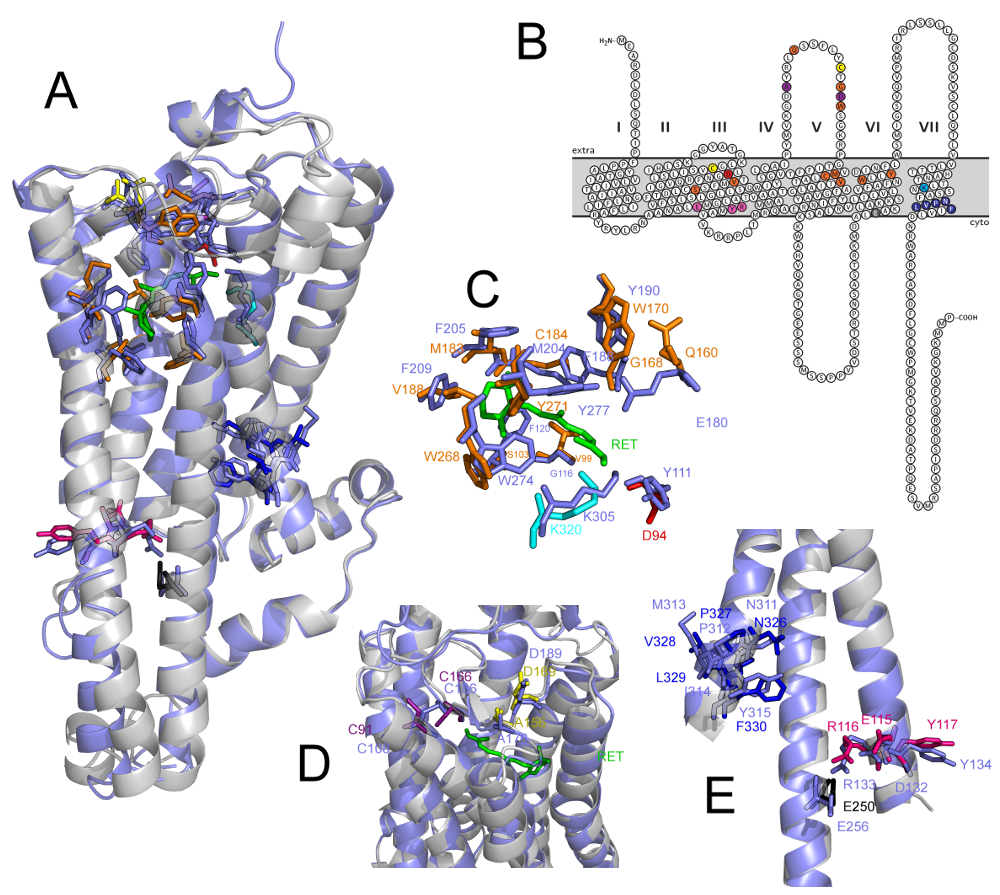
\includegraphics[width=4in]{./Chapter_RhodStruct/img/SpStructure.png}
  \caption[Structural details of the \textit{S. punctatus} chytriopsin homology model.]{Key \textit{S. punctatus} residues are colored according to function: orange (binding pocket residues), red (putative counterion), purple (disulfide bond), yellow (salt bridge), dark blue (NPxxY motif), and pink \& black (ion lock). Light purple functional and backbone residues belong to \textit{T. pacificus}, while grey backbone residues belong to \textit{S. punctatus}. The ideal position of the 11-\textit{cis}-retinal ligand, taken from the \textit{T. pacificus} crystal structure, is shown in green. A) C$\alpha$ backbone structural alignment of \textit{S. punctatus} homology model and \textit{T. pacificus} x-ray crystal structure, displayed in a cartoon representation, with key residues displayed as sticks. B) Topography plot of membrane spanning regions of \textit{S. punctatus} homology model. C) Detail of \textit{S. punctatus} binding pocket residues aligned with those of \textit{T. pacificus}. The lysine residue from \textit{S. punctatus} (cyan) is present in an optimal position to interact with the 11-\textit{cis}-retinal ligand (green), an aspect unique among the chytriopsins studied. The putative \textit{S. punctatus} counterion D94 (red) is also situated in an ideal position for photoisomerization. D) Detail of \textit{S. punctatus} disulfide bond (purple) and salt bridge (yellow) regions aligned with those of \textit{T. pacificus}. The view is from the top (extracellular side) of the protein, into the 11-\textit{cis}-retinal (green) binding pocket. E) Detail of \textit{S. punctatus} ERY and NPxxY regions aligned with those of \textit{T. pacificus}. In \textit{T. pacificus}, residues R133 and E256 (light purple) form a salt bridge in the inactive state to hold the structure in place, which is broken upon receptor activation. The corresponding \textit{S. punctatus} residues R116 (pink) and E250 (black) are in equivalent positions and presumably carry out the same function.}
  \label{fig:ChRhodS_SpStructure}
\end{figure}

%Non-covalent docking screen: Bden
\begin{figure}[hb]
  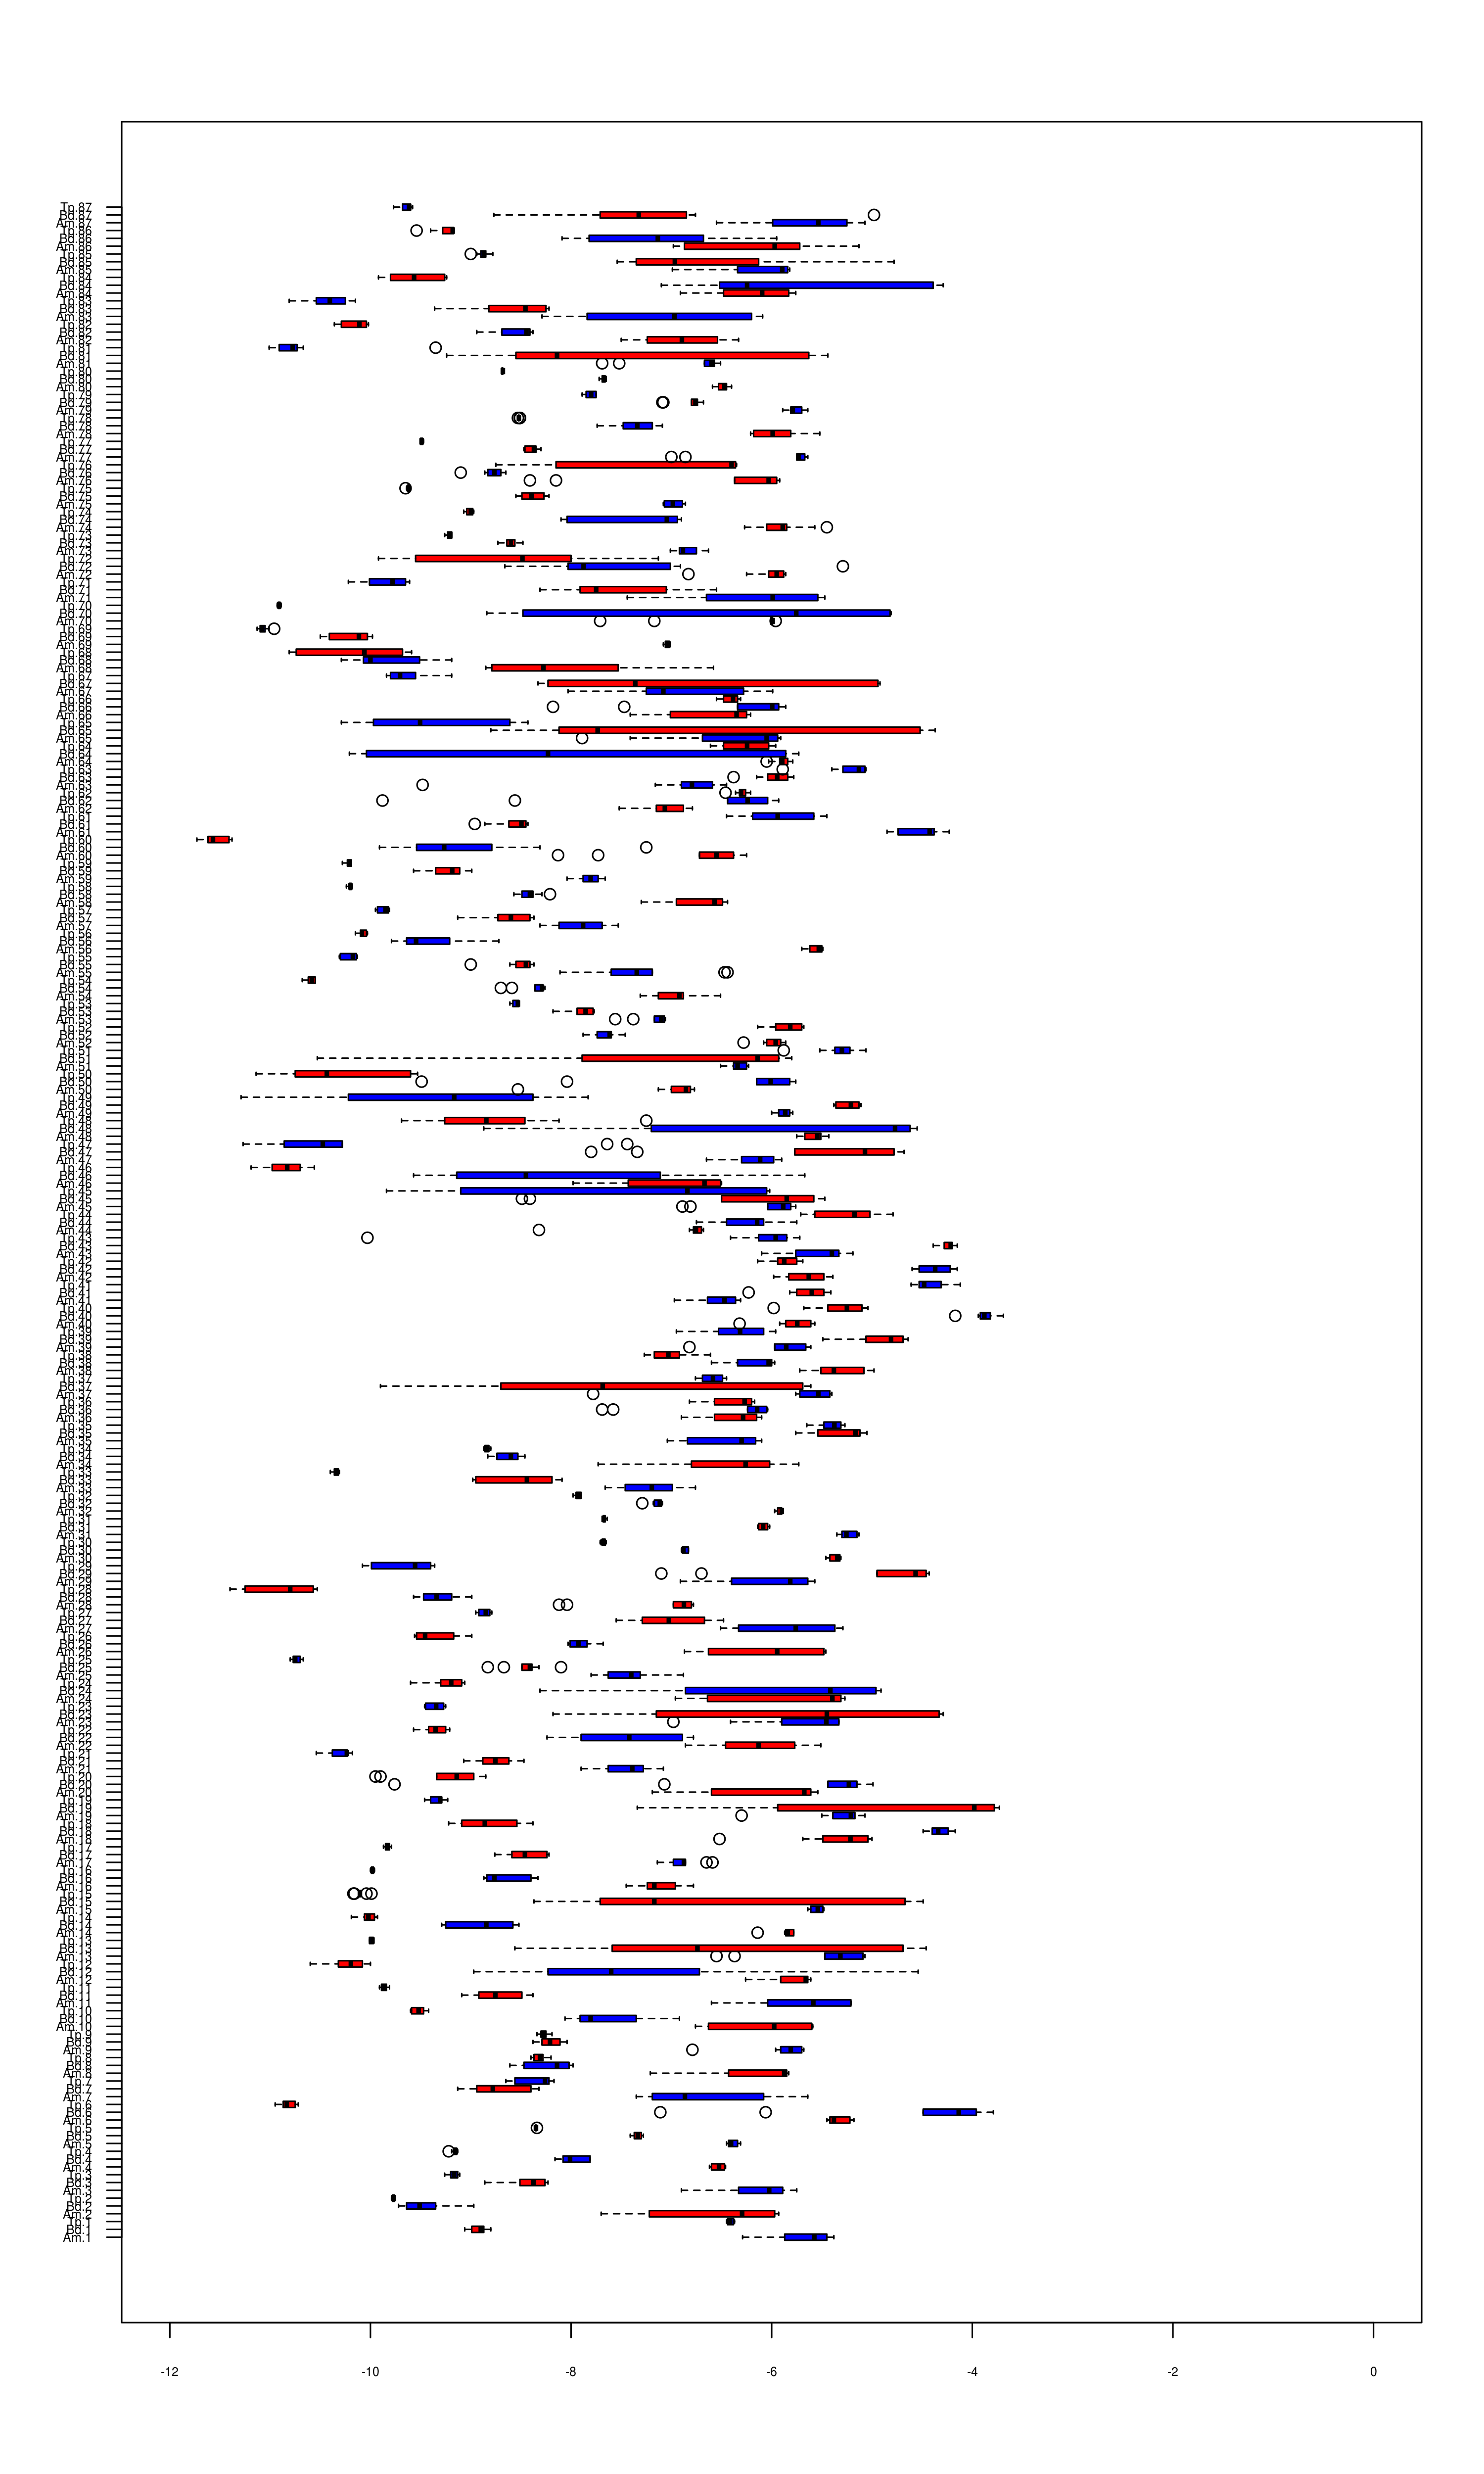
\includegraphics[]{./Chapter_RhodStruct/img/dockPlot.png}
  \caption[Docking screen for \textit{Bd} and \textit{Am} models]{A non-covalent docking screen using Autodock 4 and ligands obtained from ZINC against homology models for \textit{B. dendrobatidis} (red), \textit{A. macrogynus} (gray), and \textit{T. pacificus} (squid; 2Z73) (green). Histograms show distribution of ten lowest binding energies for protein-ligand conformations. Binding energy given on X-axis; ligand given on Y-axis. Ligands were obtained from ZINC database based on similarity to 11-\textit{cis}-retinal.}
  \label{fig:ChRhodS_NonCovDock}
\end{figure}

% MD analysis: Energy
\begin{figure}[hb]
  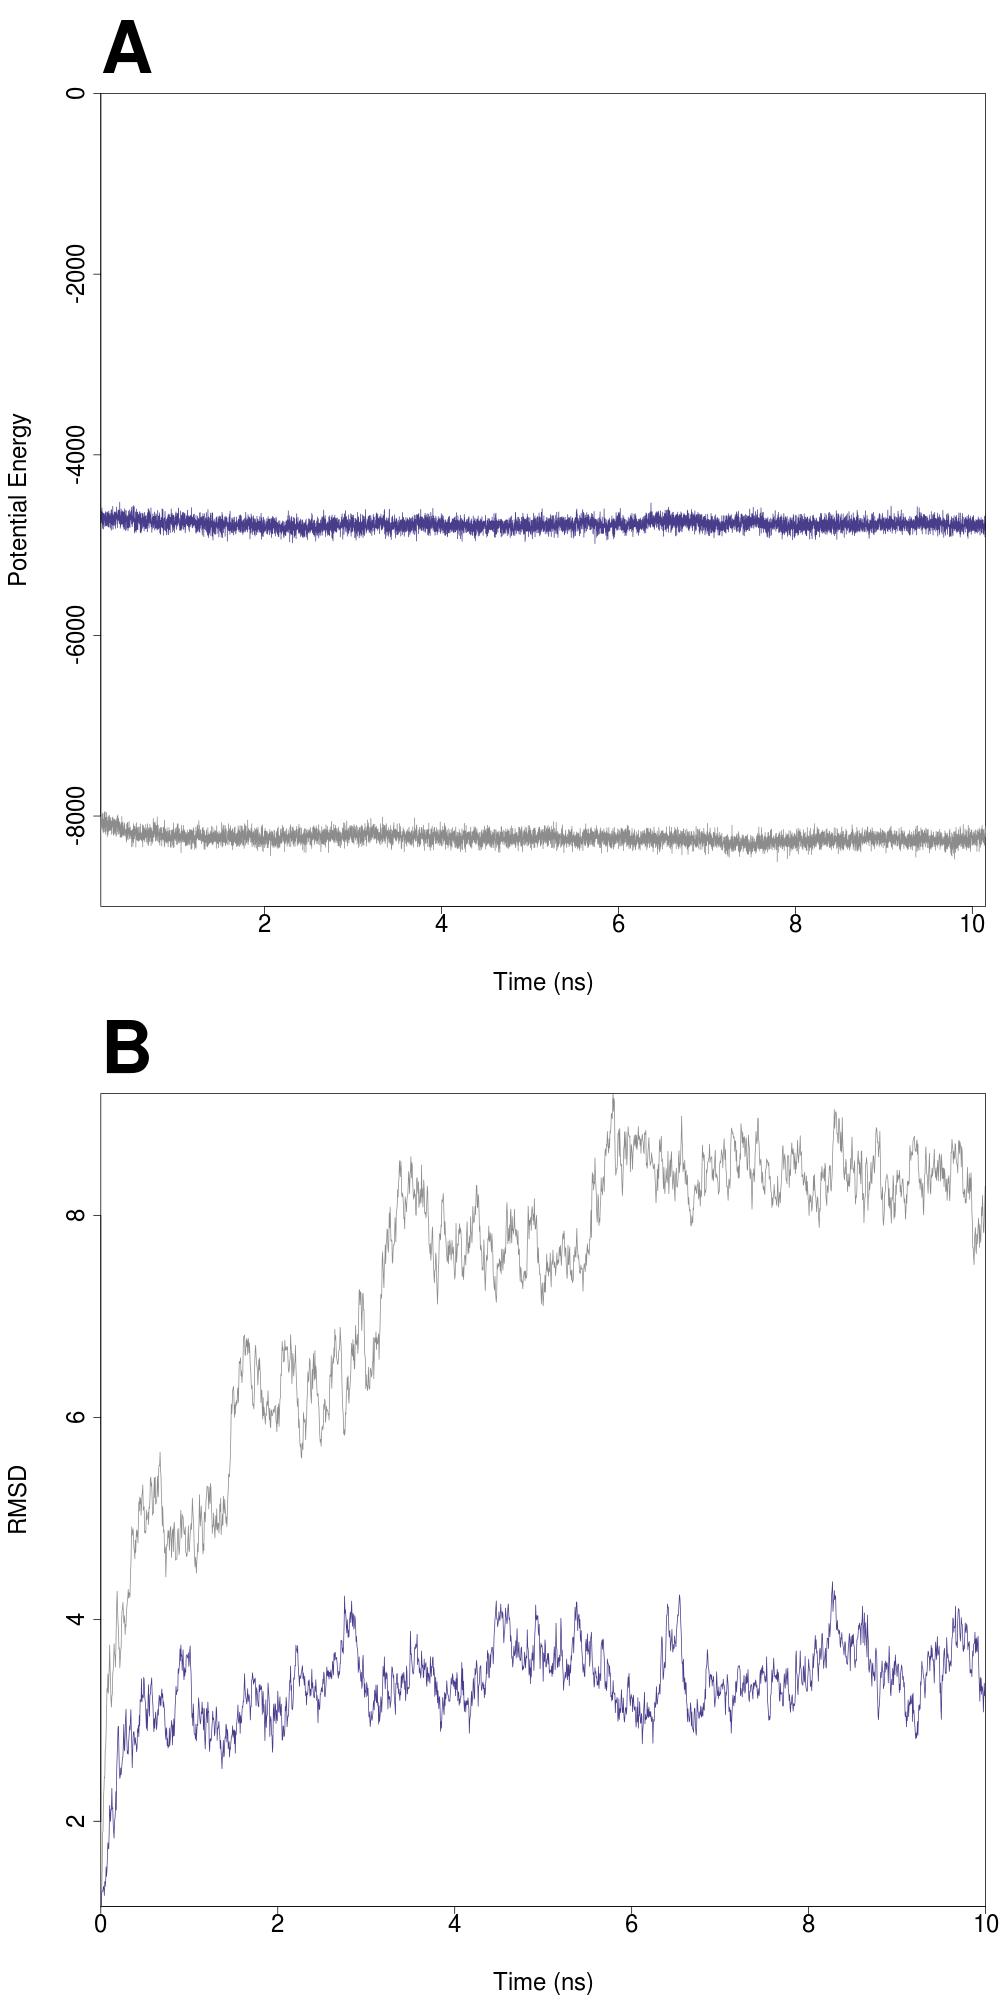
\includegraphics[width=4in]{./Chapter_RhodStruct/img/TpSp_mdoutRMS.png}
  \caption[MD summary plots]{Overview plots of MD simulation runs of squid 2Z73 crystal structure with 11-\textit{cis}-retinal (purple) and \textit{S. punctatus} model with 9-\textit{cis}-retinal (gray). A) Potential energy over course of simulation. During the simulation, both structures remain relatively stable. The \textit{S. punctatus} stucture has substantially lower potential energy than the squid structure. B) RMSd fits over course of simulation. The RMSd fit of the \textit{S. punctatus} structural model increases much more rapidly than that of the squid structure, but ultimately reaches a plateau after approximately 6 ns.}
  \label{fig:ChRhodS_MDEnergyRMSD}
\end{figure}

%%%%%%%%%%%%%%%%%%%%%%%%%%%%%%%%%%%%%%%%%%%%%%%%%%%%%%%%%%%%%%%%%%%%%%%
%% Document: Thesis for PhD at UC Riverside                          %%
%% Description: A comparative analysis of environment sensing in EDF %%
%% Author: Steven Ahrendt                                            %%
%%%%%%%%%%%%%%%%%%%%%%%%%%%%%%%%%%%%%%%%%%%%%%%%%%%%%%%%%%%%%%%%%%%%%%%
% RHODOPSIN TABLES %
%%%%%%%%%%%%%%%%%%%%

% PROCHECK results for homology models
% latex table generated in R 3.1.1 by xtable 1.7-3 package
% Mon Apr 20 16:19:46 2015
\begin{table}[tbp]
\centering
\begin{tabular}{rllllll}
  \hline
\hline
 & Spun & Bden & Amac & Tpac & Btau & Hsap \\ 
  \hline
Most favored regions & 90.7\% & 86.1\% & 66.4\% & 90.0\% & 79.2\% & 91.1\% \\ 
  Additional allowed regions & 7.5\% & 11.6\% & 24.1\% & 9.1\% & 15.8\% & 7.6\% \\ 
  Generously allowed regions & 1.2\% & 1.4\% & 6.0\% & 0.0\% & 3.8\% & 0.6\% \\ 
  Disallowed regions & 0.6\% & 0.9\% & 3.4\% & 0.0\% & 1.2\% & 0.6\% \\ 
   \hline
Verify3D & 73.60 & 55.41 & 131.62 & 87.85 & 109.14 & 00.0 \\ 
   \hline
\hline
\end{tabular}
\caption{PROCHECK Ramachandran plot results for chytriopsin and melatonin homology models, and animal rhodopsin crystal structures.} 
\label{tab:ChRhod_Procheck}
\end{table}
% RMSD of crystal structures
% latex table generated in R 3.1.1 by xtable 1.7-3 package
% Mon Apr 20 16:19:46 2015
\begin{table}[tbp]
\centering
\begin{tabular}{rrrrrrr}
  \hline
\hline
 & Spun & Bden & Amac & Tpac & Btau & Hsap \\ 
  \hline
Spun & 0.00 & 2.54 & 3.05 & 2.52 & 3.12 & 4.92 \\ 
  Bden & 2.54 & 0.00 & 3.33 & 2.55 & 2.70 & 5.11 \\ 
  Amac & 3.05 & 3.33 & 0.00 & 3.71 & 2.91 & 5.81 \\ 
  Tpac & 2.52 & 2.55 & 3.71 & 0.00 & 3.09 & 4.96 \\ 
  Btau & 3.12 & 2.70 & 2.91 & 3.09 & 0.00 & 5.50 \\ 
  Hsap & 4.92 & 5.11 & 5.81 & 4.96 & 5.50 & 0.00 \\ 
   \hline
\hline
\end{tabular}
\caption{Pairwise backbone RMSD measurements for chytriopsin and melatonin homology models, and animal rhodopsin crystal structures, calculated using the Bio3D package.} 
\label{tab:ChRhod_RMSD}
\end{table}
% Important Residues
% latex table generated in R 3.1.1 by xtable 1.7-3 package
% Mon Apr 20 16:19:46 2015
\begin{table}[tbp]
\centering
\begin{tabular}{rlllllll}
  \hline
\hline
 & Description & Bt1U19 & Tp2Z73 & Bd & Sp & Am & Cl15402 \\ 
  \hline
1 & Salt Bridge & R177 & A176 & K145 & A156 & T203 & -- \\ 
  2 & Salt Bridge & D190 & D189 & D158 & D169 & A223 & -- \\ 
   \hline
3 & Binding pocket & T118 & G116 & Q88 & V99 & Q139 & -- \\ 
  4 & -- & E122 & F120 & A92 & S103 & V143 & -- \\ 
  5 & Binding pocket & W265 & W274 & W317 & W268 & W468 & -- \\ 
  6 & H-bond core/Photoisomerase counterion & E181 & E180 & R149 & Q160 & -- & -- \\ 
  7 & -- & I189 & F188 & Y157 & G168 & -- & -- \\ 
  8 & Binding pocket/H-bond network w/Y268 & Y191 & Y190 & Y159 & W170 & -- & -- \\ 
  9 & -- & M207 & M204 & L173 & M183 & L237 & -- \\ 
  10 & -- & F208 & F205 & I174 & C184 & A238 & -- \\ 
  11 & -- & F212 & F209 & V178 & V188 & L242 & -- \\ 
  12 & Binding pocket & W265 & W274 & W317 & W268 & W468 & -- \\ 
  13 & Binding pocket/H-bond network w/Y191 & Y268 & Y277 & T320 & Y271 & Y471 & -- \\ 
   \hline
14 & Conserved Lysine & K296 & K305 & A347 & K320 & S498 & L336 \\ 
  15 & Counterion & E113 & Y111 & V83 & D94 & N134 & -- \\ 
   \hline
16 & [L]AxAD & L79 & L76 & V48 & L60 & L97 & -- \\ 
  17 & L[A]xAD & A80 & A77 & V49 & S61 & -- & -- \\ 
  18 & LAx[A]D & A82 & S79 & S51 & T63 & -- & -- \\ 
  19 & LAxA[D] & D83 & D80 & D52 & D64 & D101 & -- \\ 
   \hline
20 & DisulfideBond & C110 & C108 & C80 & C91 & C131 & -- \\ 
  21 & DisulfideBond & C187 & C186 & C155 & C166 & C220 & -- \\ 
   \hline
22 & [E]RY & E134 & D132 & N104 & E115 & E155 & -- \\ 
  23 & E[R]Y/IonicLock w/E247 & R135 & R133 & H105 & R116 & R156 & -- \\ 
  24 & ER[Y] & Y136 & Y134 & Y106 & Y117 & Y157 & -- \\ 
   \hline
25 & [N]PxxY & N302 & N311 & N353 & N326 & N504 & -- \\ 
  26 & N[P]xxY & P303 & P312 & P354 & P327 & P505 & -- \\ 
  27 & NP[x]xY & V304 & M313 & I355 & V328 & L506 & -- \\ 
  28 & NPx[x]Y & I305 & I314 & V356 & L329 & L507 & -- \\ 
  29 & NPxx[Y] & Y306 & Y315 & F357 & F330 & S508 & -- \\ 
   \hline
30 & IonicLock w/E247 & V138 & V136 & V108 & A119 & R159 & -- \\ 
  31 & IonicLock w/R135 & E247 & E256 & L299 & E250 & A450 & -- \\ 
   \hline
\hline
\end{tabular}
\caption{Conserved Rhodopsin motifs in X-ray crystal structures and chytropsin homology models. Abbreviations: Bt1U19=\textit{Bos taurus} X-ray crystal structure (PDBID 1U19); Tp2Z73=\textit{Todares pacificus} X-ray crystal structure (PDBID 2Z73);} 
\label{tab:ChRhod_motifs}
\end{table}


%%%%%%%%%%%%%%%%%%%%%%%%%%%%%%%
% RHODOPSIN AUXILLARY CHAPTER %
%%%%%%%%%%%%%%%%%%%%%%%%%%%%%%%
%%%%%%%%%%%%%%%%%%%%%%%%%%%%%%%%%%%%%%%%%%%%%%%%%%%%%%%%%%%%%%%%%%%%%%%%%%%%%%%%%
%% Document: Thesis for PhD at UC Riverside                                    %%
%% Title: Investigating the evolution of environmental and biotic interactions %%
%%          in basal fungal lineages through comparative genomics              %%
%% Author: Steven Ahrendt                                                      %%
%%%%%%%%%%%%%%%%%%%%%%%%%%%%%%%%%%%%%%%%%%%%%%%%%%%%%%%%%%%%%%%%%%%%%%%%%%%%%%%%%
% RHODOPSIN AUXILLARY CHAPTER %
%%%%%%%%%%%%%%%%%%%%%%%%%%%%%%%
\chapter{Rhodopsin related signaling pathways in basal fungi}
\label{chap:RhodAux}
\section{Introduction}
\indent G-protein coupled receptors (GPCRs) are a broad class of seven-transmembrane 
proteins which receive extracellular signals and initiate an intracellular response 
\cite{Lagerstrom2008}. This process is accomplished via signal transduction pathways 
which link certain effector proteins with the receptors using heterotrimeric GTP-binding 
and hydrolysing proteins (G proteins) \cite{Hepler1992}. There are two major pathways 
which GPCRs are principally associated with: the cAMP signaling pathway and the phosphatidylinositol pathway \cite{Gilman1987}.\\
\indent G protein complexes associate with a transmembrane GPCR and are loosely coupled to 
the intracellular side of the plasma membrane \cite{Clapham1997}.
These GTPases are composed of an $\alpha$, a $\beta$, and a $\gamma$ subunit. While the G$\alpha$ subunit 
was historically thought to be solely responsible for signal transduction \cite{Gilman1987}, 
it has been demonstrated that the G$\beta$/$\gamma$ subunit is capable of producing a 
response in yeast \cite{Clark1993}. Currently the number of effectors regulated by one 
or both subunits ($\alpha$ or $\beta$/$\gamma$) is equivalent \cite{Clapham1997}.\\ 
\indent The G$\alpha$ subunit is bound to a molecule of GDP in its inactive state. 
Upon receptor stimulation, for example photoisomerization of 11-\textit{cis}-retinal 
in rhodopsin, the bound GDP is exchanged for GTP and the now active G$\alpha$ subunit 
dissociates from both the receptor and the G$\beta$/$\gamma$ subunit \cite{Neves2002}.\\ 
\indent G$\alpha$ proteins of different types interact with difference downstream effectors. Four 
major G$\alpha$ protein subfamilies have been identified: G$_{s}$, G$_{i}$, G$_{q}$, and G$_{12}$ 
\cite{Hepler1992}. Additional fungal \cite{Bolker1998} and plant \cite{Ma1994} subfamilies exist 
as well. The type of G-protein to which the receptor is coupled can help classify the Type 2 
rhodopsins. The G$_{s}$ group contains the G$_{s}$ and G$_{olf}$  subunits, the latter being found 
in the olfactory neuroepithelial cells. These enzymes enhance the rate of cAMP synthesis by 
stimulating adenylate cyclase. Additionally, the G$_{s}\alpha$ subunit regulates Na$^{+}$ and 
Ca$^{2+}$ channels \cite{Hepler1992}. The G$_{i}$ group contains four subclasses: G$_{i}$, 
G$_{o}$, G$_{t}$, G$_{z}$. All G$_{i}$ subclasses possess a consensus sequence for 
ADP-ribosylation by pertussis toxin and function to inhibit adenylylcyclase \cite{KABMycotaIII}. 
G$_{o}$ proteins are abundant in the brain and implicated in membrane trafficking. 
G$_{t}$, or transducin, is activated by rhodopsin, activates cGMP-phosphodiesterase (cGMP-PDE) 
and closes cGMP-gated sodium channels. G$_{z}$ activity is relatively unknown, 
but evidence suggests that it inhibits adenylylcyclase activity as well \cite{KABMycotaIII}. 
The G$_{q}$ group contains members G$_{q}$, G$_{11}$, G$_{14}$, G$_{15}$, and G$_{16}$. 
These are widely expressed and involved in signal transduction through activation of phospholipase C-$\beta$1 \cite{KABMycotaIII}. 
Finally, the G$_{12}$ group contains the G$_{12}$ and G$_{13}$ subunits.\\
\indent Motifs that describe the fungal group come from seven identified fungal G$\alpha$ proteins with no similarity to G$\alpha$ proteins of the previously identified groups. In \textit{S. cerevisiae}, the GP1 protein functions as a mating factor, while the GP2 protein functions in intracellular cAMP regulation. Members of the plant group may play a role in signal transduction from hormone receptors.\\
\indent GTP-bound G$\alpha$ proteins are themselves acted on by a regulator of G protein signaling (RGS) protein \cite{DeVries2000}. RGS proteins are responsible for the rapid return of active GTP-bound G$\alpha$-subunits to their inactive state, and function to tightly regulate the signal generated by a GPCR. \\
\indent Activated G$\alpha$ proteins also interact with the $\gamma$-subunit of cGMP phosphodiesterase. Phosphodiesterases (PDEs) are a class of enzymes which cleave phosphodiester bonds. One specific group is the cyclic nucleotide phosphodiesterases, which act on cAMP and cGMP. Due to this activity, they are importance regulators of signal transduction. In mammalian systems, for example, they associate with activeated G$\alpha$ subunits in order to close cGMP-gated cation channels located in the plasma membrane and regulate the influx of Ca$^{2+}$ and Na$^{+}$. One such interaction is the associateion between transducin (G$_{t}$) and cGMP phosphodiesterase in the rhodopsin visual signaling cascasde [citation needed].\\
\indent Six $\beta$-subunits and twelve $\gamma$-subunits have been identified \cite{}. The observed diversity is lower than
 69 expected as not all possible $\beta$-$\gamma$ pairs are cabple of forming.\\
\indent The G$\beta$/$\gamma$ subunit is responsible for a number of regulatory functions during 
 74 signal transduction \cite{Clapham1997}.
\indent Structurally, the G$\beta$ subunit contains a 20aa $\alpha$-helix
 77 region and a large domain composed of repeated WD40 motifs. While the WD-repeat region is unknown, it is presumed
 78 to be related to assembly of the complex. \cite{Clapham1997}.\\
\indent Additionally, at least four $\beta$-subunits and six $\gamma$-subunits have been identified \cite{Hepler1992} in Fungi.
\indent All G$\gamma$ subunits posess specific CaaX motifs at their C-termini. These motifs are subject to 
postranslational modification, the nature of which both targets the G$\beta$/$\gamma$ complex to 
the plasma membrane, and governs interactions between G$\gamma$ and G$\alpha$, receptors, and/or 
effector proteins \cite{Krystofova2005}.\\
\indent There are two major pathways which GPCRs are principally associated with: the cAMP signaling pathway and the phosphatidylinositol pathway \cite{Gilman1987}.\\
\indent As discussed in Chapter~\ref{chap:RhodStruct}, rhodopsins are a broad class of photosensitive 
seven-transmembrane proteins which respond to light through photoisomerization of a retinaldehyde chromophore, 
typically 11-\textit{cis}-retinal. Type 2 rhodopsins are GPCRs which function in, among other things, metazoan visual pathways.\\
\indent The work in this chapter deals with presence and absence of components of the 
rhodopsin signaling pathway in basal fungi, including the distribution of heterotrimeric 
G protein subunits and potential effector proteins.\\

%%-- Chapter methods --%%
\section{Methods}
\subsection*{Identification of homologous photosensory proteins}
To get a sense for the distribution of photosensory proteins in fungi, the fungal proteomes listed in Table~\ref{tab:AppData_Taxon} were searched using the classes of photosensory proteins from previous analyses described in by Idnurm et al. The white collar protein complex, comprising WC-1 and 2, were searched for using the \textit{N. crassa} proteins NCU02356 and NCU00902, respectively, as queries using $ssearch36$ with an e-val cutoff of 1e-10. Type 1 and Type 2 opsins were searched for using HMMER (v3.0) $hmmsearch$ with Pfam HMM models PF01036 and PF00001, respectively, using an e-val cutoff of 1e-20. Cryptochrome homologs were searched using HMMER (v3.0) $hmmsearch$ with an HMM generated from the 20 seed sequences in the PFAM domain PF12546 (Cryptochrome\_C). Hits were retained above a threshold of 1e-20. Similarly, phytochrome homologs were searched using $hmmsearch$ with an HMM profile generated from the 80 seed sequences in PF00360 (PHY). Hits were retained above a threshold of 1e-20.\\
\subsection*{G protein Analysis}
Homologs of G$\alpha$ proteins were identified using HMMER (v3.0) $hmmsearch$ with an HMM profile generated from the seed set of PFAM domain family PF00503. Fungal hits above a threshold of e-20 were kept for subsequent analysis. A maximum likelihood tree was constructed using RAxML (v7.5.4) with 100 bootstrap replicates using representative Fungal hits from basal fungi, Zygomycete, Ascomycete, and Basidiomycete lineages, along with representative outgroup eukaryotic G$\alpha$ sequences from the G$_{s}$ (IPR000367), G$_{q}$ (IPR000654), G$_{i}$ (IPR001408), and G$_{12}$ (IPR000469) families.\\
\indent Homologs of G$\beta$ proteins were identified using HMMER (v3.0) $hmmsearch$ with an HMM profile generated from the seed set of PRINTS domain family PR00319. Fungal hits above a threshold of e-100 were kept for subsequent analysis. A maximum likelihood tree was constructed using RAxML (v7.5.4) with 100 boostrap replicates using fungal hits from basal lineages, Zyogomycete, Ascomycete, and Basidiomycete lineages, along with representative sequences for Gnb-1, Gnb-2, Gnb-3, Gnb-4, and Gnb-5 from mouse and human. Also included were other outgroup sequences from Psoj, Crei, and Dmel.\\
\indent Homologs of G$\gamma$ proteins were identified using HMMER (v3.0) $hmmsearch$ with an HMM profile generated from 43 sequences matching the InterPro IPR001770 domain: 1 Choanoflagellate, 2 Porifera, 1 Placozoa, 1 Ctenophora, 6 Cnidaria, 1 Nematoda, 6 Arthropoda, and 25 Chordata. Fungal hits above a threshold of e-5 were kept for phylogenetic analysis, along with a representative set from the original IPR001770 dataset: 1 Choanoflagelatte, 12 Chordata, 1 Placozoa, and 2 Porifera. \\
\indent Homologs of RGS proteins were identified using HMMER (v3.0) $hmmsearch$ with an HMM profile genearated from the seed set of PFAM domain family PF00615.\\
\indent Multiple sequence alignments were drawn and annotated using the \TeXshade package \cite{Beitz2000texshade}, and protein domain figures were drawn using the pgfmolbio package (\url{http://www.ctan.org/pkg/pgfmolbio}).\\
\subsection*{Effector Analysis}
\indent Homologs of phospohodiesterase (PDE) subunits were identified using sequences from KEGG families K08718 ($\alpha$), K13756 ($\beta$), and K13759 ($\gamma$). Each KEGG family contained a set of phylogenetically diverse sequences from which HMM models were built using T-coffee (v) and HMMER (v3.0). K08718 (PDE$\alpha$) contained xxxx, K13756 (PDE$\beta$) contained yyyy, and K13759 (PDE$\gamma$) contained zzzz.\\
\indent Phospholipase C (PLC) proteins were searched using HMM from seed from PF00388.\\
\subsection*{Maintenance of chytrid cultures}
\textit{B. dendrobatidis} JEL423 cultures were grown on 1\% Tryptone plates [tryptone (10 g/L), glucose (3.2 g/L), and 1\% agar] and maintained at 23$^{\circ}$C. \textit{S. punctatus} SW-1 cultures were grown on PmTG agar plates [peptonized milk (0.5 g/L), tryptone (1 g/L), glucose (5 g/L), and 1\% agar]. All cultures were maintained at room temperature (23$^{\circ}$C) under an unregulated lighting scheme. Motile zoospores, were collected from actively growing (2-4 day old) plates by flooding with 2-4 mls of sterile di H$\_{2}$O, waiting 30-45 minutes, and collecting the liquid. \\
\subsection*{Phototaxis}
To examine the extent of phototaxis in \textit{B. dendrobatidis} and \textit{S. punctatus}, I followed the protocol outlined by Muehlstein et al.\nocite{Muehlstein1987} to observe phototaxis in the marine Chytridiomycete \textit{Rhizophydium littoreum}. Briefly, light was projected upwards through the bottom of a 60mm plastic petri dish containing a concentrated (approx. 10$^{6}$ cells/ml) suspension of freshly harvested, motile (approx. 75\%) zoospores. An "X" pattern is cut in a piece of dark cardboard which is placed between the light source and the petri dish. Phototaxis is determined by zoospore aggregation, avoidance, or ignorance of the "X"-shaped light source, and is scored as attraction, aversion, or absence, respectively. The light source was a Kodak slide projector with 300W white light bulb and was redirected using a stainless steel cosmetic mirror. The light source was placed at a distance such that a light intensity of 950 lux was achieved. Phototaxis experiments were carried out in a darkroom at 25$^{\circ}$C.\\ 
\subsection*{\textit{Pichia pastoris} heterologous expression}
Genomic DNA was extracted using a modified bead-beating procedure. Briefly, approximately 100 mg of material containing both zoospores and sporangia was scraped from actively-growing, zoospore-rich \textit{B. dendrobatidis} and \textit{S. punctatus} plates. The material was added to approximately 100 mg of silicon beads \emph{[size]} and mixed with 600 $\mu$l of Cell lysis solution \emph{[Qiagen, cite]} and 3 $\mu$l of proteinase K \emph{[cite]}. The solution was homegenized with a bead beater using a 30s pulse at 4$^{\circ}$C and subsequently incubated for 2h at 55$^{\circ}$C. 200 $\mu$l of protein precipitation solution \emph{[Qiagen, cite]} was added to the mixture and iced for 15 min. After centrifugation at 14000xg for 3 min at room temperature, the supernatant was collected, mixed with 600 $\mu$l isopropanol, and spun at 1400xg for 1 min at room temperature. Pellet was washed with 600 $\mu$l ice cold 70\% EtOH and spun at 1400xg for 1 min at room temperature. Finally the pellet was air dried for 15 min at room temperature, resuspended in 50 $\mu$l H$_{2}$O, incubated at 65$^{\circ}$C for 1 hr, and stored at -20$^{\circ}$C.\\
\indent For plasmid construction, the \textit{B. dendrobatidis} rhodopsin gene was cloned into the pHIL-S1 \textit{P. pastoris} expression plasmid using a strategy described previously \cite{Bieszke1999}.  Modifications to the \textit{B. dendrobatidis} gene include the addition of 5' and 3' EcoRI restriction sites, as well as a C-terminal hexahistidine epitope. These modifications were accomplished using the following PCR primers (provided in Appendix B): "Bden\_EcoRI\_F" (forward) and "Bden\_EcoRI\_His\_R" (reverse). PCR conditions were as follows: 10 $\mu$l 5X buffer, 27.5 $\mu$l H2O, 5 $\mu$l of each primer (10 $\mu$M), 1 $\mu$l of 10 mM dNTPs, 1 ng DNA, and 0.5 $\mu$l Phusion Polymerase in each 50 $\mu$l reaction. Cycle parameters used were 98$^{\circ}$C for 30s, 30 rounds of: 95$^{\circ}$C for 5s, 58$^{\circ}$C for 20s, 72$^{\circ}$C for 30s, and a final 72$^{\circ}$C for 10 min. The resulting fragment was purified using the Qiagen PCR purification kit, digested with EcoRI, purified again, and inserted into the EcoRI site of the pHIL-S1 plasmid. The resulting BdpHIL-S1 plasmids were transformed into chemically competent \textit{E. coli} JM109 cells. Transformants were checked for proper insertion / orientation by colony PCR.\\ 
\indent The \textit{S. punctatus} gene was synthesized and inserted into the pHIL-S1 vector by GenScript (GenScript USA Inc. Piscataway, NJ 08854). Two versions were constructed: a wild type, which codes for the conserved lysine residue, and a mutant, which replaces the lysine residue with alanine.  \\
\indent The NoppHIL-S1 vector containing the Nop-1 protein previously described in \textit{Neurospora crassa} \cite{Bieszke1999} was generously loaned from Dr. Katherine Borkovich at the University of California, Riverside. The availability of sequences used for these analyses is provided in the appendix.\\
\indent For expression and membrane preparation, the BdpHIL-S1, SppHIL-S1, NoppHIL-S1, and pHIL-S1 vectors were cloned into \textit{P. pastoris} strain GS115 using the strategy described previously by Bieszke et al. \nocite{Bieszke1999} for expresion of Nop-1. The transformation vectors were linearized overnight with StuI. A 500 ml culture of \textit{P. pastoris} was grown in Medium A [yeast extract (10 g/L), proteose peptone (20 g/L), and dextrose (20 g/L)] shaking at 250rpm and at 30$^{\circ}$C until A$_{600}$ = 2.1. The culture was split into two 250 ml samples and spun at 1500g for 5 minutes at 4$^{\circ}$C. The pellets were resuspended in 250 ml ice-cold H$_{2}$O, spun again, resuspended in 100 ml ice-cold H$_{2}$O, spun again, and resuspended in 1 ml ice-cold 1M sorbitol. The cells were transferred to 1.5 ml microfuge tube on ice and used in transformation by electroporation. 80 $\mu$l of cells were added to 10 $\mu$l of linearized vector, iced for 5 minutes, and electroporated using 2 mm gap cuvettes and the following parameters: voltage gradient: 7.5 kV/cm, resistance: 600 $\Omega$, capacitance: 25 $\mu$F. Transformants were screened for integration of the plasmids by PCR. One of each transformant was grown on a large scale as described previously \cite{Bieszke1999}.\\
\indent Harvested cell pellets were washed in 1 pellet volume of ice-cold, sterile water and centrifuged at 1500xg for 5 min at 4$^{\circ}$C. The pellets were subsequently washed and resuspended in 1 pellet volume of Buffer A (7 mM NaH2PO4, pH 6.5, 7 mM EDTA, 7 mM dithiothreitol, 1 mM PMSF). Acid-washed 0.5mm glass beads were used to disrupt 1 ml aliquots using three 1-min pulses and two 90-s pulses with a minibead beater at 4$^{\circ}$C. The supernatants were collected and pooled to yield the cell lysate. The lysate was layered on a 70\% sucrose cushion (w/v in Buffer A) and centrifuged with no braking at 92000xg for 1 hour at 4$^{\circ}$C in a SW27 swinging bucket rotor. The membrane layer, located at the interface between the lysate and sucrose cushion, was collected, stored at 4 $^{\circ}$C, and used for the membrane preparation.\\
\indent Immunoblot analysis on the membrane preparation was conducted using 50 $\mu$g of protein by PAGE. Mouse anti-6X His monoclonal antibody (Fisher Scientific) was used at both 1:1000 and 1:3000 dilution for the primary antibody. Goat anti-mouse (Bio-Rad) was used as the secondary antibody at a 1:5000 dilution.\\

%%-- Chapter results --%%
\section{Results}
\subsection*{Photosensory}
In order to expand on previous summaries (eg \cite{Idnurm2010}) of the extent of photosensing in fungi, I searched for known photosensory proteins within proteomes (Table~\ref{tab:AppData_taxa}) of sequenced fungi from across the kingdom, with a focus on the recently sequenced basal lineages. This search included White-Collar complex proteins, Phytochromes, Cryptochromes, and opsins (Type 1 and 2). The results (Figure~\ref{fig:ChRhodA_photosenseSurvey}) are consistent with previous reviews but provided a higher level of resolution in the basal lineages, particularly the Chytridiomycota and Blastocladiomycota.\\
\indent It is worth noting here that the basal fungal genomes surveyed have different capacities for photosensing. In \textit{Spizellomyces punctatus}, both a Type 2 rhodopsin and White collar complex members are identified, the structure of the former of which is elaborated upon in Chapter~\ref{chap:RhodStruct}. This rhodopsin protein is the only known so far in chytrids which posesses the critical lysine residue important for proper rhodopsin function \cite{Smith2010}. In \textit{Batrachochytrium dendrobatidis} however, the only photosensory protein identified is the Type 2 rhodopsin, which does not appear to posess the critical lysine residue. Yet the proteome of its closest relative, the non-pathogenic \textit{Homolaphlyctis polyrhiza}, contains an apparent opsin-GC fusion protein, the likes of which have only recently been described in the Blastocladiomycete \textit{Blastocladiella emersonii} \cite{Avelar2014}. This architecture is also observed in the three other Blastocladiomycete organisms, \textit{Allomyces macrogynus}, \textit{Catenaria anguillalae}, and the transcriptome of \textit{Coelomomyces lativittatus} (described in more detail in Chapter~\ref{chap:ClatTranscriptome}). Structural features of these opsin-GC fusion proteins are explored further in Chapter~\ref{chap:RhodStruct}.\\
\subsection*{G protein Analysis}
Multiple G$\alpha$ proteins were identified at an e-val < 1e$^{-20}$ in all surveyed chytrid genomes. Counts of predicted proteins are presented in Figure~\ref{fig:ChRhodA_photosenseSurvey}.\\
\indent One of the \textit{S. punctatus} G$\alpha$ proteins, SPPG05404, contains a C-terminal pertussis toxin sensitivity motif (C[GAVLIP]{2}X) and is 76.8\% identical to \textit{N.crassa} GNA-1 (NCU06493). Similarly, \textit{A. macrogynus} contains two predicted G$\alpha$ proteins, AMAG03583 and AMAG04903, both of which have the same motif. These proteins are approximately 70\% identical to \textit{N. crassa} GNA-1 (71.2\% and 69.6\%, respectively). Additionally, all of these proteins contain an N-terminal myristoylation motif (MGXXXS), consistent with members of the G$_{i}$ subfamily. \textit{R. allomycis}, possesses one protein with a pertussis toxin motif and has 69.77\% identity to \textit{N. crassa} GNA-1. \textit{Piromyces sp.} possesses two proteins (18092 and 48456) with pertussis motifs. Only the former, however, also posesses an N-terminal myristoylation motif. It is 73.7\% identical to \textit{N. crassa} GNA-1. The latter appears have a large portion of its N-terminus truncated relative to the former, and is more similar to \textit{N. crassa} GNA-3 than GNA-1 (65.7\% vs 55.2\% identity).\\
\indent Two proteins from \textit{B. dendrobatidis}, BDEG06989 and BDEG06990, have high similarity to GNA-1 at 66.3\% and 73.7\% identity, respectively. However, only BDEG06989 contains an N-terminal myristoylation motif. Neither of them contain the C-terminal pertussis motif.\\
\indent SPPG05884 from \textit{S. punctatus} has 75.6\% identity to \textit{N. crassa} GNA-1, but lacks the C-terminal pertussis motif (however it contains the N-terminal myristoylation motif).\\
\indent \textit{G. prolifera} posesses two predicted proteins with high (approx. 74\%) similarity to \textit{N. crassa} GNA-1. Both contain N-terminal myristoylation motifs, however only one also contains the C-terminal pertussis motif. A third predicted protein contains the myristoylation motif and is 62.6\% identical to \textit{N. crassa} GNA-3.\\
\indent The similarities of all identified chytrid G$\alpha$ proteins to identified \textit{N. crassa} G$\alpha$ proteins are described in Table~\ref{tab:ChRhodAux_Gcomp}.\\
\indent A multiple sequence alignment, highlighting the pertussis and myristoylation motifs shared among all fungal G$\alpha$ proteins containing such motifs is presented in Figure~\ref{fig:ChRhodA_gaMSA}.\\
\indent A phylogenetic analysis was performed on all identified fungal G$\alpha$ proteins using RaxML (Figure~\ref{fig:ChRhodA_GalphaTree}). The majority of identified but uncharacterized chytrid G$\alpha$ proteins were most closely related to the Group IV family. This group remains largely uncharacterized, though there is evidence to suggest that the \textit{Ustilago maydis} homolog is induced during pathogenic development \cite{Bolker1998}. All other characterized G$\alpha$ groups (I, II, and III) contain chytrid members, suggesting an ancient origin for these families. The fungal and mammalian G$\alpha$ proteins represent distinct groups.\\
\indent All surveyed chytrids were predicted to possess one or more G$\beta$ proteins. Counts and percent identity with \textit{N. crassa} GNB-1 are presented in Tables~\ref{fig:ChRhodA_photosenseSurvey} and Table~\ref{tab:ChRhodA_Gcomp}. A phylogenetic
tree is given in Figure~\ref{fig:ChRhodA_GbetaTree} which shows sequences from basal lineages
clustering among each other. All identified fungal sequences possess multiple WD40 repeat domains
typical of G$\beta$ proteins identified with InterproScan (Figure~\ref{img:ChRhodA_GbetaStruct}). \\
\indent \textit{A. macrogynus}, \textit{B. dendrobatidis}, \textit{H. polyrhiza}, \textit{Orpinomyces}, and \textit{Piromyces} were each predicted to possess a single G$\gamma$ protein (e-val < 1e-5). Of these identified G$\gamma$ proteins, only those from \textit{B. dendrobatidis} \textit{Orpinomyces} contained a classic pertussis toxin sensitivity motif of the form (C[GAVLIP]\{2\}X), with 51.4\% and xx.x\% identity to NCU00041 (\textit{N. crassa} GNG-1). Counts and percent identity with \textit{N. crassa} GNG-1 are presented in Figure~\ref{fig:ChRhodA_photosenseSurvey} and Table~\ref{tab:ChRhodA_Gcomp}. Multiple sequence alignment of fungal sequences recovered which posess the pertussis motif is provided in Figure~\ref{fig:ChRhodA_ggMSA}.\\
\indent In chytrids, RGS homologs were predicted in \textit{R. allomycis}, \textit{S. punctatus}, and \textit{B. dendrobatidis}. The two \textit{Sp} proteins shared 22.1\% and 18.8\% identity with the \textit{N. crassa} RGS protein NCU08319 \cite{Borkovich2004}, while the \textit{Bd} and \textit{R. allomycis} proteins shared 17\% and 13.4\% identity, respectively, with NCU08319. One of the \textit{Sp} proteins (SPPG07577) contained a G$\gamma$ binding region motif (GGL domain: PF00631), while SPPG04061 did not. The \textit{Bd} protein (BDEG00728) contained the GGL domain as well.\\
\subsection*{Effector Proteins}
A search of effector proteins associated with G protein signaling pathways encompassed the phosphodiesterase, phospholipase, 
and RGS protein families (Figure~\ref{fig:ChRhodA_photosenseSurvey}). PDE $\alpha$ and $\beta$ subunit homologs were recovered 
in the basal lineages. In most cases, the recovered protein had significant similarity to both $\alpha$ and $\beta$ queries. 
Maximum likelihood phylogenetic analysis (Figure~\ref{fig:ChRhodA_PDEtree}) places recovered fungal proteins as distinct from metazoan lineages, with the exception of one sequence belonging in \textit{H. polyrhiza}.\\ 
\subsection*{Phototaxis and Heterologous Protein expression}
In order to determine the phototactic abilities of \textit{B. dendrobatidis} and \textit{S. punctatus}, I followed the procedure outlined in \cite{Muehlstein1987} for \textit{Rhizophydium littoreum}. However, no phototaxis was observed in either \textit{B. dendrobatidis} or \textit{S. punctatus}. Furthermore, zoospores of \textit{H. polyrhiza} were not collected at sufficiently high quantities for meaningful phototaxis observation.\\
\indent Heterologous protein expression of the chytrid opsin proteins was not observed using either BdpHIL-S1 or SppHIL-S1 vectors, despite successful expression using NoppHIL-S1 (Figure~\ref{fig:ChRhodA_PichiaBlot}).\\ 

%%-- Chapter conclusions --%%
\section{Discussion}
The goals for the research in this chapter were to assess, in the basal fungi, the complement of proteins which are secondarily involved in the rhodopsin-mediated photosignaling cascade (ie proteins other than the rhodopsin GCPR protein, including the intermediate heterotrimeric G proteins, and the effectors involved in the cAMP signaling and phosphotidylinositol pathways. From a functional perspective, this comparative study will demonstrate which of the basal fungi have a complete pathway, and would be helpful in understanding at which point in evolution these components were lost.\\
\indent G$\alpha$ subunits posessing N-terminal myristoylation and C-terminal pertussis motifs are members of the G$_{i}$ subfaimly. Transducin is one member of this family, and is known to associate with rhodopsin to function to activate cGMP-PDE. \textit{S. punctatus} and \textit{A. macrogynus} posess G$\alpha$ proteins which contain these motifs and which have high similarity to \textit{N. crassa} Gna-1. In \textit{N. crassa}, \emph{$\Delta$gna-1} strains are deficient in multiple pathways during both vegetative and sexual development, one of which (macroconidiation and mass accumulation) seems to be related to photosensing \cite{Ivey1996}.\\
\indent The G$\alpha$ group in fungi can be classified into four families \cite{Bolker1998}. Chytrid G$\alpha$ proteins are present in all four of these families. Multiple G$\alpha$ proteins in \textit{Bd} and \textit{Hp} appear to fall within the fungal Group IV (for which there is no \textit{N. crassa} homolog, however there is an \textit{Ustillago maydis} homolog implicated in pathogenicity).\\
\indent Phototaxis was not observed in the motile zoospores of \textit{B. dendrobatidis} or \textit{S. punctatus} when [SA: rephrase]following experimental protocol laid out [SA: //]for \textit{Rhizophydium littoreum} \cite{Muehlstein1987}, despite the presence of presumably active photoreceptor proteins in these organisms. There is no prior evidence of phototaxis in these species, only observed in \textit{Allomyces reticulatus} \cite{Saranak1997} and \textit{R. littoreum} \cite{Muehlstein1987}. One hypothesis as to the lack of phototaxis is that perhaps the GPCR type 2 rhodopsins are not used in phototaxis, but govern another light-regulated response mechanism. While the receptors are present, the downstream associated effectors and response-related protein components are not. This interpretation is supported by the fact that \textit{Bd} and \textit{Sp} do not posess PDE-$\gamma$ subunit homologs, which are known to have functions related to hyperpolarization and which could thus be related to flagellar beating.\\
\indent The lack of heterologous protein expression using the \textit{Pichia pastoris} cloning system was unexpected given the successes enjoyed with expression of the Bovine rhodopsin \cite{Abdulaev1997} and an opsin protein identified in \textit{N. crassa} \cite{Bieszke1999}. This lack of expression for chytropsins from \textit{B. dendrobatidis} and \textit{S. punctatus} using the BdpHIL-S1 and SppHIL-S1 vectors, respectively, can potentially be attribituted to the long intracellular loop regions found in these proteins introducing sufficient disorder so as to impede proper folding and membrane integration. For comparision, the cytoplasmic loop 3 (CL3) regions in Bovine rhodopsin (1U19) and Nop1 are only 6 and 8 amino acids long, respectively, whereas the CL3 regions in \textit{Bd} and \textit{Sp} are 99 and 36 amino acids long, respectively.\\

%%%%%%%%%%%%%%%%%%%%%%%%%%%%%%%%%%%%%%%%%%%%%%%%%%%%%%%%%%%%%%%%%%%%%%%
%% Document: Thesis for PhD at UC Riverside                          %%
%% Description: A comparative analysis of environment sensing in EDF %%
%% Author: Steven Ahrendt                                            %%
%%%%%%%%%%%%%%%%%%%%%%%%%%%%%%%%%%%%%%%%%%%%%%%%%%%%%%%%%%%%%%%%%%%%%%%
% RHODOPSIN FIGURES %
%%%%%%%%%%%%%%%%%%%%%

% Presence/absence heatmap for photosensory proteins and accessory components
\begin{figure}[hb]
  \centering
  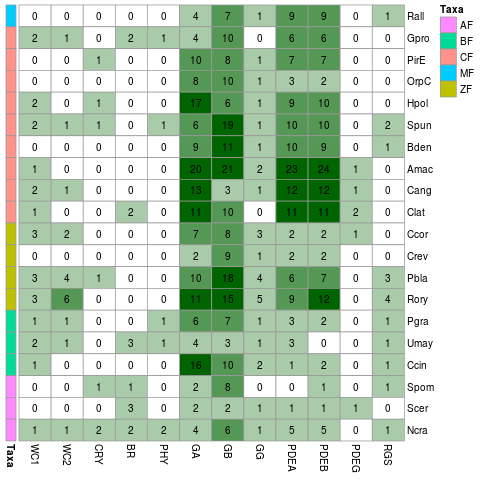
\includegraphics[width=4in]{./Chapter_RhodAux/img/photosenseHeatmap.png}
  \caption[Photosensory survey]{Photosensory protein distribution and G protein signalling pathway component distribution}
  \label{fig:ChRhodA_photosenseSurvey}
\end{figure}

% Galpha msa
\begin{figure}[hb]
  \centering
  \begin{texshade}{./Chapter_RhodAux/dat/FungalGA_PM.fasta_aln}
    \threshold[80]{50}
    \setdomain{1}{1..15,340..355}
    \showruler{1}{top}
    \feature{top}{1}{MGXXXS}{brace[Red]}{Myristoylation [Red]}
    \feature{top}{1}{351..355}{brace[Blue]}{Pertussis [Blue]}
    \hidenumbering
  \end{texshade}
  \caption[Galpha MSA]{Multiple sequence aligment of N-termini and C-termini. G$\alpha$ proteins identified in fungi which posessed both N-terminal myristoylation (MGXXXS) and C-terminal pertussis (C[GAVLIP]{2}X) motifs were aligned using T-coffee.}
  \label{fig:ChRhodA_gaMSA}
\end{figure}

% Galpha tree
\begin{figure}[hb]
  \centering
  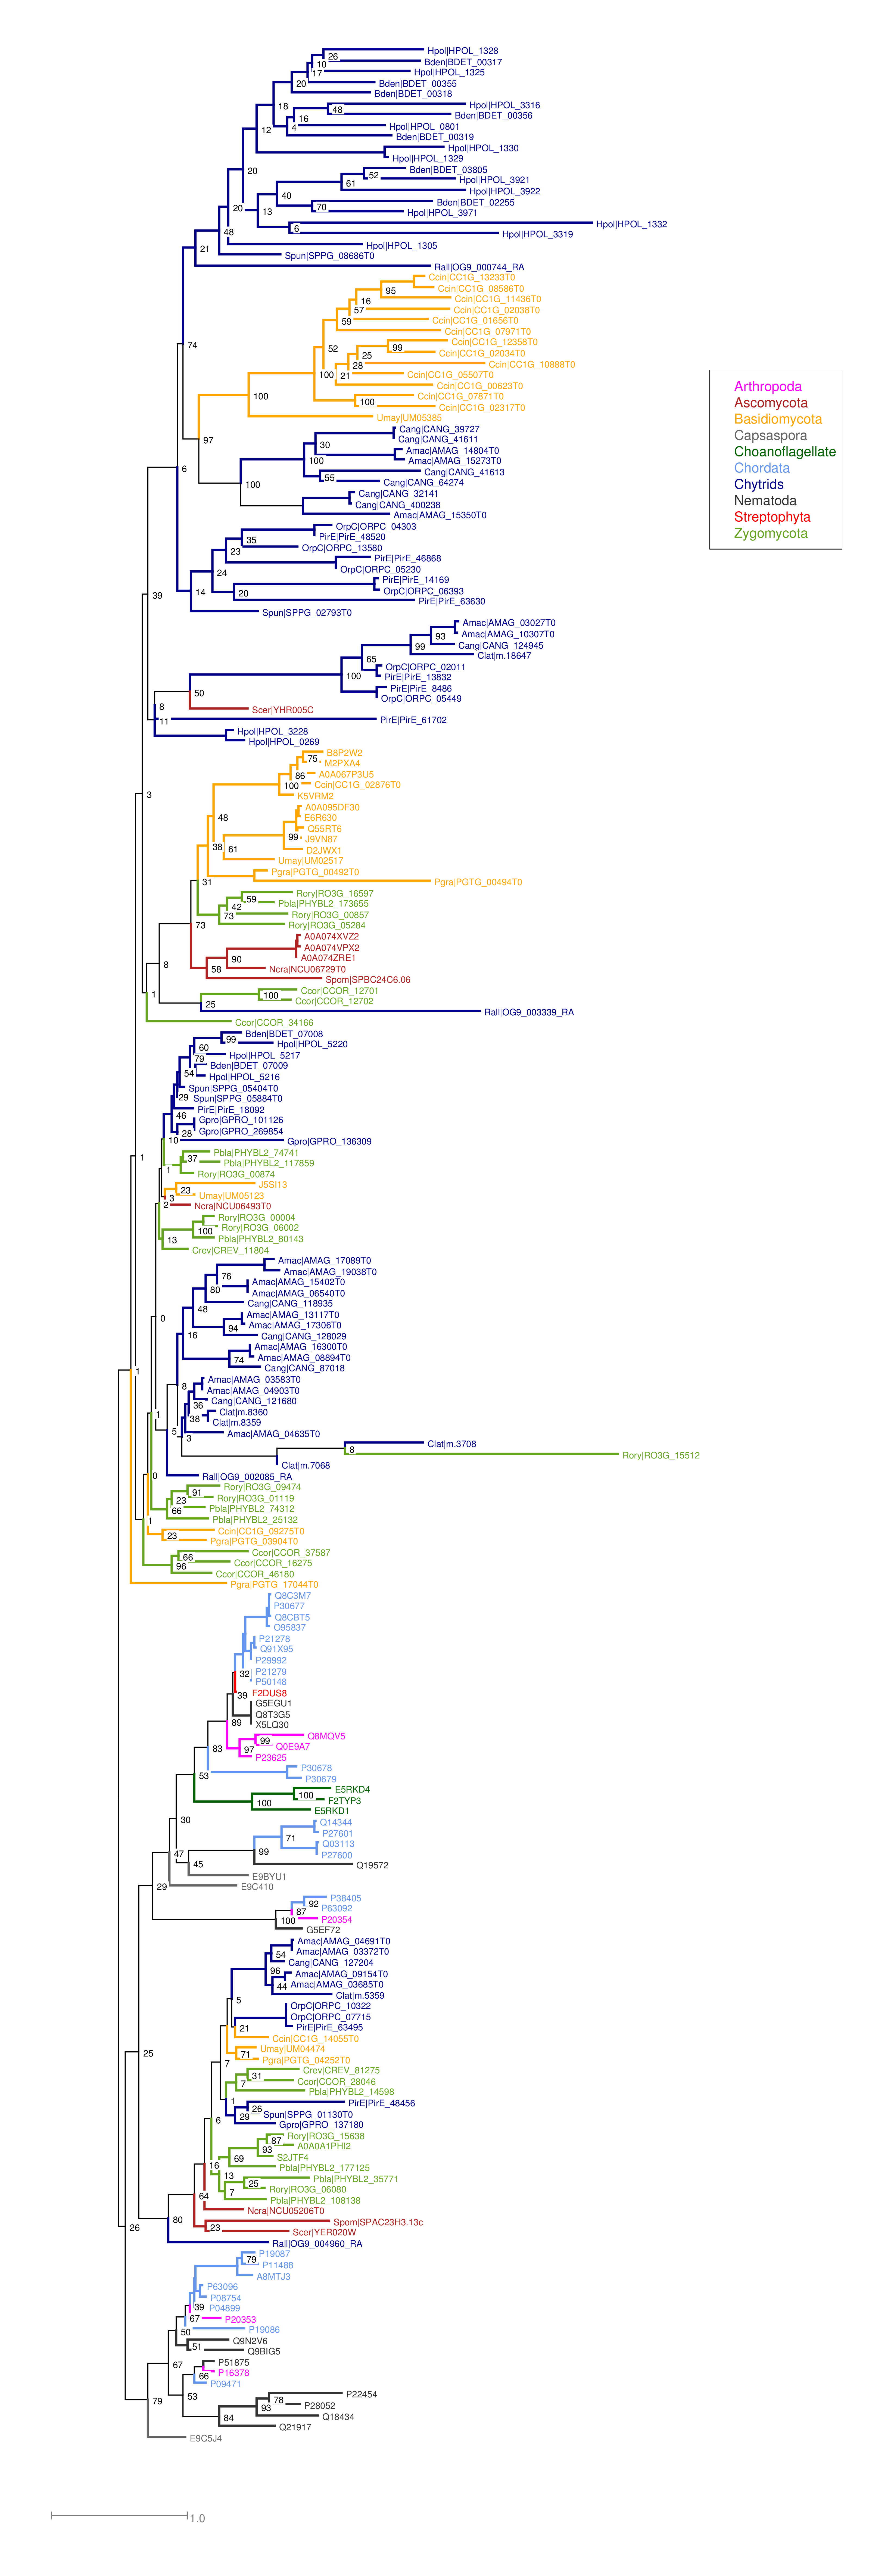
\includegraphics{./Chapter_RhodAux/img/Galpha_tree.png}
  \caption[G$\alpha$ tree]{Maximum likelihood tree of identified G-$\alpha$ subunits in fungi and animal outgroups}
  \label{fig:ChRhodA_GbetaTree}
\end{figure}

% Gbeta structure
\begin{figure}[hb]
  \centering
  \begin{texshade}{./Chapter_RhodAux/dat/FungalGB.fasta_aln}
    \shadingmode[allmatchspecial]{similar}
    \shadingcolors{grays}
    \fingerprint{500}
    \showlegend
    \feature{top}{NCU00440T0}{61..98,153..186,233..271,111..140,289..315,191..229,321..356}{,-,}{WD}
  \end{texshade}
  \caption[G$\beta$ WD40 repeats]{Schematic of identified fungal G$\beta$ proteins highlighting conservation and location of multiple WD40 repeat domains}
  \label{fig:ChRhodA_GbetaStruct}
\end{figure}

% Gbeta tree
\begin{figure}[hb]
  \centering
  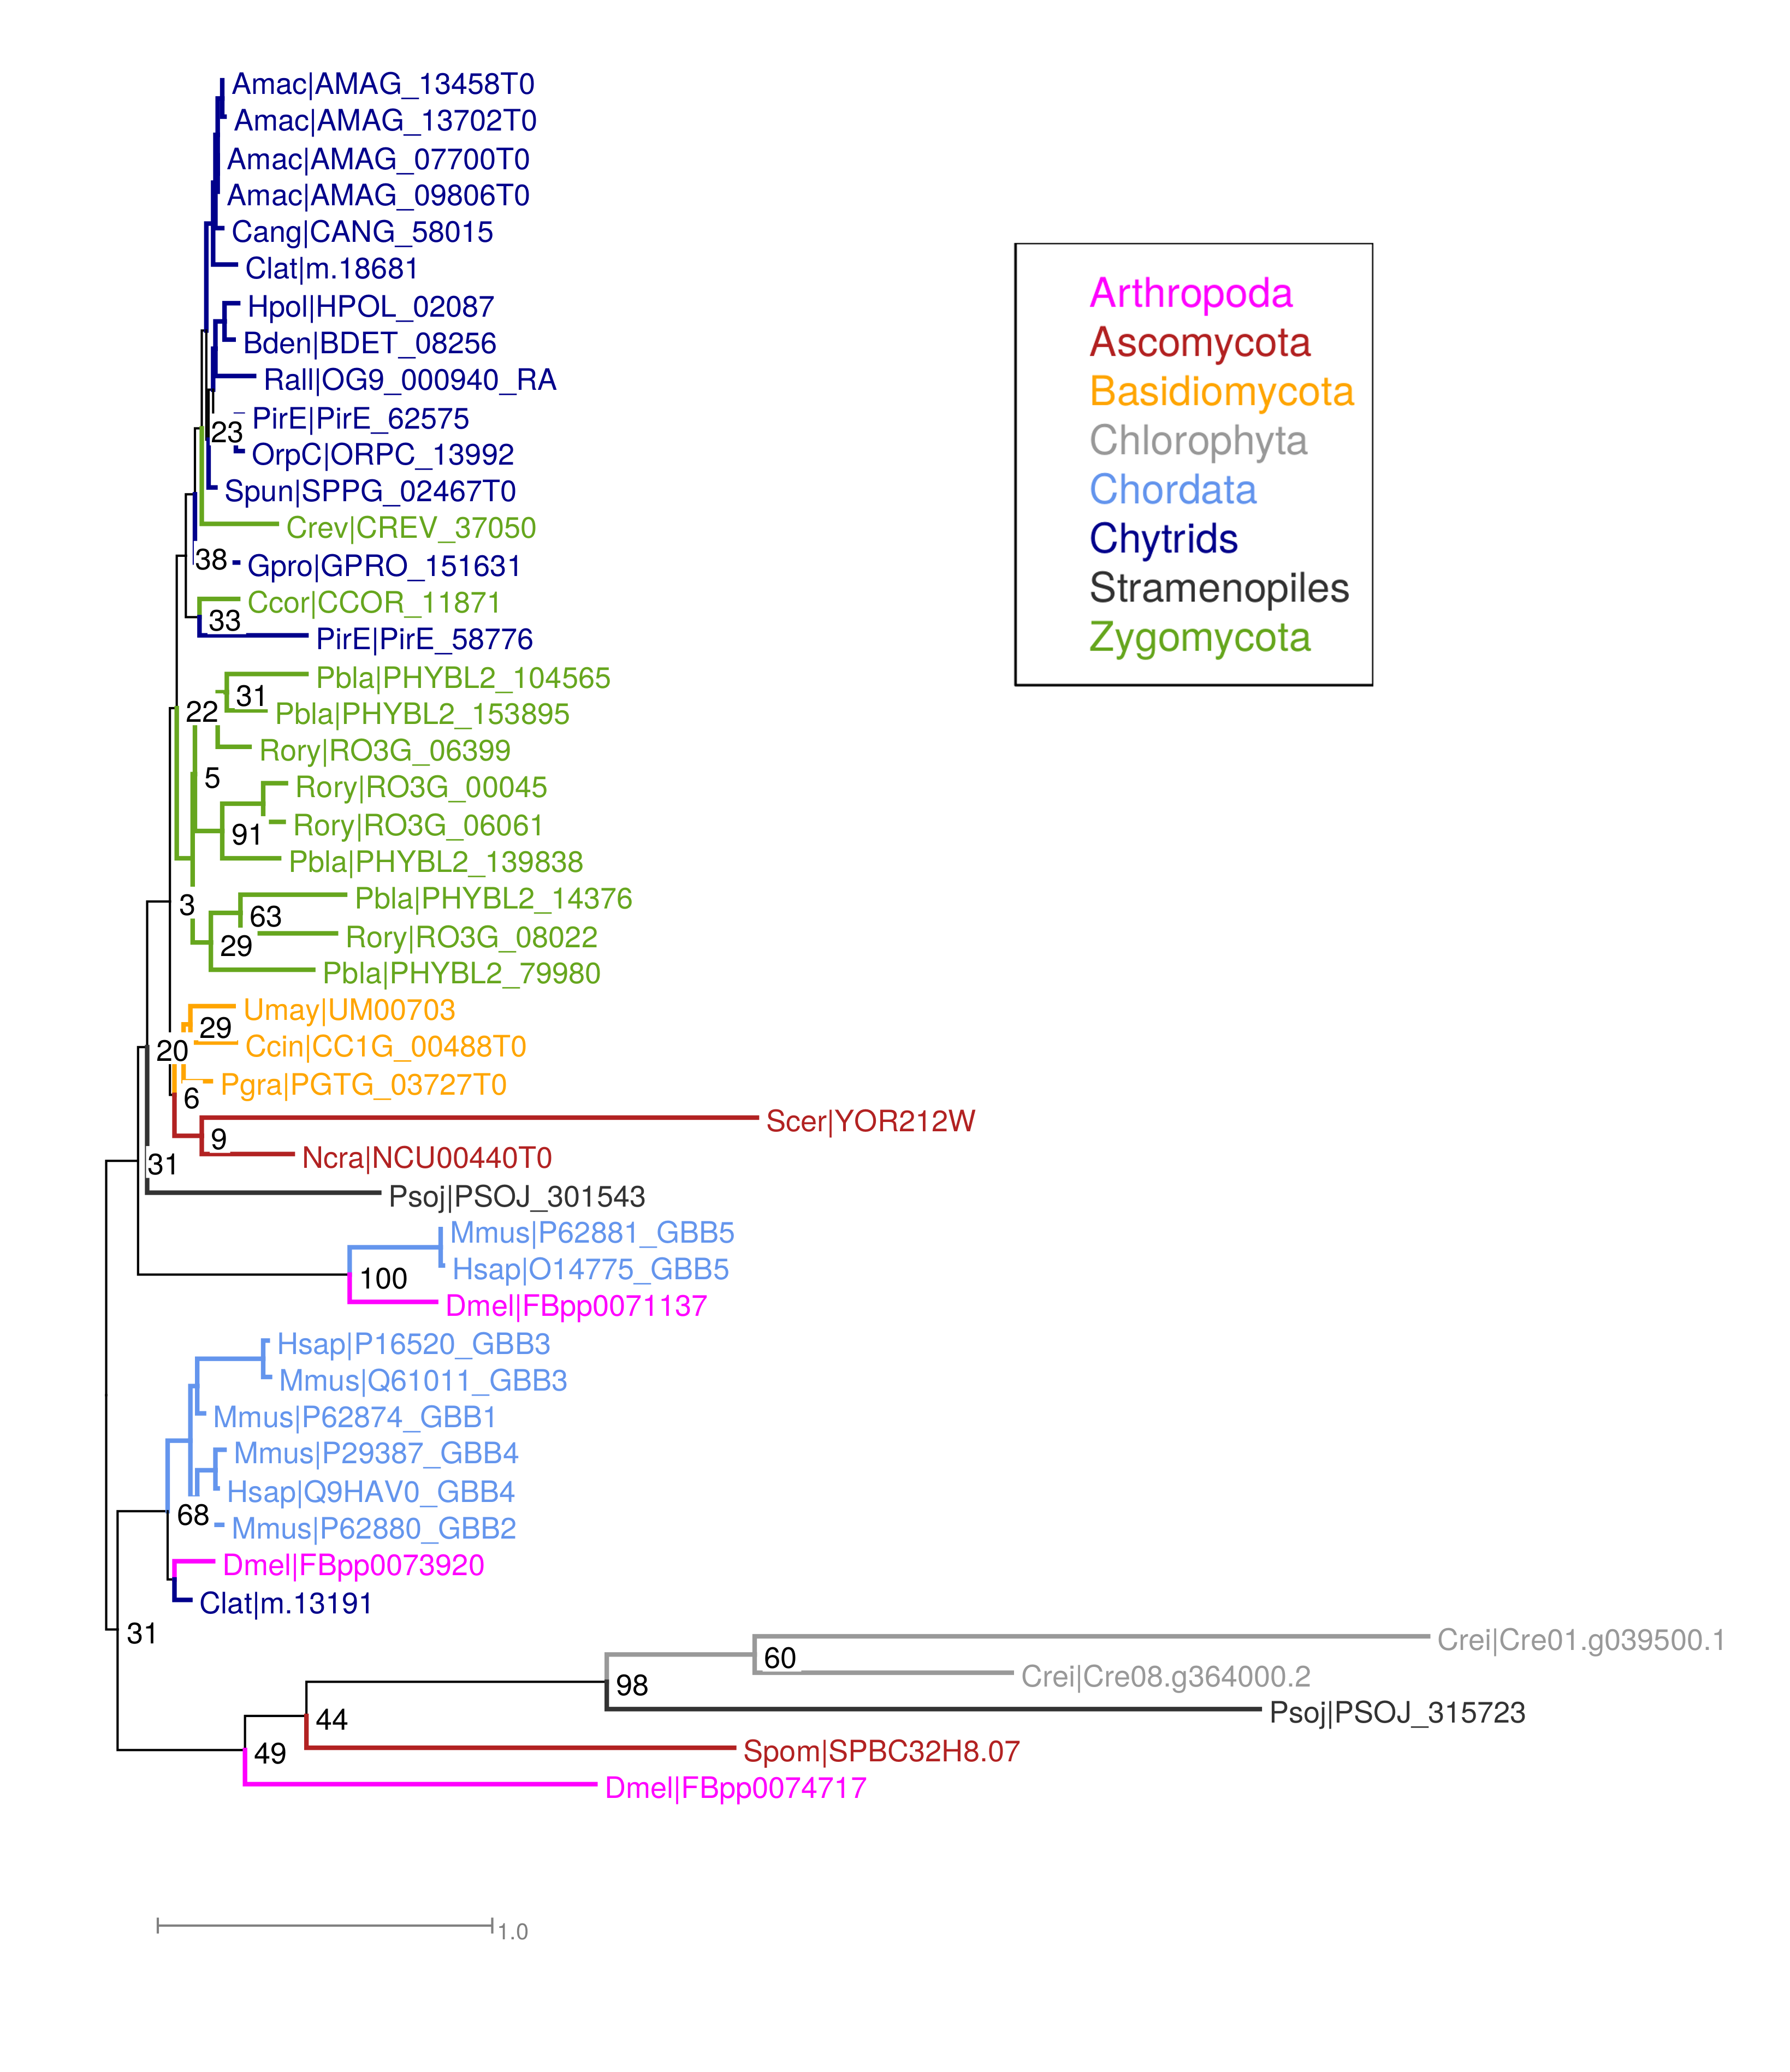
\includegraphics{./Chapter_RhodAux/img/Gbeta_tree.png}
  \caption[Gbeta tree]{Maximum likelihood tree of identified G-beta subunits in fungi and animal outgroups}
  \label{fig:ChRhodA_GbetaTree}
\end{figure}

% Ggamma msa
\begin{figure}[hb]
  \centering
  \begin{texshade}{./Chapter_RhodAux/dat/FungalGG.fasta_aln}
    \threshold[80]{50}
    \setends{1}{45..70}
    \showruler{1}{top}
    \feature{top}{1}{62..65}{brace[Blue]}{Pertussis [Blue]}
    \hidenumbering
  \end{texshade}
  \caption[Galpha MSA]{Multiple sequence aligment of G$\gamma$ proteins identified in fungi which posessed C-terminal pertussis (C[GAVLIP]{2}X) motifs aligned using T-coffee.}
  \label{fig:ChRhodA_ggMSA}
\end{figure}

% Ggamma tree
\begin{figure}[hb]
  \centering
  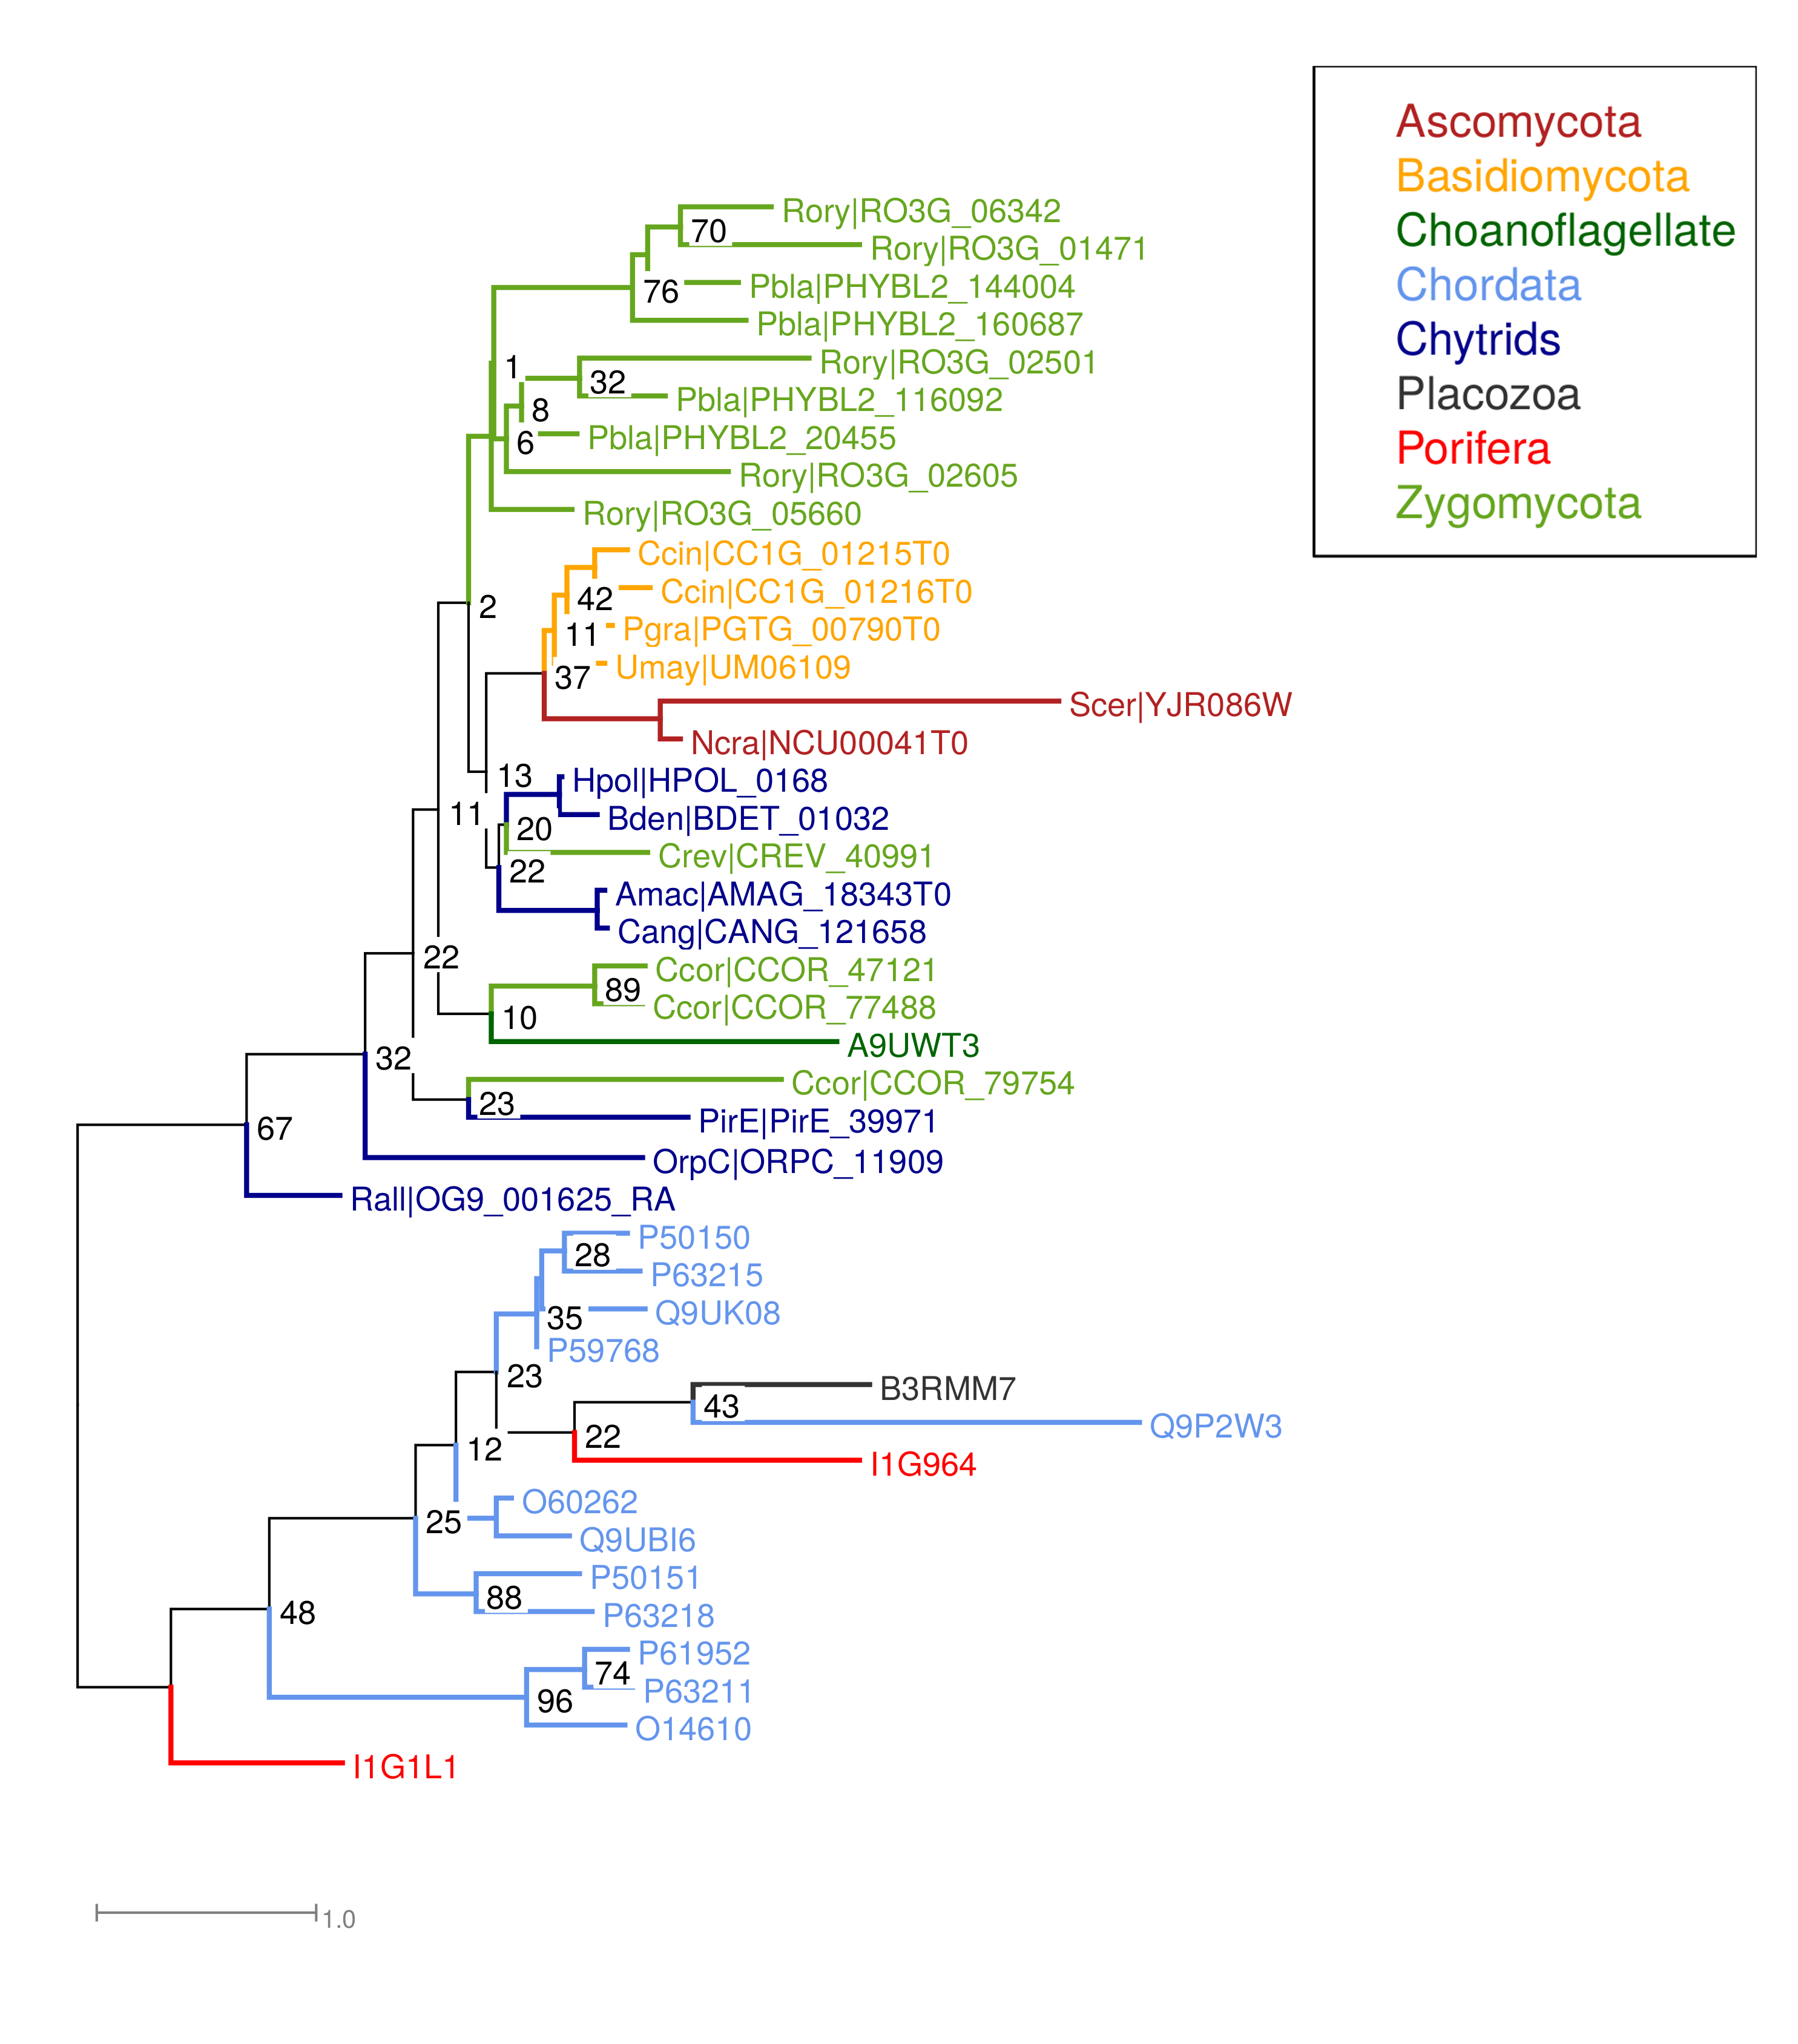
\includegraphics{./Chapter_RhodAux/img/Ggamma_tree.png}
  \caption[Gbeta tree]{Maximum likelihood tree of identified G$\gamma$ subunits in fungi and animal outgroups}
  \label{fig:ChRhodA_GgammaTree}
\end{figure}

% RGS structure
\begin{figure}[hb]
  \centering
  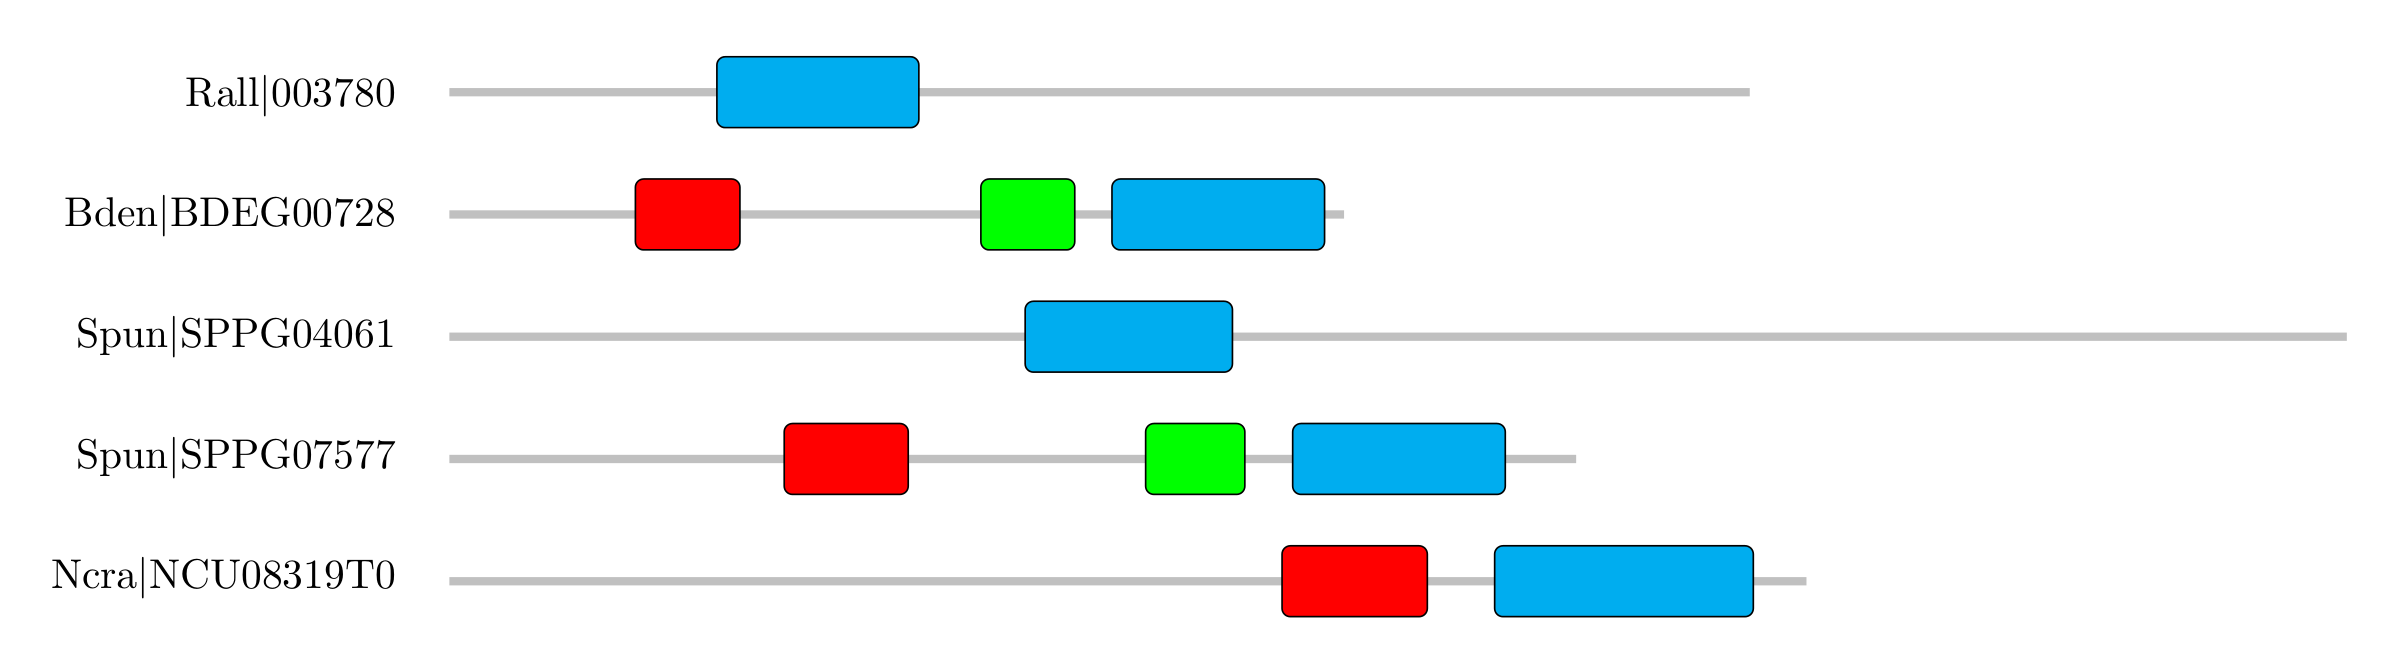
\includegraphics{./Chapter_RhodAux/img/ChyNcra_RGS.png}
  \caption[RGS proteins]{Structural domains of RGS proteins identified from HMM search in chytrids.}
  \label{fig:ChRhodA_RGS}
\end{figure}

%%%%%%%%%%%%%%%%%%%%%%%%%%%%%%%%%%%%%%%%%%%%%%%%%%%%%%%%%%%%%%%%%%%%%%%%%%%%%%%%%
%% Document: Thesis for PhD at UC Riverside                                    %%
%% Title: Investigating the evolution of environmental and biotic interactions %%
%%          in basal fungal lineages through comparative genomics              %%
%% Author: Steven Ahrendt                                                      %%
%%%%%%%%%%%%%%%%%%%%%%%%%%%%%%%%%%%%%%%%%%%%%%%%%%%%%%%%%%%%%%%%%%%%%%%%%%%%%%%%%
%% RHODOPSIN TABLES %%
%%%%%%%%%%%%%%%%%%%%%%

% G-protein subunit counts
%<<label=ChRhodAux_Gprot,echo=FALSE,results=tex>>=
%library(xtable)
%data <- read.table("../dat/Gabg_counts.tsv",sep="\t",header=T,check.names=FALSE,stringsAsFactors=FALSE)
%data$Species <- paste("\\emph{",data$Species,"}",sep="")
%colnames(data)[-1] = c("G$\\alpha$","G$\\beta$","G$\\gamma$")
%xdata <- xtable(data,label="tab:ChRhodAux_Gprot",caption=c("(long) G protein subunits identified through sequence similarity","(short) G protein distribution"))
%hlines <- c(-1,-1,0,3,6,nrow(xdata),nrow(xdata))
%print(xdata,
%      table.placement="tbp",
%      caption.placement="bottom",
%      hline.after=hlines,
%      include.rownames=FALSE,
%      sanitize.text.function=identity
%)
%@

% G protein comparisons
% latex table generated in R 3.0.1 by xtable 1.7-4 package
% Sat May 23 09:13:09 2015
\begin{table}[tbp]
\caption[G$\alpha$ subunit comparison]{first} 
\label{tab:ChRhodA_Gcomp}
\centering
\begin{tabular}{llllll}
  \hline
Species & Class & Name & Broad & NCBI & Identity$^{a}$ \\ 
  \hline
\emph{Neurospora crassa } & I & GNA-1 & NCU06493$^{pm}$ & - & 100 \\ 
  \emph{-} & II & GNA-2 & NCU06729 &  & 100 \\ 
  \emph{-} & III & GNA-3 & NCU05206$^{m}$ &  & 100 \\ 
  \emph{Allomyces macrogynus} & I & - & AMAG\_03583$^{pm}$ & - & 71 \\ 
  \emph{-} & I & - & AMAG\_04903$^{pm}$ & - & 69 \\ 
  \emph{-} & I & - & AMAG\_15273 & - & 88 \\ 
  \emph{-} & I & - & AMAG\_04635$^{m}$ & - & 68 \\ 
  \emph{-} & I & - & AMAG\_17306$^{m}$ & - & 65 \\ 
  \emph{-} & I & - & AMAG\_13117$^{m}$ & - & 65 \\ 
  \emph{-} & I & - & AMAG\_15402$^{m}$ & - & 61 \\ 
  \emph{-} & I & - & AMAG\_06540$^{m}$ & - & 61 \\ 
  \emph{-} & I & - & AMAG\_16300$^{m}$ & - & 57 \\ 
  \emph{-} & I & - & AMAG\_08894$^{m}$ & - & 57 \\ 
  \emph{-} & I & - & AMAG\_17089 & - & 57 \\ 
  \emph{-} & III & - & AMAG\_03685$^{m}$ & - & 64 \\ 
  \emph{-} & III & - & AMAG\_09154$^{m}$ & - & 64 \\ 
  \emph{-} & III & - & AMAG\_03372$^{m}$ & - & 62 \\ 
  \emph{-} & III & - & AMAG\_04691 & - & 62 \\ 
  \emph{Batrachochytrium dendrobatidis } & I & - & BDEG\_06990 & - & 74 \\ 
  \emph{-} & I & - & BDEG\_06989$^{m}$ & - & 66 \\ 
  \emph{-} & III & - & BDEG\_03796 & - & 37 \\ 
  \emph{-} & I & - & BDEG\_02250 & - & 34 \\ 
  \emph{-} & I & - & BDEG\_00355 & - & 42 \\ 
  \emph{-} & III & - & BDEG\_00354 & - & 45 \\ 
  \emph{-} & I & - & BDEG\_00353 & - & 40 \\ 
  \emph{-} & I & - & BDEG\_00317 & - & 38 \\ 
  \emph{-} & I & - & BDEG\_00316 & - & 37 \\ 
  \emph{-} & I & - & BDEG\_00315 & - & 38 \\ 
  \emph{Rozella allomycis } & I & - & OG9\_002085-RA$^{pm}$ & - & 70 \\ 
  \emph{-} & - & - & OG9\_000744-RA & - & 37/36/36 \\ 
  \emph{-} & - & - & OG9\_003339-RA$^{m}$ & - & 33/33/32 \\ 
  \emph{-} & - & - & OG9\_004960-RA & - & 37/37/39 \\ 
  \emph{Spizellomyces punctatus } & I & - & SPPG\_05404$^{pm}$ & - & 77 \\ 
  \emph{-} & I & - & SPPG\_05884$^{m}$ & - & 76 \\ 
  \emph{-} & III & - & SPPG\_01130$^{m}$ & - & 70 \\ 
  \emph{-} & - & - & SPPG\_02793$^{m}$ & - & 52/42/46 \\ 
  \emph{-} & - & - & SPPG\_08686 & - & 43/40/37 \\ 
  \emph{Piromyces sp. } & I & - & PirE2\_1\_18092$^{pm}$ & - & 74 \\ 
  \emph{-} & III & - & PirE2\_1\_48456$^{p}$ & - & 66 \\ 
  \emph{Gonapodya prolifera } & I & - & jgi|101126$^{pm}$ & - & 74 \\ 
  \emph{-} & I & - & jgi|136309 & - & 57 \\ 
  \emph{-} & III & - & jgi|137180$^{m}$ & - & 63 \\ 
  \emph{-} & I & - & jgi|269854$^{m}$ & - & 74 \\ 
   \hline
\end{tabular}

\end{table}
%<<label=ChRhodAux_Gprotcomp,echo=FALSE,results=tex>>=
%library(xtable)
%data <- read.table("../dat/photosense_rep.tsv",sep="\t",header=T,check.names=FALSE,stringsAsFactors=FALSE)
%data$Species <- paste("\\emph{",data$Species,"}",sep="")
%xdata <- xtable(data,label="tab:ChRhodAux_photosenseSurvey",caption=c("(Long) Distribution of photosensory and related effector proteins in representative fungi","(short) Photosensory distribution"))
%print(xdata,
%      table.placement="tbp",
%      caption.placement="bottom",
%      include.rownames=FALSE,
%      sanitize.text.function=identity
%)
%@


%%%%%%%%%%%%%%%%%%%%%%%%
% COELOMOMYCES CHAPTER %
%%%%%%%%%%%%%%%%%%%%%%%%
%%%%%%%%%%%%%%%%%%%%%%%%%%%%%%%%%%%%%%%%%%%%%%%%%%%%%%%%%%%%%%%%%%%%%%%%%%%%%%%%%
%% Document: Thesis for PhD at UC Riverside                                    %%
%% Title: Investigating the evolution of environmental and biotic interactions %%
%%          in basal fungal lineages through comparative genomics              %%
%% Author: Steven Ahrendt                                                      %%
%%%%%%%%%%%%%%%%%%%%%%%%%%%%%%%%%%%%%%%%%%%%%%%%%%%%%%%%%%%%%%%%%%%%%%%%%%%%%%%%%
% COELOMOMYCES TRANSCRIPTOME CHAPTER %
%%%%%%%%%%%%%%%%%%%%%%%%%%%%%%%%%%%%%%
\chapter{Transcriptome analysis in \textit{Coelomomyces lativittatus}}
\label{chap:Clat_transcriptome}
\section{Introduction}
Species of Coelomomyces (Blastocladiomycota; Blastocladiales; Coelomomycetaceae) belong to the basal fungal lineages along with the Chytridiomycota, Neocallimastigomycota, and Cryptomycota. These species in general are obligate parasites which cycle between insect and crustacean hosts \cite{Whisler1975}. This process begins when biflagellate zygotes encounter mosquito larvae. The spore settles on and attaches to the host cuticle, a process facilitated by the secretion of adhesion vesicles which contain a glue-like substance \cite{Travland1979}. After secretion of a thin cell wall, the encysted spore develops an appressorium and penetration tube which breaks through the host cuticle \cite{Zebold1979}. Once inside the larval hemocoel, the spore develops into a sporangia. Host death liberates these sporangia. Meiosis within the sporangia produces haploid uniflagellate meiospores of opposing mating types, which are subsequently released to individually infect crustacean hosts (typically copepods, though ostracods can serve as hosts as well \cite{Whisler2009}). The penetration of copepods is thought to occur in a manner similar to that of the mosquito larvae \cite{Zebold1979}. Gametangia develop from these meiospores within the copepod hemocoel, which are ultimately cleaved into gametes and released upon crustacean host death. In the environment once again, opposing gametes fuse to create biflagellate zygotes, which propagate the cycle by infecting new mosquito larvae \cite{Whisler1975}.\\
\indent This work described in this chapter is motivated by a desire to ultimately understand the entomopathogenic nature of \textit{Coelomomyces lativittatus} specifically, while also adding to the growing body of knowledge regarding chytrid biology generally. \\
\indent Coelomomyces species have been studied previously in the context of mosquito control \cite{Scholte2004}. While the potential for use as a biological control agent has been explored, the exact biochemical nature of mosquito infection, including descriptions of all enzymes and pathways involved, has not. \\
\indent There are many examples of entomopathogenic organisms specializing in mosquito hosts, covering 13 genera across 2 kingdoms (Fungi and Chromista) \cite{Scholte2004}. The Ascomycete fungus \textit{Metarhizium anisopliae} is one of the well-studied fungal models for investigations into this specialized group. Early research looked at the range of enzymes produced by pathogenic isolates of this fungus, and identified a variety including proteases, amino-/carboxy- peptidases, lipases, esterases, chitinases, NAGases, catalases, polyphenol oxidases, and deoxy- and ribonucleases \cite{(StLeger1986}. Later studies added to this repertoire the production of toxic cyclic peptides known as destruxins \cite{Wang2012}. \\ 
\indent The dual-host, multistage life cycle of Coelomomyces, which passes through a number of chemically distinct environments, suggests the presence of an elaborate sensory repertoire. For instance, experimental evidence demonstrates that gametes of some Coelomomyces species are specifically attracted to mosquito ovaries, and that this attraction is, at least in part, mediated by the hormone 20-hydroxyecdysone (20HE) \cite{Lucarotti1992}. Other evidence demonstrates a species-specific, photoperiod-dependent periodicity of gamete release from the copepod host \cite{Federici1983}, strongly implying that Coelomomyces has the molecular capacity for some manner of circadian rhythm regulation. \\
\indent Coelomomyces are known producers of $\beta$-carotene \cite{Federici1979}, the production of which is indicative of mating type, resulting in gametangia and gametes that are either strong orange (arbitrarily "male") or colorless/amber (arbitrarily "female"). $\beta$-carotene is ubiquitous in nature and exists primarily as a precursor for the biosynthesis of Vitamin A.\\
\indent The total number of species of Coelomomyces worldwide is estimated to be several hundred, yet little is known about the more detailed aspects of biochemistry and genomics. Therefore, an ongoing effort toward the assembly and annotation of a Coelomomyces transcriptome will not only add to the growing collection of knowledge about chytrid fungi broadly, but will also provide new insights into the underlying mechanisms that govern the alternating life cycle of Coelomomyces and can help further its development as a biological agent of mosquito control. \\
\indent This research represents the first exploratory investigation of Coelomomyces genomics using the transcriptome of \textit{Coelomomyces lattivitatus}. In this chapter, I compare expressed protein functions relative to other zoosporic fungi, biochemically reconstruct known pathways of carotenoid and retinal biosynthesis, and identify potential members of what is presumed to be a vast and complicated sensory network. \\
%% Results
%%%%%%%%%%%%%
\section{Results}
\subsection{Transcriptome Characterization}
After quality trimming, obtained a total of 28,698,279 reads with an average length of 196 nt. De novo assembly of reads using Trinity \cite{Grabherr2011} yielded 77,597 transcripts with an average length of 386 bp. Within these transcripts, 21,486 open reading frames (ORFs) were predicted using Transdecoder \cite{Haas2013}. Annotation with Trinotate predicted 12,156 transcripts with a BLASTp hit, 11,040 with predicted Pfam domain(s), and 29,076 with associated GO terms. \\
\indent The top 20 PFAM domains identified in the \textit{C. lativittatus} transcriptome and their respective counts in other chytrids are provided in Table~\ref{tab:ChClat_PFAM}. The most striking examples of domain families which are underrepresented among other chytrids are trypsin (PF00089), glycoside hydrolase family 47 (PF01532), and papain family cysteine protease (PF00112), all three of which have some manner of protease or carbohydrate degrading functionality. An additional family which appears to be overrepresented in \textit{C. lativittatus} is the Myosin tail family (PF01576), although the related Blastocladiomycete \textit{Cantenaria anguillalae} also has a higher number of these proteins relative to other Blastocladiomycete and Chytridiomycete speceis. Corresponding Gene Ontology (GO) Slim classifications for recovered transcripts are shown in Figure~\ref{fig:ChClat_GOPlot}. \\
\subsection{Insect Virulence} 
At least one gene family appears to be expanded in \textit{C. lativittatus}, with implications in insect pathogenicity. Also, based on the hypothesis that \textit{C. lativittatus} senses Anopholes hormones, we predict that there are receptors in the fungus that are similar to or can bind the hormones like 20HE. \\
\indent To test for the presence of and possible expansions in gene families that may be related to insect virulence, we scanned the \textit{C. lativittatus} transcriptome for specific protein domains which have been previously implicated in fungal associated insect virulence, or which may be otherwise related to fungal-insect association. \\
\subsubsection{C1 cysteine proteases} 
The C1 cysteine proteases are commonly found in fruit (eg. papaya) and often used as meat tenderizers. The enzymes from fig, pineapple, and papaya plants have been studied as antihelmintics and found to have high proteolytic activity against nematode cuticles \cite{Stepek2004}. The family is characterized by the Peptidase C1 (PF00112) and C1-like (PF03051) Pfam domains. The C. lativittatus transcriptome contains at least 56 transcripts with peptidase C1 domains (< 98\% identity). Searches of Blastocladiomycete and Chytridiomycetes genomes found no proteins containing these domains, although proteins with this domain are present in the Dikarya lineages. Phylogenetic analysis of the Pfam seed sequences and the fungal copies revealed a number of observations (Fig4\_PF00112). First, the C. lat transcripts are broadly distributed, with very few tight clusters. A group of 5 transcripts fall nicely within a “fungal-specific” lineage containing the only other fungal sequences (derived from the Ascomycota and Basidiomycota). Another cluster of C. lat transcripts cluster as more recent divergences closer to the arthropod sequences. \\
\subsubsection{Trypsin proteases}
Trypsin are serine proteases found in the digestive systems of many vertebrates. These enzymes are characterized by the PF00089 Pfam domain, and 43 transcripts in C. lat were identified. (more here; trees are running)
\subsubsection{Destruxins}
 The destruxins are a class of insecticidal cyclic hexadepsipeptides produced by some entomopathogenic fungi, most notably by species of Metarhizium (Donzelli et al. 2012; Wang et al. 2012). Based on chemical differences in the hydroxy acid, R group, and N-methylation characteristics, these compounds can be divided into a total of 12 chemically distinct classes (Pedras et al. 2002; Wang et al. 2012). The biosynthesis of these compounds is presumed to be mediated by an NRPS gene cluster in Metarhizium robertsii (Wang et al. 2012). A FASTA search with the destruxin synthase (dtxS1) protein in the M. robertsii gene cluster did not identify any putative homologs in our C. lativittatus transcriptome. No putative NRPS or PKS-related proteins searching transcriptome using AntiSmash, though m.15019 (described in β-carotene results as a phytoene synthase) was recovered as a putative terpene synthase. Additionally, no hits for THIOL or CON using HMM searches were recovered (Bushley and Turgeon 2010). Some hits from AMP HMM, but counts are on the order of other chytrids (~15-20).
\subsubsection{Chitin related domains}
Chitin binding domains are a broad class of domains found in carbohydrate-active proteins. Overall, there are 71 different subfamilies within this broad class defined by sequence similarity in the Carbohydrate Active Enzymes database (http://www.cazy.org/; accessed Oct 17, 2014) (Lombard et al. 2014). (presence/absence among chytrids and why that would be important to note here) Five predicted ORFs were identified by InterPro as having a CBM18 domain and six ORFs identified with a CBM33 domain. All of the respective transcripts have minimal gene expression. \\
\indent There was one transcript (m.4968) with a chitin synthase domain annotation (PF03142), and one transcript (m.4725) with a NADH-Ubiquinone domain (PF00361). The FPKM values of these transcripts were 637, and 130, respectively.
\subsubsection{Adhesion-related proteins}
In the infection process, when biflagellate zygotes encounter mosquito larvae, the spore is observed to settle on and attach to the host cuticle. This process is hypothesized to be facilitated by the secretion of so-called “adhesion vesicles” which contain a glue-like substance (Travland 1979). These vesicles have been observed developing prior to the attachment of the spore, localizing to points of contact between the spore and cuticle, and disappearing after host penetration (Travland 1979b). While the chemical nature of these “adhesion vesicles” remains unclear, a number of candidates exist. Fungal adhesins, for example, are membrane proteins which allow certain fungi to attach to surfaces and are usually involved in microbial community biofilm formation. One well studied example is the “hyphal wall protein (Hwp1)” implicated in C. albicans pathogenesis (Staab et al. 1999). However there are no examples of this protein in C. lativittatus or other Blastocladiomycete or Chytridiomycetes surveyed. In an additional attempt to ascertain the nature of spore-cuticle attachment, we probed the Fungal Adhesin and Adhesin-like Database (FaaDB, http://bioinfo.icgeb.res.in/faap/faap.html), a set of experimentally verified and well-annotated fungal adhesins from several different fungi, predominantly Dikarya. The positive dataset was searched against the C. lativittatus transcriptome and well-scoring hits were recovered and submitted to the FAApred SVM-based prediction method trained on both positive and negative adhesin datasets. In C. lativittatus, this method identified 16 sequences were as putative adhesins. In the other Blastocladiomycte and Chytridiomycetes surveyed, 10, 5, 10, 4, and 4 proteins were predicted as such in A. macrogynus, C. anguillulae, B. dendrobatidis, H. polyrhiza, and S. punctatus, respectively. 
\subsubsection{Ecdysone receptors}
The naturally occurring ecdysteroid hormone 20-hydroxyecdysone (20HE) controls moulting in arthropods (Thummel and Chory 2002). There is evidence to suggest that 20HE plays a role in attracting C. stegomyiae to the ovaries of adult female Aedes aegypti (Lucarotti 1992). A FASTA search with the known ecdysone receptor protein from D. melongaster EcR (Koelle et al. 1991) identified a single C. lativittatus transcript. This finding is surprising not only as it provides a straightforward answer to how C. lativittatus could sense its host, but also given the fact that nuclear receptors are not known to be in fungi and are presumed to be only limited to the metazoan lineages (Escriva et al. 1998). An HMM profile constructed from arthropod EcR receptor sequences and human nuclear receptors, when searched against the C. lativittatus transcriptome, identified an additional three transcripts, though the originally identified transcript (m.9546) was still the highest scoring. An alignment is provided in (20HE\_alignment.pdf).\\
\indent This 298 aa transcript is likely not full length, and only aligns to the DNA binding region of the D. mel receptor (approximate residues 239 to 401). The top blast hit for this transcript is the C. elegans nuclear hormone receptor family member nhr-35 (SwissProt accession: Q17771, e-val 2e-20). InterProScan (Jones et al. 2014) predicts the PF00105 domain covering positions 24-92. This domain is a Zinc Finger C4-type and is associated with nuclear receptors. No orthologs of the C. lativittatus transcript were detectable in any other chytrids searching with an e-value threshold of at least 1e-05. \\
\indent Structurally, this transcript is most similar to the DNA-binding region of the D. mel ecdysone receptor (PDB ID: 2HAN, chain B) (Jakób et al. 2007). These two regions have 42\% sequence identity. A homology-based structure model of the C. lativittatus transcript using SwissModel (Arnold et al. 2006) has an RMSD of 0.2 (Dali Server prediction (Holm and Rosenström 2010)) when compared to 2HAN, chain B. \\
\indent The PF00104 ligand binding domain, associated with this and other nuclear receptors in the arthropod receptors, was not predicted to be associated with this transcript. However one other C. lativittatus ORF is predicted to contain the PF00104 domain but has insignificant similarity to the D. mel EcR protein (m.10080, 21.5\% identity, e-val: 0.077). Nonetheless, (TabS1\_LBD\_blastHits) lists BLASTP results after searching m.10080 against SwissProt. The top 5 hits are all to mammalian liver X receptors (LXRs). A total of six hits below a threshold of 1e-06 are to 20HE receptors from insects. All hits have approximately 40\% coverage and approximately 25\% identity. \\
\indent A maximum likelihood tree (Fig\_20HE\_NR\_RAxMLTree) constructed from arthropod 20HE sequences, as well as human nuclear receptor sequences from all nuclear receptor families, shows the C. lativittatus putative DNA-binding homolog sequence clustering outside of the metazoan nuclear receptor sequences. \\
\indent Finally, we wished to determine if any unique receptors are found in C.lat relative to the other, non-insect associated chytrids. Noting that these are phylogenetically very different lineages, we searched for possible receptor candidate genes based on transmembrane domain architecture. In C. lativittatus, 131 transcripts were predicted to have between 6 and 9 transmembrane domains. Of these, 29 are specific and not found in the other Chytridiomycota or Blastocladiomycota genomes surveyed (A. mac, B. den, S. pun, and H. pol) based on ortholog clusters generated with OrthoMCL (Li et al. 2003). These 29 transcripts form 12 unique paralog clusters (meaning groups of only C.lat genes; 29 transcripts distributed among 12 groups). HMMER3 searches of Pfam database identified domains in 8 of these clusters, while the other 4 remained unclassified.\\
\subsection{β-carotene} 
C. lativittatus likely has a typical β-carotene biosynthesis pathway, despite missing enzyme in transcriptome. To determine the molecular characteristics of the β-carotene biosynthesis and metabolism pathways in C. lativittatus, we began by querying the predicted ORFs from the transcriptome with three key enzymes from the biosynthesis pathway described in Blastocladiella emersonii (Avelar et al. 2014). While functional biochemical characterization of these specific B. emersonii enzymes has not been performed, a BLASTP search against the SwissProt database reveals expected top hits with experimental verification of biochemical activity (supTab\_Beme\_verificationOfSequences). \\
\indent The pathway starts with a phytoene desaturase which is necessary for phytoene to lycopene conversion. No candidate C. lativittatus homolog was found with the putative B. emersonii phytoene dehydrogenase sequence (KJ468786) in either the set of predicted ORFs (using the protein sequence in a direct search) nor in the set of assembled transcripts (using the protein sequence in a translated search). Additional queries using phytoene desaturase from Giberella fujikuroi (CarB; UniProt accession: Q8X0Z0) and Neurospora crassa (NCU00552) were similarly unsuccessful. \\
\indent The next enzyme in the process is a lycopene cyclase / phytoene synthase. One transcript, m.15019, contained a 599-aa long predicted ORF, was identified as a putative homolog to B. emersonii bifunctional lycopene cyclase / phytoene synthase (KJ468785) at 38.4\% identity. The best BLASTX hit of the C. lativittatus transcript for this ORF against the SwissProt database was a “bifunctional lycopene cyclase/phytoene synthase” from Phycomyces blakesleeanus (UniProt accession Q9P854; e-val 3e-95). The m.15019 transcript has an FPKM value of 3.42. \\
\indent The third key enzyme in the β-carotene biosynthesis and metabolism is β-carotene 15,15’-monooxygenase (BCMO1). A FASTA search using the B. emersonii putative carotenoid dioxygenase sequence (KJ468787) identified two transcripts contained ORFs which were identified as putative homologs, m.16827 (670-aa, 44.2\% identity) and m.4639 (156-aa, 26.6\% identity). The top BLASTP hit against SwissProt for m.16827 was BCMO1 from Homo sapiens (UniProt accession Q9HAY6; e-val: 1e-44), and that for m.4639 was BCMO1 from Mus musculus (UniProt accession Q9JJS6; e-val: 3e-09). These transcripts had FPKM values of 2.57 and 0.997, respectively. \\
\indent To provide additional support for the candidate transcripts identified above, HMM profiles were generated from sequences available from the Kyoto Encyclopedia of Genes and Genomes (KEGG) database (Kanehisa and Goto 2000; Kanehisa et al. 2014). When available, the Metazoan, Eukaryote, and/or Plant genes were used. Otherwise, the bacterial and archaeal protein sequences were used (supTab\_KEGGHMM\_list). The candidate C. lativittatus transcripts above were also recovered from these HMM searches. \\
\indent Sequence searches identified all three of these β-carotene metabolism genes in the genomes of two Blastocladiomycota fungi, Allomyces macrogynus and Catenaria anguillulae. Similar searches of the genomes of the Chytridiomycota fungi Batrachochytrium dendrobatidis, Homolaphlyctis polyrhiza, and Spizellomyces punctatus, found an incomplete complement of these genes of this pathway. The B. dendrobatidis genome contains no homologs for any of these genes, while the H. polyrhiza genome contains a candidate phytoene desaturase homolog (top BLASTP hit against SwissProt: phytoene desaturase from P. blakesleeanus [P54982.1], e-val: 2e-68, 49\% identity), and S. punctatus possesses a candidate β-carotene oxygenase homolog (top BLASTP hit against SwissProt: β,β-carotene 9’,10’-oxygenase from Macaca fascicularis [Q8HXG8.2], e-val: 1e-37, 26\% identity). A comparative summary of these results is provided in (Figure\_bcaroPresenceAbsence). \\
\indent To assess the phylogenetic history of BCMO1, a maximum likelihood tree was constructed from homologs found in Ascomycete, Chytridiomycete, Blastocladiomycete, and Zygomycete species (FigS1\_BCMO1DO2). Examination of the resulting gene tree topology provides strong support for the early-diverging fungal genes to cluster distinctly outside the metazoan gene lineages, and suggests at least 3 major duplication events. At least one duplication occurred exclusively in the metazoan lineages to give rise to BCMO1 and BCDO2. One duplication likely occurred prior to the fungal/metazoan divergence, resulting in the copies seen in the Chlorophyta, Dikarya, Zygomycota. A second duplication likely occurred after the divergence of the fungi and prior to the divergence of the Cryptomycota, resulting in two subtypes of fungal β-carotene oxygenase. Interestingly, while copies of each subtype can be found in members of the Zygomycota, only one or the other is found in the Chytridiomycota and Blastocladiomycota.\\
\indent The resulting gene tree was reconciled with a non-binary species tree generated with NCBI using Notung (v2.6) (BCMO1DO2\_reconciledTree.png <messy figure, might not be ultimately necessary>). This analysis supports the events described above and suggests that there were multiple additional duplications in specific zygomycete lineages. \\
\subsection{Sensing: Photosensing capacity is consistent with ideas about C.lat abilities}
To determine the possible nature of observed photosensory capacity in C. lativittatus, we searched our transcriptome for ORFs predicted to be associated with photobiology (SupTab\_photosensing) using known fungal photobiology proteins, including opsins and opsin-like proteins, circadian rhythm proteins (WC-1 and 2, FRQ, and FWD-1), cryptochromes, phytochromes, and the photoreceptor protein VIVID. \\
\indent A search for homologs to Neurospora crassa White Collar-1 (WC-1, NCU02356) and White Collar-2 (WC-2, NCU00902) proteins identified a 368 aa ORF (m.12730) as a potential WC-1 homolog. They are reciprocal best-blast hits as NCU02356 is the top BLASTP hit against SwissProt using this m.12730 as a query (UniProt id: Q01371, e-val: 4e-43, 35.2\% identity). Additionally, m.12730 is predicted by InterPro to contain two PAS domains (IPR000014), similar to NCU02256. However, it is much shorter: only 368 aa compared to 1167 aa for NCU02256. Other WC-1 homologs were recovered from H. polyrhiza, S. punctatus, C. anguillalae, and A. macrogynus (PAS\_alignment). No ORFs were predicted as WC-2 homologs, nor were there any other potential PAS-domain containing transcripts. \\
\indent In addition to the white collar complex proteins WC-1 and WC-2, the blue-light sensitive photoreceptor protein VIVID (VVD) identified in N. crassa and other filamentous fungi is a small (186 aa), cytoplasmic flavoprotein that responds to increasing light intensity (Schwerdtfeger and Linden 2003). No putative homologs of the N. crassa VVD protein (NCU03967) were recovered in a BLASTP search against the C. lativittatus transcriptome. Additionally, no homologs were observed in the other Blastocladiomycete and Chytridiomycete species surveyed. This absence is consistent with an observed absence of VVD homologs outside of the Sordariomycete lineages. \\
\indent Phytochromes are, among other things, circadian rhythm regulators in plants (Rockwell et al. 2006), and Velvet A homologs are demonstrated to be regulators for secondary metabolism and sporulation in several fungi (Calvo 2008). There were no putative phytochrome homologs identified in C. lativittatus using an HMM generated from seed sequences in PFAM family PF00360, nor any homologs of the phytochrome-associated Velvet protein using either the N. crassa Velvet A-like protein NCU01731 or an HMM generated from N. crassa and additional Aspergillus and Fusarium sequences. While phytochromes are known to be present in the Chytridiomycete Spizellomyces punctatus (see (Idnurm et al. 2010), there were no homologs for Velvet or phytochrome observed in other members of the Chytridiomycota and Blastocladiomycota. \\
\indent A total of 6 ORFs were predicted to be opsin-related proteins based on predicted Pfam domains and predicted seven transmembrane helical domain architecture (SupTab\_photosensing). Of particular note is a predicted 537 aa ORF (m.7819), which has two identifiable Pfam domains: a 213 aa region with similarity to bacterial rhodopsin (PF01036; e-val: 4.6e-22), and a 178 aa region with similarity to guanylate cyclase (PF00211; e-val: 3.6e-51). This architecture is similar to that found in Allomyces macrogynus and Catenaria anguillalae, and described more fully in Blastocladiella emersonii (Avelar et al. 2014). A homolog was also identified in Homolaphlyctis polyrhiza. When compared with the other examples of this protein architecture found in the Blastocladiomycota and Chytridiomycota, this C. lativittatus transcript shares 61.91\%, 72.98\%, 71.19\%, 64.20\%, 63.36\%, and 54.55\% identity with the B. emersonii, each of the four A. macrogynus, and the H. polyrhiza proteins, respectively.  \\
\indent To ascertain the placement of this C. lativittatus Opsin-GC fusion protein among other opsin proteins, a maximum likelihood tree was generated using opsin sequences from Avalar et al., with additional inclusion of the opsin-GC fusion sequences recovered from H. polyrhiza, C. anguillalae, and C. lativittatus (OpsinGCFusion\_tree). The C. lativittatus and C. anguillalae sequences cluster expectedly with the other Blastocladiomycete sequences (A. macrogynus and B. emersonii) in a well supported early-diverging fungal group. Perhaps unexpectedly, the sequence from the Chytridiomycete H. polyrhiza falls within, rather than outside of, the Blastocladiomycete sequences, albeit with a relatively long branch (OpsinGCFusion\_chytridCluster).\\
\subsection{"interesting" animal homologs}
Initial BLAST results against the nr database revealed a number of hits with putative animal homologs. An attempt to classify these hits further was made using a search against the Swissprot database. Of the 10 genes initially identified, only 8 had SwissProt hits with e-val < e-10. The number of hits to these 8 transcripts varied considerably, ranging from 2 up to 2407 (Rob\_mammalian\_hits). Nonetheless, all hits scoring better than e-10 were collected, aligned to the C. lat transcript with Mafft, trimmed with trimal, and trees constructed with FastTree. (Trees are pretty messy) \\
%% Discussion
%%%%%%%%%%%%%%%
\section{Discussion}
Coelomomyces lativittatus is the only known insect pathogen among the early-diverging fungal lineages and has been well-studied as a potential mosquito control agent. This transcriptome study represents the first attempt at developing available genomic and proteomic resources for this and other Coelomomyces species. Future work will most assuredly expand on the results demonstrated here, including whole genome sequencing, developmental and life stage-specific RNA sequencing, and proteomic extraction and characterization. Nonetheless, some observations from the analyses performed here are useful in the comparative genomics of non-insect associated early-diverging fungi, and can also provide a focus for future work in C. lativittatus. \\
\indent Insect Virulence discussion: Check out previously described repertoire in other fungi to see what’s there. Surprising result is apparent unique expansion of C1 cysteine protease proteins unique to C. lativittatus, with previously inferred cuticle-degrading activity. \\
\indent While there are several examples of entomopathogenic fungi, C. lativittatus and other members of Coelomomyces are the only known members of the Blastocladiomycota which demonstrate this association, and the biological mechanism by which C. psorophorae infects mosquito larvae has been documented previously (Travland 1979a; Zebold et al. 1979). In general, infection is initiated by the settling of the spore onto the host cuticle, followed by encystment and secretion of thin cell wall. The appearance of an appressorium and subsequent development of a penetration tube which pierces the integument of the host then allows the fungus to enter the host hemocoel (Zebold et al. 1979). \\
\indent As noted by Travland (Travland 1979a) in C. psorophorae, there is a correlation between disruption of the outermost layer of the cuticle and accumulation of an amorphous, electron-dense material at the cuticle-contacting tips of penetration tubes. As the appressorium tip is the site of actual penetration through the cuticle and into the mosquito larvae, a speculative explanation of the observable electron-dense material would be the proteases and other degradation-related proteins unique to C. lativittatus recovered in this study. Indeed, a hypothesis postulated at the time (Travland 1979a) suggested that this material may be enzymatic in nature. \\
\indent A comparison of counts of the top 20 PFAM domains (Table1\_Clat\_top20\_comparison) suggests four protein families which appear to be uniqely expanded in C. lativittatus relative to the other non-insect associated Blastocladiomycete and Chytridiomycete species. These include “myosin tail” (PF01576), “glyco\_hydro\_47” (PF01532), “trypsin” (PF00089), and C1 peptidase (PF00112). Of these four, the latter two have clear protease and degradation functions. While the PF00112 phylogenetic history is a little unclear, at least two C. lativittatus specific groups can be identified, one of which appears to cluster with known arthropod sequences. An additional C. lativittatus sequence clusters with the plant sequences from papaya and pineapple, known to have culticle degrading activity in nematodes. Further work, especially life-stage dependent RNAseq experiments are completely necessary to confirm this hypothesis and would be critical in order to map expression levels of these and other protease genes before, during, and after infection. Aspects of infection which cannot be described further in this study are the adhesion vesicles, which are hypothesized to secrete the “glue” that attaches the spore to the host, and the observed pseudopodia structures, which appear after the settling of the spore. \\
\indent Searches for a 20-hydroxyecdysone receptor based on similarity to known arthropod receptors identified at least one candidate transcript with similarity to the DNA binding domain of the ecdysone receptor in D. melanogaster. This DNA binding domain profile, PFAM id: PF00105, is specifically associated with nuclear receptors. Sequence, structure, and phylogenetic analysis suggests that while it is significantly diverged in sequence, it may be a hormone receptor and is unlikely to be the result of a horizontal transfer event or sequence contamination. Furthermore, homologous sequences are not found in other Blastocladiomycete and Chytridiomycete species surveyed, providing a tantalyzing explanation of Coelomomyces observed affinity for 20-hydroxyecdysone from mosquitoes. However, we are hesitant to hold this as undeniable evidence of presence of this receptor in C. lativittatus; rather it is submitted as a starting point for future analyses. Further work to evaluate gene expression changes in this and other transcripts when C. lativittatus is exposed to the anophelid larvae or the 20-hydroxyecdysone hormone are absolutely crucial and will provide better insight into these candidate genes. \\
\subsection{Sensory results are consistent with previous hypotheses, but undetermined if this represents a specific insect association aspect.}
The presence of a moderately complex sensory network governing the full C. lativittatus life cycle can be inferred from experimental research on other Coelomomyces species. For example, C. psorophorae zygotes need to seek out Cu. inornata larvae (Whisler et al. 1975). Once infected, the zygotes must develop into sporangia, regulate the timing of meiospore release, and these meiospores need to find the crustacean host: the copepod Cy. vernalis in the case of C. psorophorae (Whisler et al. 1974). Once inside the crustacean host, similar regulation of sporangial development and spore release must also take place, but in a much different environment. Reared under identical conditions, dehiscence of C. dodgei and C. punctatus occurs at significantly different times (Federici 1983) suggesting the presence of a photoperiod dependent regulatory mechanism. These spores must then seek out members of the opposite mating type (Federici 1983), fuse to form zygotes, and exhibit phototactic capabilities to swim upwards to the water surface (Federici 1983). \\
\indent Given this evidence in other Coelomomyces species, C. lativittatus likely also possesses a complex sensory network relative to chytrids which display no insect association. The demonstrated ability for photoperiod regulation prompted our search for transcripts predicted to be involved in photosensing. From this search, one putative homolog of the N. crassa White collar-1 protein was identified. The remaining components of the white collar / circadian rhythm process (White collar-2, FRQ, FWD-1), however, were not recovered. The White collar-2 protein is present, however, in the chytridiomycete S. punctatus and the Blastocladiomycete C. anguillulae, but is absent in the other Chytridiomycete and Blastocladiomycete species surveyed. Therefore it is not necessarily unusual to find its incomplete presence in C. lativittatus, especially given the limitations of the current transcriptome study. \\
\indent Several proteins predicted to be opsins or opsin-related were identified based on transmembrane domain architecture and PFAM domain identification. Notably, one transcript is predicted to have a type 1 microbial rhodopsin domain fused with a guanylate cyclase domain. This structure is similar to a novel fusion protein recently described in the Blastocladiomycete Blastocladiella emersonii, and additional homologs can be identified in the genome assemblies of other Blastocladiomycetes A. macrogynus and C.  anguillulae (Avelar et al. 2014). The mechanism of activity of the fusion protein described for B. emersonii is that light activates the type 1 rhodopsin domain, which in turn activates the coupled GC domain. This facilitates synthesis of cGMP, which activates K+-selective cyclic nucleotide gated channels. Voltage-activated Ca2+ channels, activated by the resulting hyperpolarization of the plasma membrane, would elevate Ca2+ levels, prompting interaction with the flagellum and ultimately mediating phototaxis (Avelar et al. 2014). \\
\indent The presence of this fusion protein in C. lativittatus, in addition to its previously described presence in B. emersonii, A. macrogynus, and C. anguillulae, supports the hypothesis that the novel fusion gene appeared prior to the divergence of the Blastocladiomycota lineage as it can now be said to be present in all three of the Blastocladiaceae, Catenariaceae, and Coelomomycetaceae families. Furthermore, its presence in the Chytridiomycete H. polyrhiza suggests that the fusion appeared earlier. However the fusion architecture does not appear in any of the other Chytridiomycete genomes surveyed, suggesting that its presence in H. polyrhiza is the result of either a recent fusion event, duplication and losses in the other Chytridiomycete lineages, or HGT event.\\
\subsection{β-carotene biosynthesis and metabolism pathways are present and nearly complete in the C. lativittatus transcriptome.}
Endogenous β-carotene production is biologically important for many reasons, one of which is that it functions as precursor to retinal, the critical component of rhodopsin-mediated photoreception. Carotenoid production in the Blastocladiomycota is well known, and while γ-carotene is the predominant molecule in B. emersonii and several Allomyces species, β-carotene specifically is known to be produced by C. dodgei. In this and other Coelomomyces species, the relative levels of β-carotene are indicative of mating type, implying that either the production and/or regulation of β-carotene is at some level influenced by or related to the same mechanics which govern sexual reproduction. The extent of this relationship remains to be explored. \\
\indent The presence of nearly all critical enzymes in the retinal biosynthesis pathway in C. lativittatus is consistent with these previous observations about, and suggests a fairly straightforward biological mechanism for, β-carotene production in Coelomomyces. Additionally, the presence of this pathway, coupled with the identification of multiple opsin-related transcripts, suggests that Coelomomyces has the biochemical capacity for rhodopsin-mediated photoreception. \\
\indent However, the lack of a phytoene dehydrogenase homolog, the first step in β-carotene biosynthesis, is unusual given its presence in related Blastocladiomycetes A. macrogynus, B. emersonii, and C. anguillulae. This absence suggests that either this gene is not transcriptionally active during the life stage sampled, mRNA transcripts from this gene were not recovered at detectable levels during RNA extraction, or C. lativittatus uses a novel mechanism for conversion of phytoene to lycopene to produce β-carotene. \\
\indent The enzyme responsible for conversion of β-carotene to retinal is β-carotene monoxygenase. This is one of two enzymes capable of cleaving β-carotene, the other being β-carotene dioxygenase. Two transcripts were recovered bearing similarities to the predicted BCMO1 protein from  B. emersonii, and strong similarity to BCMO1 profiles generated from known metazoan sequences. A phylogenetic reconstruction positions these transcripts expectedly within a Blastocladiomycete specific group of mono-oxygenase homologs, itself within a fungal-specific group. This suggests at least one duplication event occurred after the divergence of Fungi from the metazoan lineages. \\
\indent These findings presented in this study are descriptive and represent the first insights into the deeper molecular biology of this insect pathogen. The extent of the proteins, pathways, and networks studied in this work can be elucidated more completely once an annotated genome and life-stage specific transcriptomes are generated. For example, the diversity and copy number of sensory proteins actually present in the genome is likely to be higher than those captured by this transcriptome study, and a clearer picture of β-carotene biosynthesis will almost certainly be observed. \\
\indent Nonetheless, this initial work still provides a perspective on the underlying biology in the single chytrid pathogen of insects. Near-term future work will deal with obtaining a draft reference genome from C. lativittatus, enhanced transcriptome sequencing accounting for important developmental timepoints, and proteomics studies dealing with surface receptors necessary for environment sensing. Potential long term applications of this and other work include exploitation as a means of mosquito population control. \\

%%%%%%%%%%%%%%%%%%%%%%%%%%%%%%%%%%%%%%%%%%%%%%%%%%%%%%%%%%%%%%%%%%%%%%%
%% Document: Thesis for PhD at UC Riverside                          %%
%% Description: A comparative analysis of environment sensing in EDF %%
%% Author: Steven Ahrendt                                            %%
%%%%%%%%%%%%%%%%%%%%%%%%%%%%%%%%%%%%%%%%%%%%%%%%%%%%%%%%%%%%%%%%%%%%%%%
% COELOMOMYCES FIGURES %
%%%%%%%%%%%%%%%%%%%%%%%%
% GO-slim plot
\begin{figure}[hb]
  \centering
  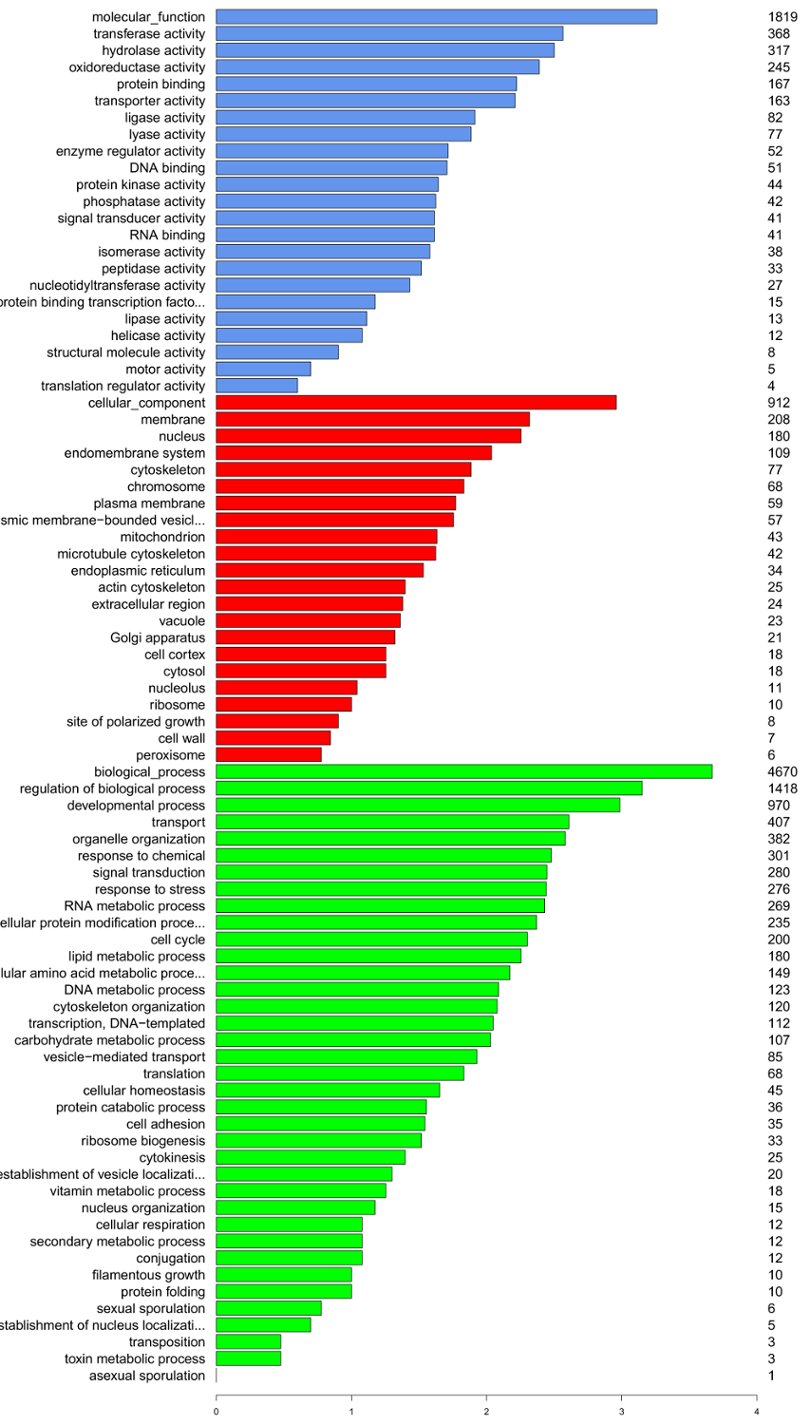
\includegraphics[width=4in]{./Chapter_Coelomomyces/img/Clat_aspergillus_GOPlot.png}
  \caption[\textit{C. lat} transcriptome GO term distribution]{Horizontal bar chart showing the distribution of \textit{Aspergillus} GO-Slim terms associated with the \textit{C. lativitattus} transcriptome. X axis is a logarithmic scale.}
  \label{fig:ChClat_GOPlot}
\end{figure}

% Opsin-GC fusion; chytrid cluster
\begin{figure}[hb]
  \centering
  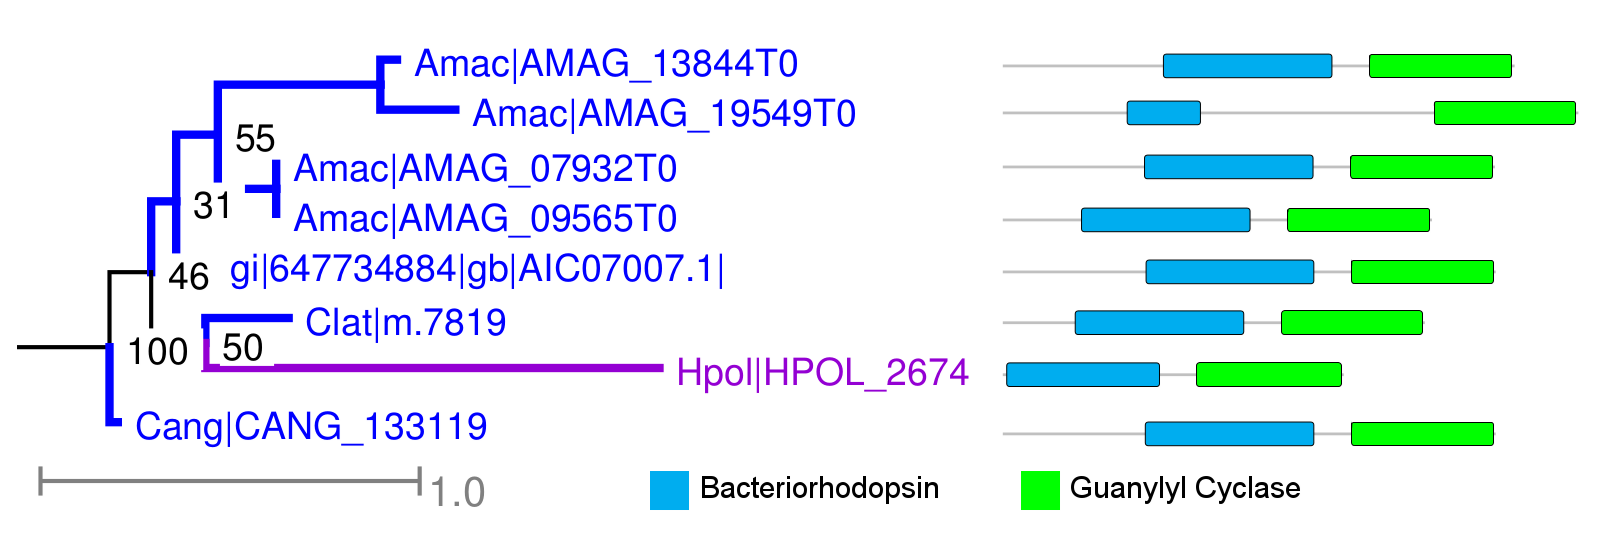
\includegraphics[width=4in]{./Chapter_Coelomomyces/img/OpsinGCFusion_chytridCluster.png}
  \caption[Opsin-GC fusion proteins]{A subset of bacterial opsin-guanylate cyclase fusion proteins. Proteins with similar architecture as described for \textit{B. emersonii} identified in Blastocladiomycete and Chytridiomycete proteomes, and \textit{C. lativitattus} transcriptome.}
  \label{fig:ChClat_OpsinGC}
\end{figure}

% Beta-carotene distribution
\begin{figure}[hb]
  \centering
  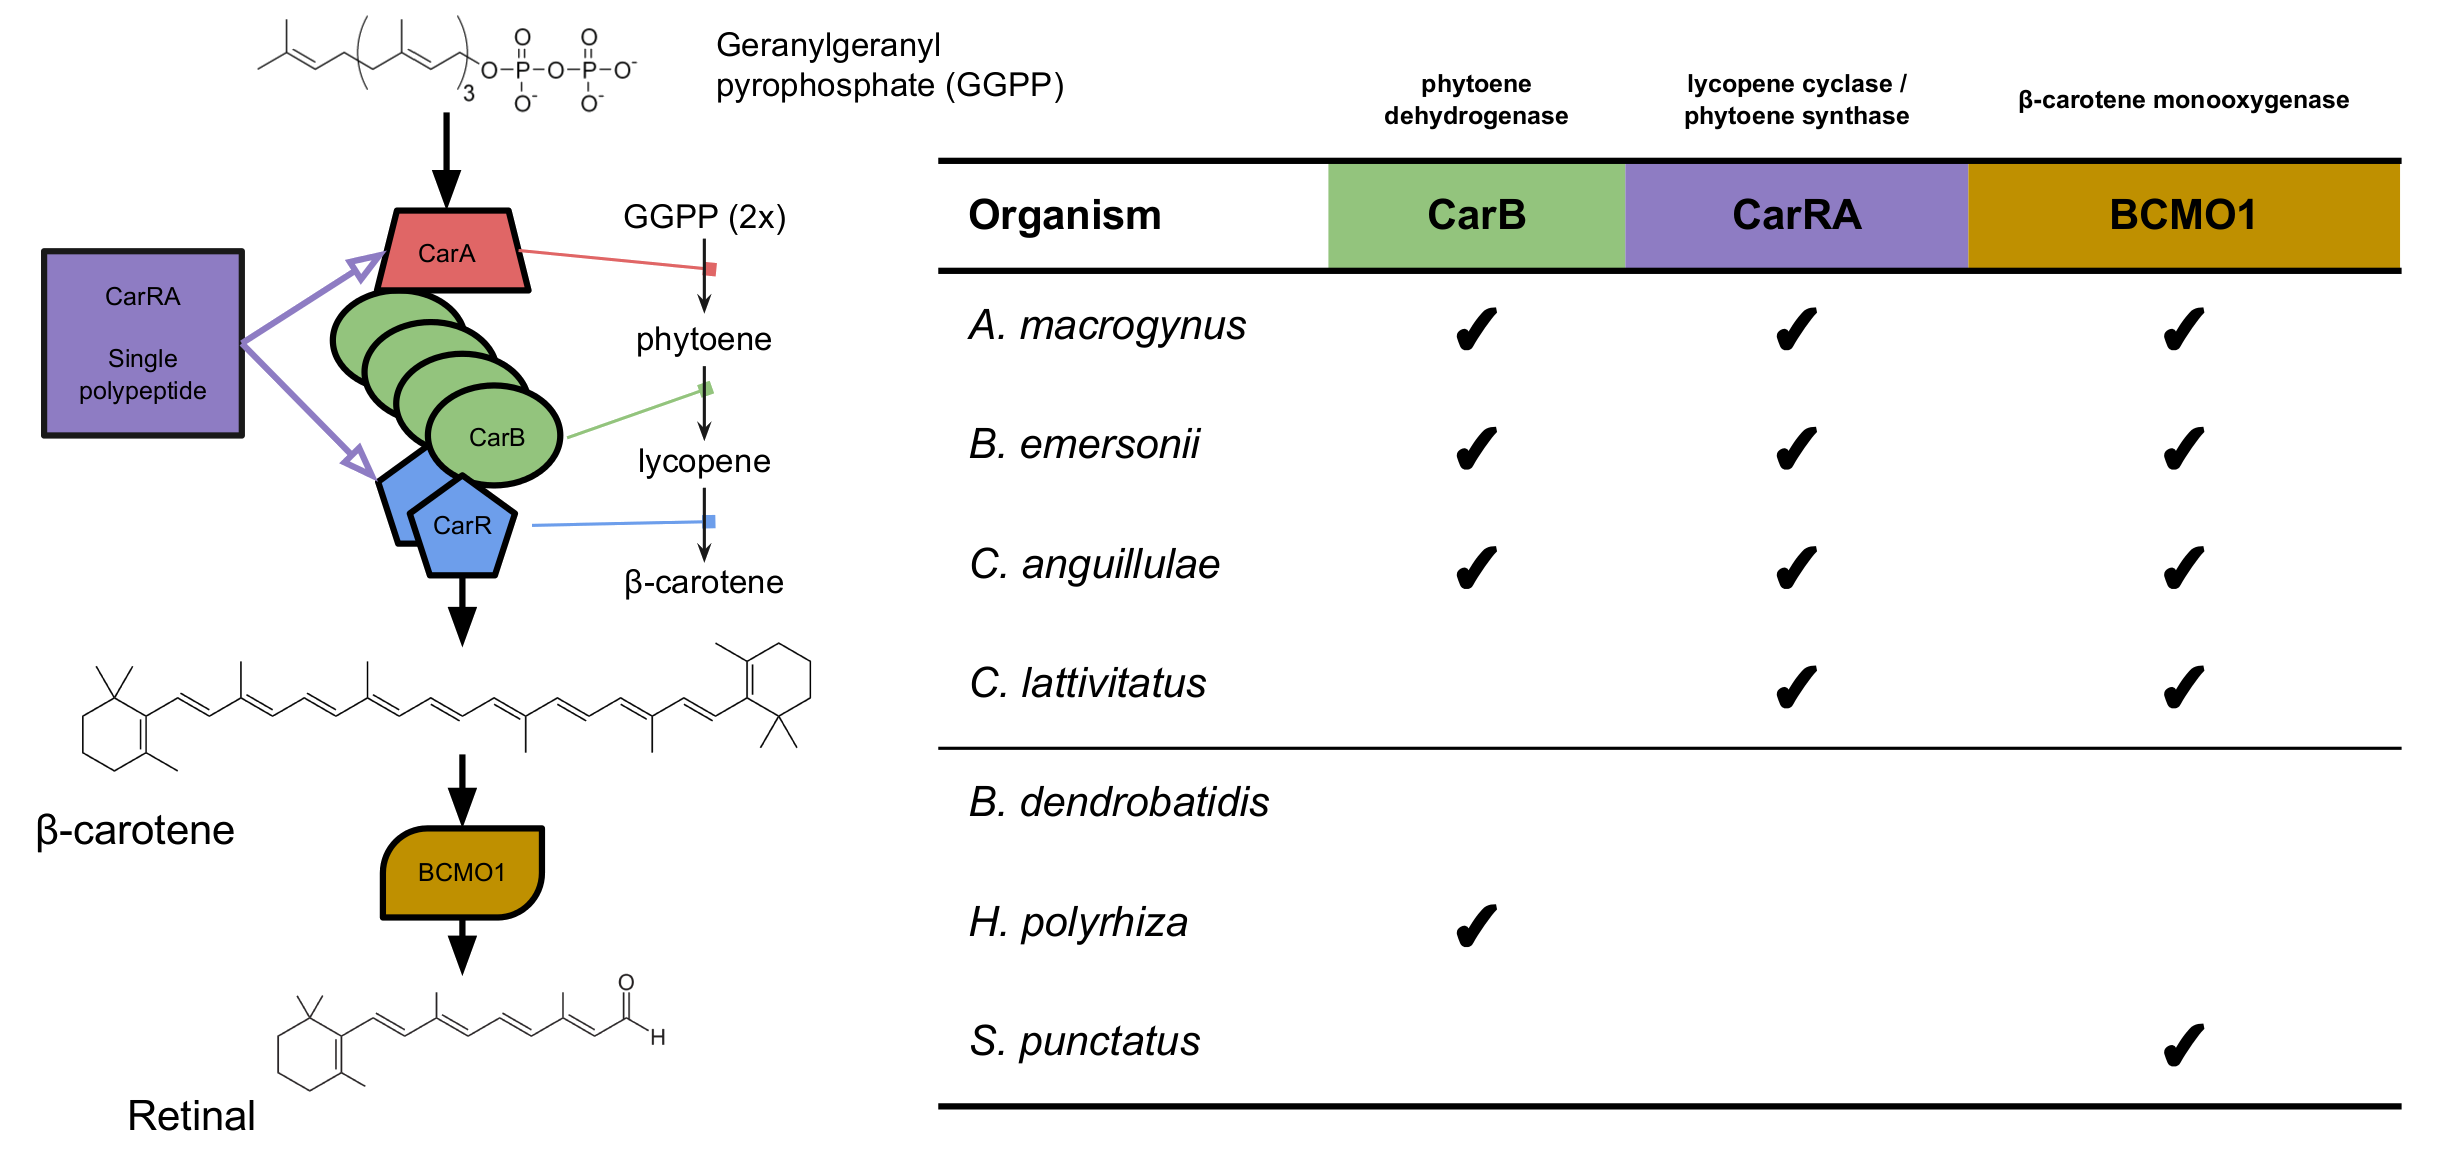
\includegraphics[width=4in]{./Chapter_Coelomomyces/img/Figure_bcaroPresenceAbsence.png}
  \caption[$\beta$-carotene enzyme presence / absence]{Presence and absence of $\beta$-carotene related proteins in species belonging to the Chytridiomycota and Blastocladiomycota.}
  \label{fig:ChClat_Bcaro}
\end{figure}

% PF00112 tree
\begin{figure}[hb]
  \centering
  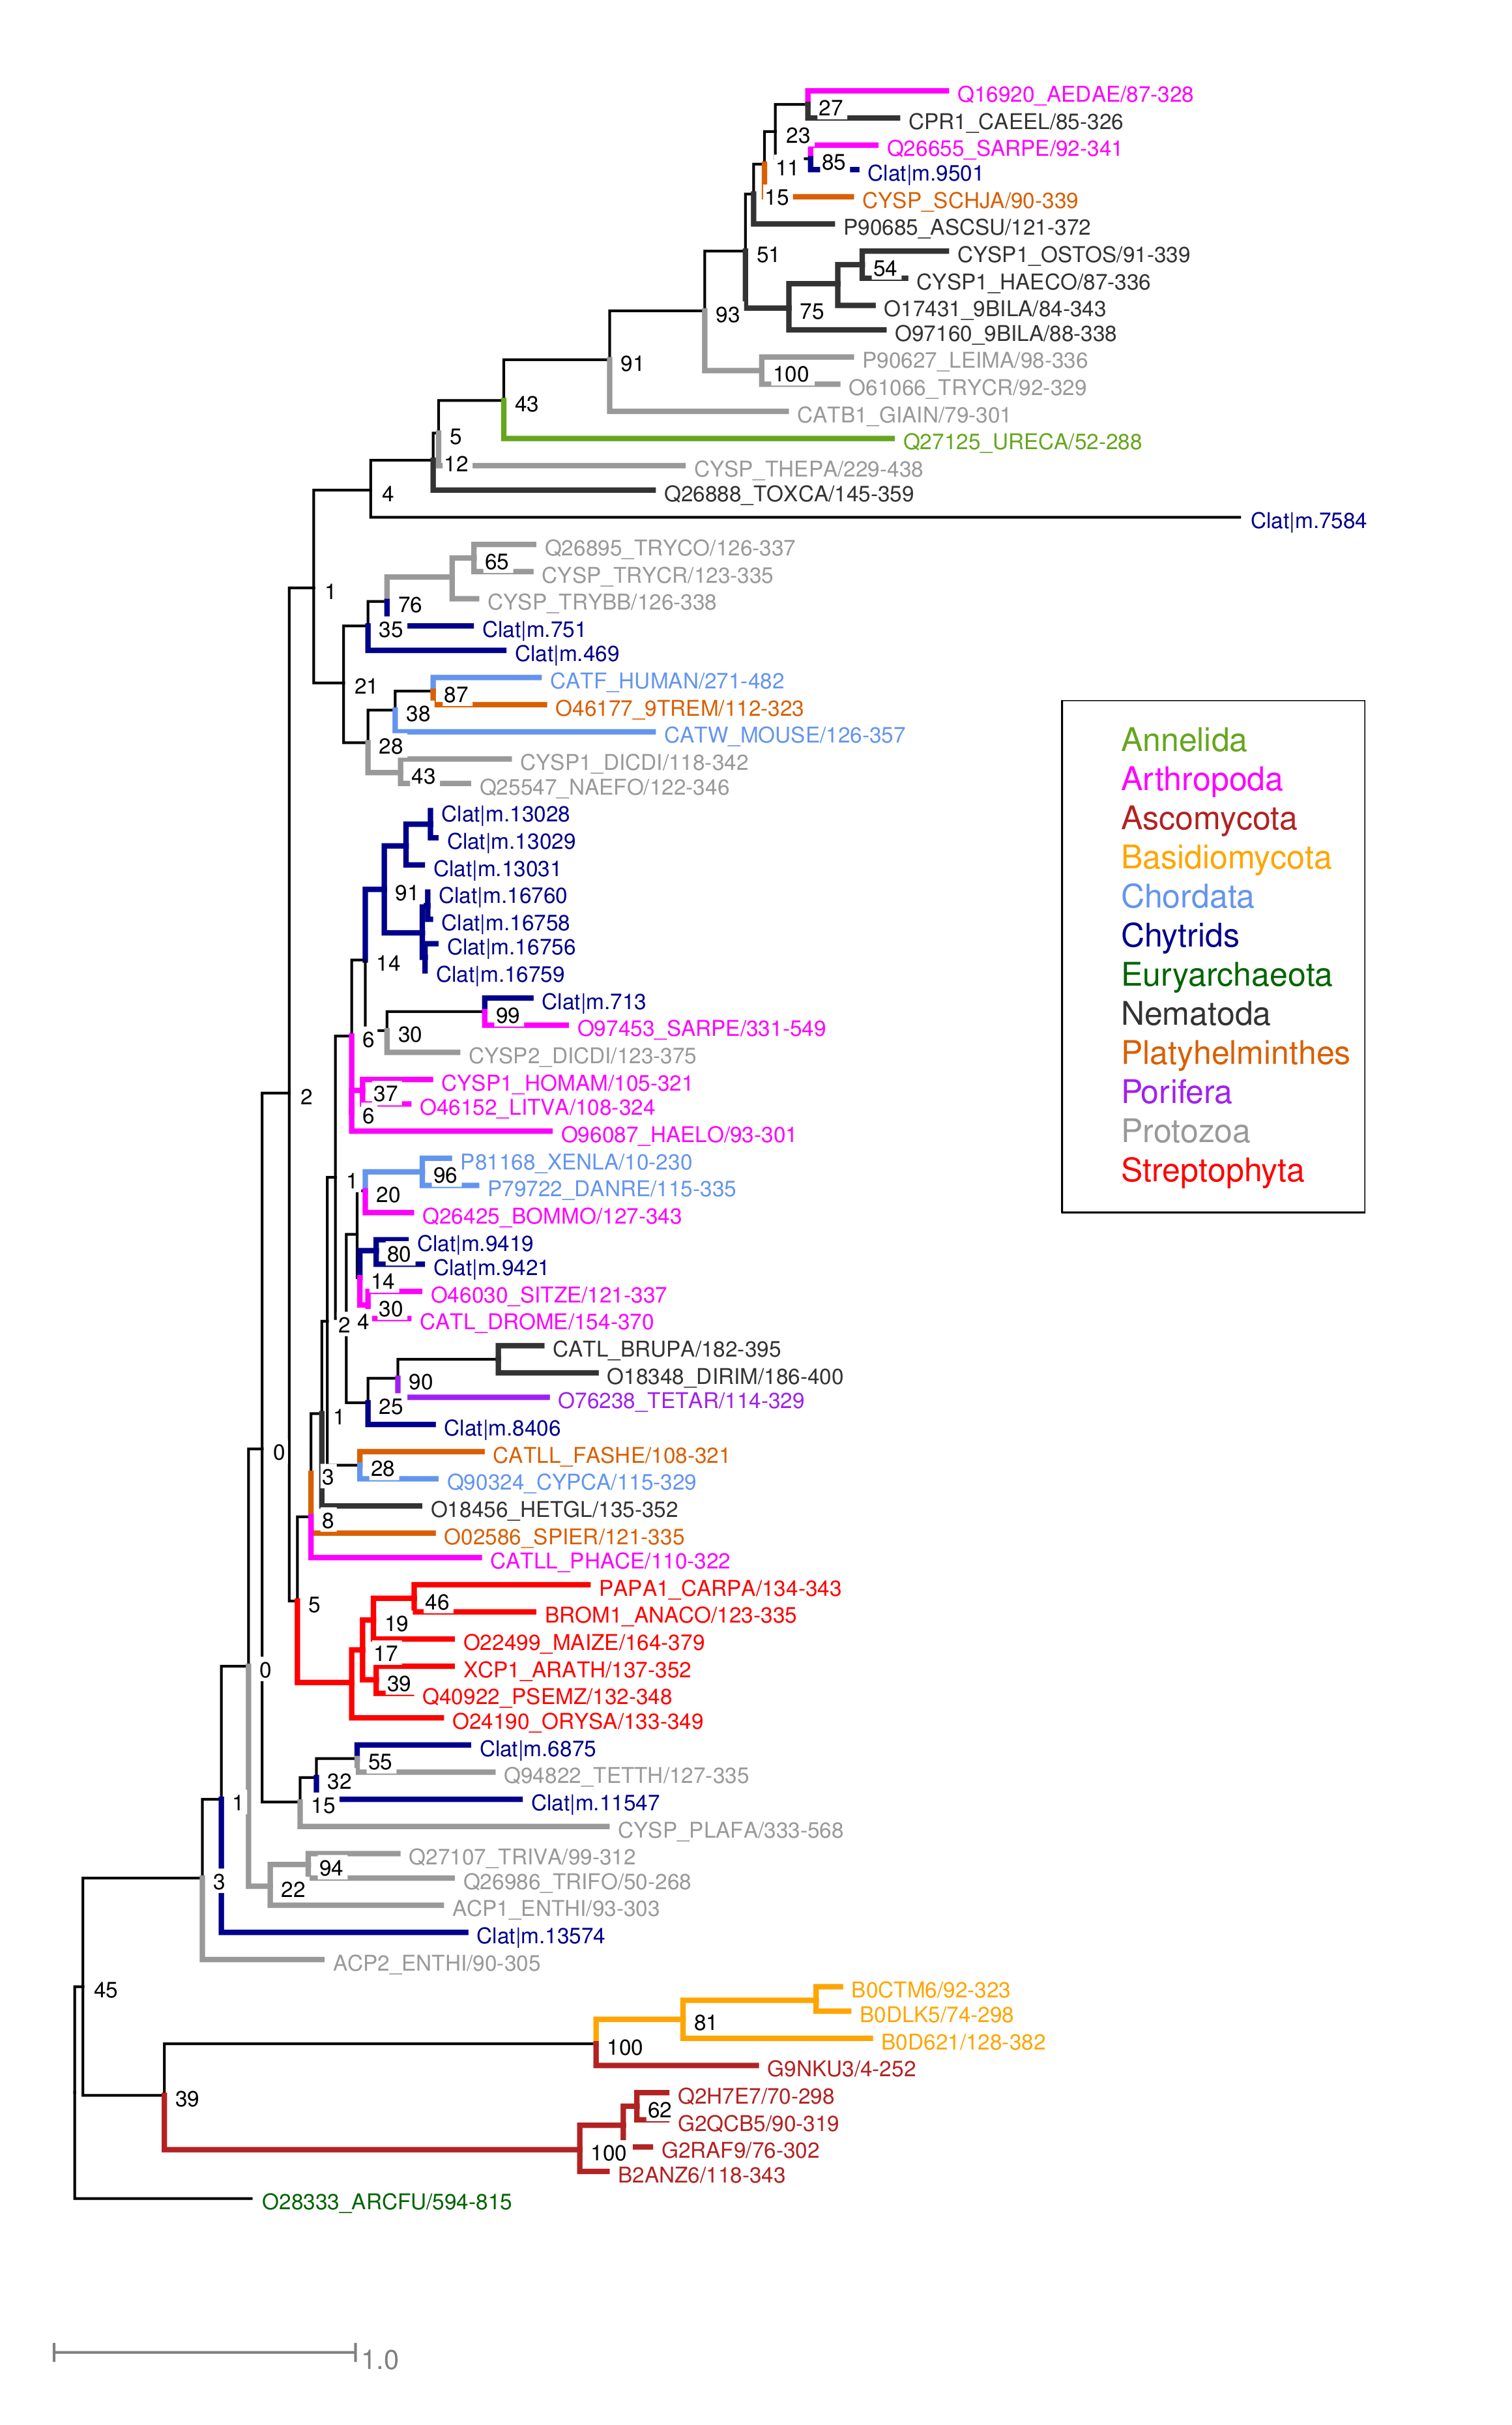
\includegraphics[width=4in]{./Chapter_Coelomomyces/img/PF00112_tree.png}
  \caption[PF00112 RAxML tree]{RAxML tree of select PF00112 seed sequences, unique \textit{C. lat} protein sequences, and sequences from Dikarya species.}
  \label{fig:ChClat_PF00112}
\end{figure}

% PF00089 tree
\begin{figure}[hb]
  \centering
  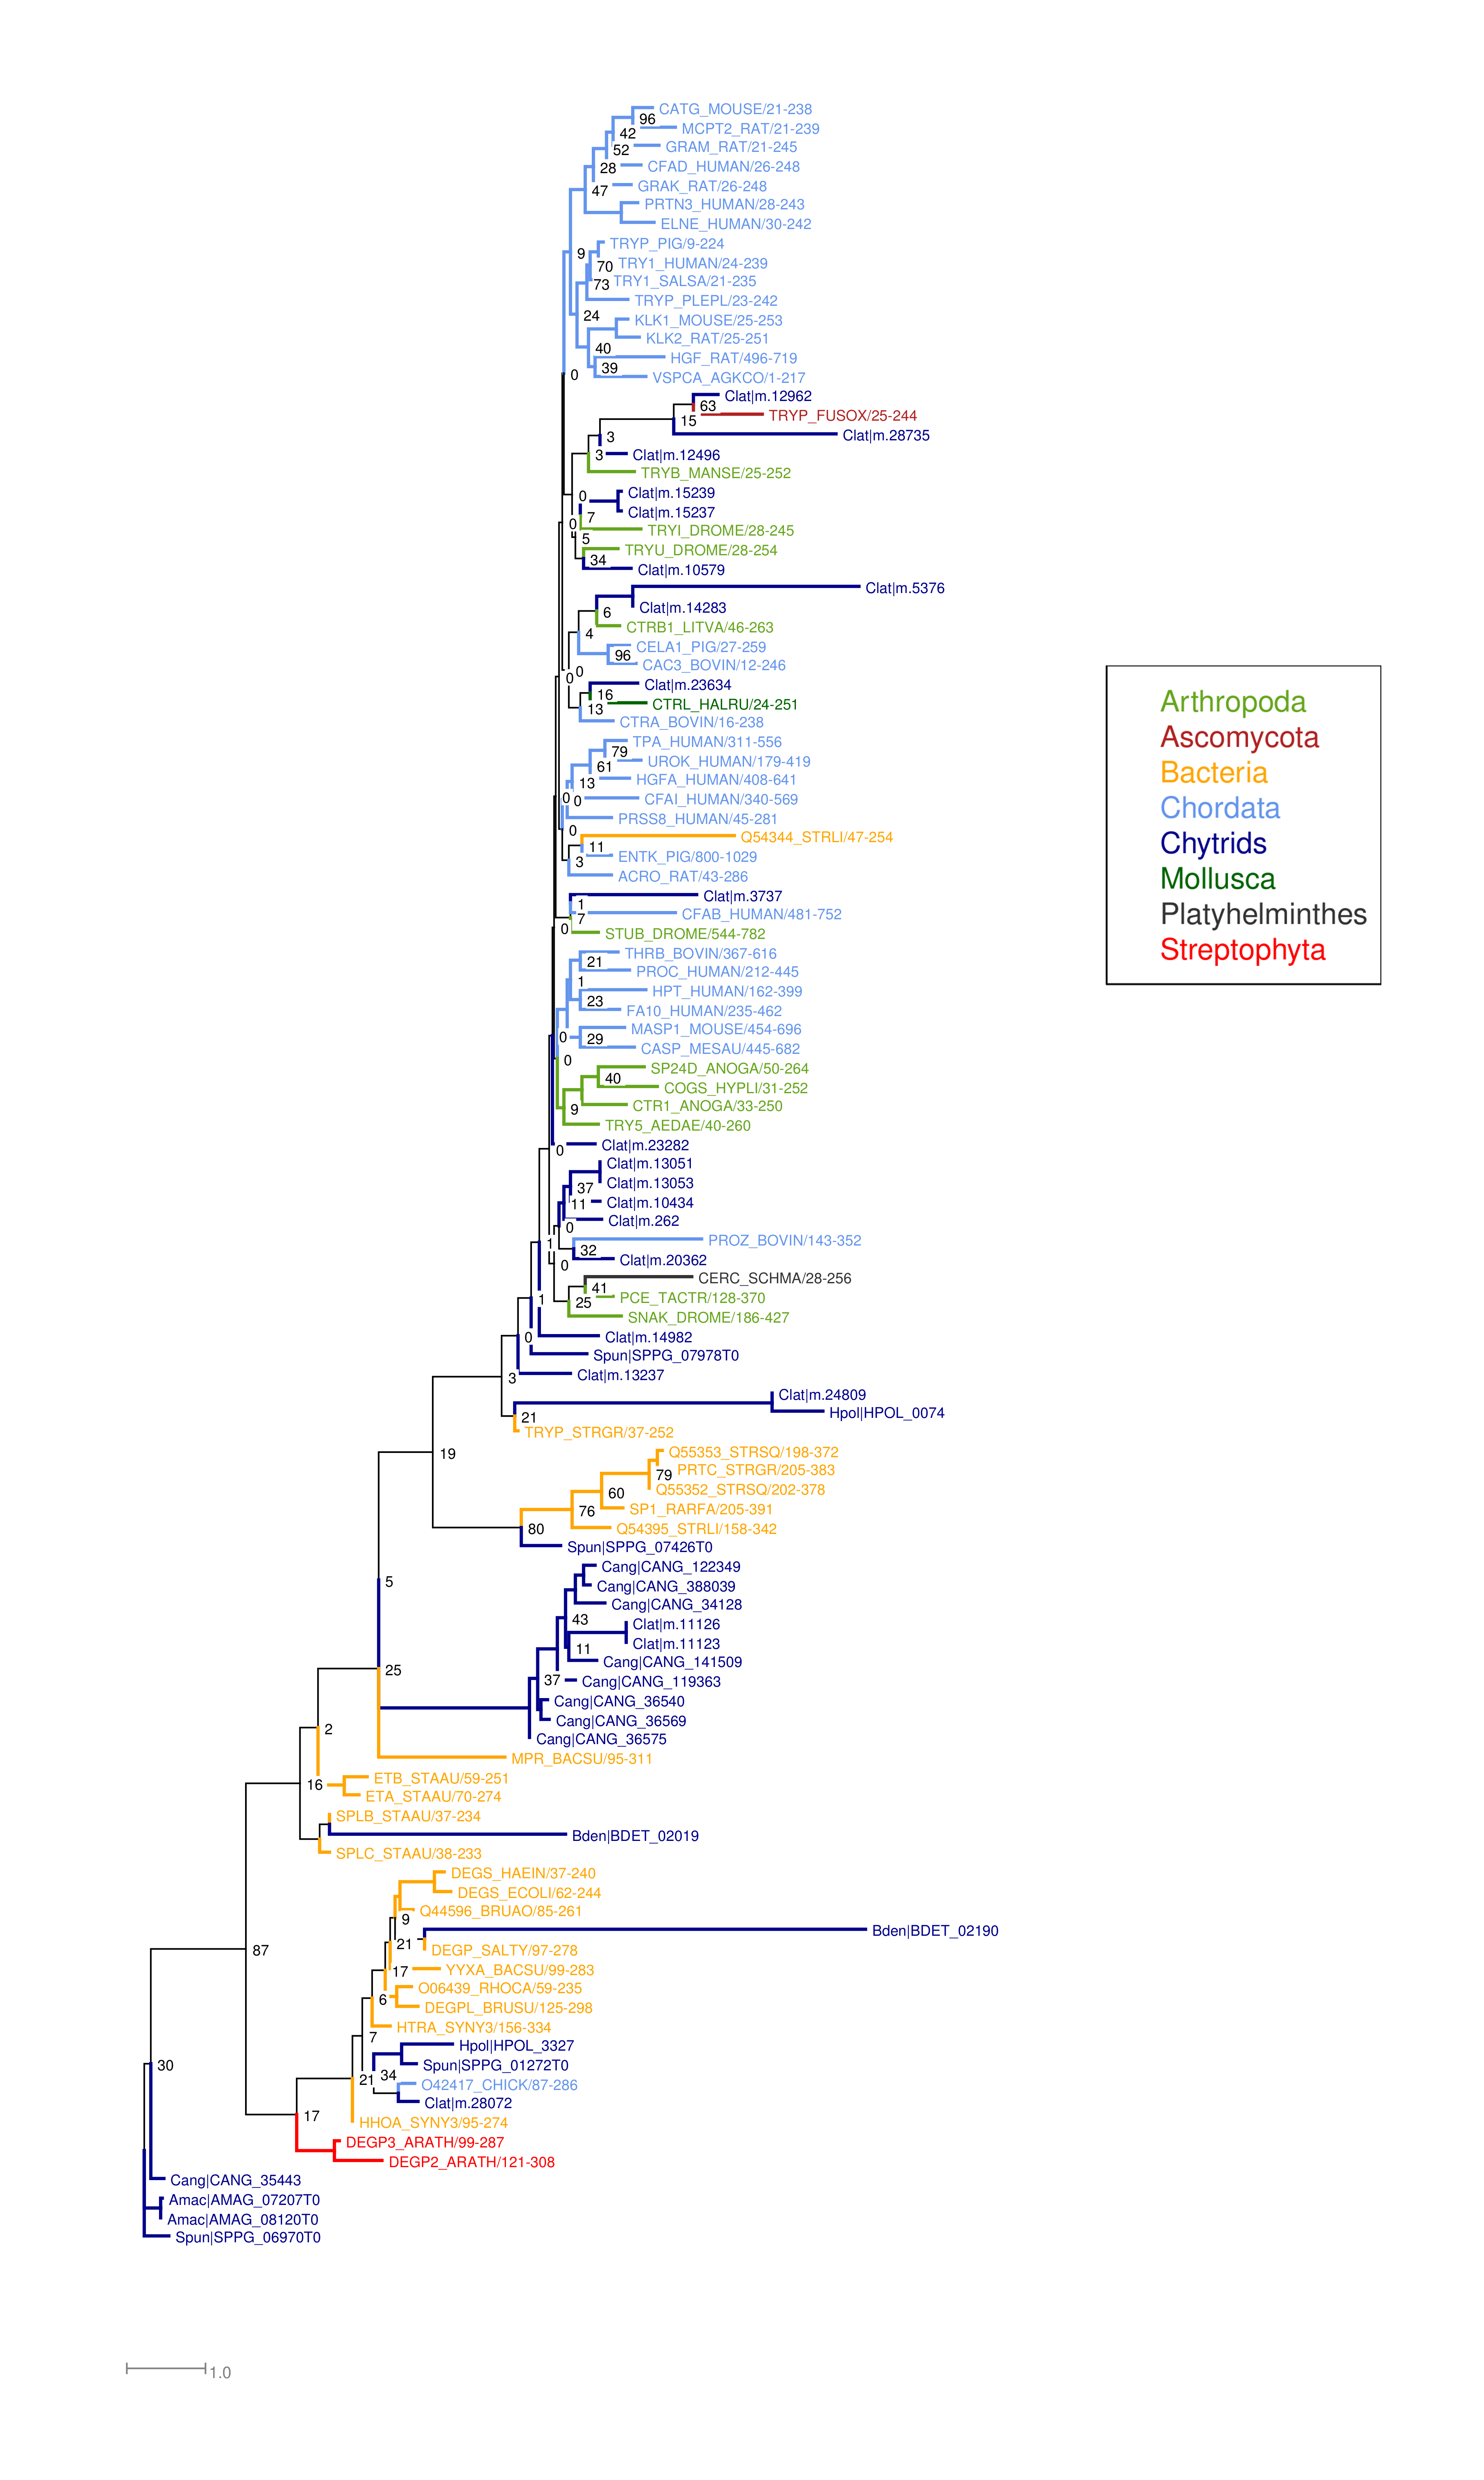
\includegraphics[width=4in]{./Chapter_Coelomomyces/img/PF00089_tree.png}
  \caption[PF00089 RAxML tree]{RAxML tree of select PF0089 seed sequences and unique \textit{C. lat} protein sequences}
  \label{fig:ChClat_PF00089}
\end{figure}

% 20HE receptor alignment
\begin{figure}[hb]
  \centering
  \begin{texshade}{./Chapter_Coelomomyces/dat/20HE_alignment.fa_aln}
    \threshold[80]{50}
    \shadingmode[allmatchspecial]{similar}
    \setends{1}{1..300}
    \hideconsensus
  \end{texshade}
  \caption[20HE alignment]{Alignment of \textit{D. melanogaster} EcR and putative 20HE receptors identified in \textit{C. lativittatus} }
  \label{fig:ChClat_20HEalign}
\end{figure}

%%%%%%%%%%%%%%%%%%%%%%%%%%%%%%%%%%%%%%%%%%%%%%%%%%%%%%%%%%%%%%%%%%%%%%%%%%%%%%%%%
%% Document: Thesis for PhD at UC Riverside                                    %%
%% Title: Investigating the evolution of environmental and biotic interactions %%
%%          in basal fungal lineages through comparative genomics              %%
%% Author: Steven Ahrendt                                                      %%
%%%%%%%%%%%%%%%%%%%%%%%%%%%%%%%%%%%%%%%%%%%%%%%%%%%%%%%%%%%%%%%%%%%%%%%%%%%%%%%%%
%% COELOMOMYCES TABLES %%
%%%%%%%%%%%%%%%%%%%%%%%%%

% latex table generated in R 3.0.1 by xtable 1.7-4 package
% Mon May 25 19:22:11 2015
\begin{table}[tbp]
\centering
\begin{tabular}{rlrrrrrr}
  \hline
\hline
 & Description & \emph{Clat} & \emph{Amac} & \emph{Cang} & \emph{Spun} & \emph{Bden} & \emph{Hpol} \\ 
  \hline
PF00069 & Pkinase & 297 & 409 & 185 & 354 & 404 & 149 \\ 
  PF00400 & WD40 & 211 & 1287 & 185 & 1710 & 1075 & 170 \\ 
  PF00076 & RRM 1 & 143 & 201 &  94 & 278 & 240 &  53 \\ 
  PF00153 & Mito carr & 119 & 222 &  42 & 294 & 231 &  49 \\ 
  PF00012 & HSP70 & 112 &  42 &  11 &  18 &  16 &   9 \\ 
  PF00118 & Cpn60 TCP1 &  93 &  22 &  11 &  20 &  31 &  10 \\ 
  PF00071 & Ras &  86 &  80 &  57 & 108 &  96 &  47 \\ 
  PF00270 & DEAD &  70 & 115 &  94 & 136 & 126 &  81 \\ 
  PF00036 & efhand &  67 &  27 &  49 &  60 &  68 &  30 \\ 
  PF00112 & Peptidase C1 &  65 &   0 &   1 &   0 &   0 &   0 \\ 
  PF01576 & Myosin tail 1 &  59 &   1 &  42 &   4 &   3 &  10 \\ 
  PF00004 & AAA &  58 & 128 & 121 & 134 & 135 &  93 \\ 
  PF00271 & Helicase C &  52 & 140 &  77 & 184 & 199 &  71 \\ 
  PF00227 & Proteasome &  52 &  26 &  16 &  28 &  43 &  19 \\ 
  PF01532 & Glyco hydro 47 &  52 &   2 &   3 &   8 &  12 &   8 \\ 
  PF07690 & MFS 1 &  50 & 144 &  57 & 120 &  69 &  36 \\ 
  PF02985 & HEAT &  50 &  34 &  64 &  56 & 136 &  58 \\ 
  PF00005 & ABC tran &  50 & 217 & 180 & 168 & 231 &  96 \\ 
  PF00009 & GTP EFTU &  48 &  79 &  80 &  92 &  48 &  54 \\ 
  PF00089 & Trypsin &  47 &   2 &   9 &   8 &   4 &   2 \\ 
   \hline
\hline
\end{tabular}
\caption[Top 20 PFAM domain counts]{Comparisions of counts of top 20 PFAM domains from \textit{C. lativittatus} as identified in other chytrids. Details for organism abbreviations can be found in appendix.} 
\label{tab:ChClat_PFAM}
\end{table}
% latex table generated in R 3.0.1 by xtable 1.7-4 package
% Mon May 25 19:22:11 2015
\begin{table}[tbp]
\centering
\begin{tabular}{rllllllrrrr}
  \hline
\hline
 & EMBLID & UniprotID & B..emersonii.Description & TopHitID & Top.hit.Description & Source.organism & X..Cov & E.val & X..ID & PMID \\ 
  \hline
1 & KJ468786 & A0A060GS52 & putative phytoene dehydrogenase & P54982 & phytoene desaturase & Phycomyces blakesleeanus NRRL 1555 &  85 & 0.00 &  53 & 9079885 \\ 
  2 & KJ468785 & A0A060GVE0 & putative lycopene cyclase / phytoene synthase & Q9UUQ6 & bifunctional lycopene cyclase/phytoene synthase & Mucor circinelloides f. lusitanicus &  93 & 0.00 &  33 & 10951210 \\ 
  3 & KJ468787 & A0A060GW07 & putative carotenoid dioxygenase & Q9I993 & Beta,beta-carotene 15,15'-monooxygenase & Gallus gallus &  51 & 0.00 &  27 & 10799297 \\ 
   \hline
\hline
\end{tabular}
\caption[BLASTP results for \textit{B. emersonii} $\beta$-carotene genes]{Top BLASTP hits against SwissProt for three \textit{B. emersonii} $\beta$-carotene metabolism genes. PMID references publications for SwissProt hit describing experimental verification of biological function} 
\label{tab:ChClat_BemeVerify}
\end{table}
% latex table generated in R 3.0.1 by xtable 1.7-4 package
% Mon May 25 19:22:11 2015
\begin{table}[tbp]
\centering
\begin{tabular}{rlll}
  \hline
\hline
 & KEGG.ID & Description & Sequences.used \\ 
  \hline
1 & K10027 & phytoene desaturase & 442 Bacterial proteins, 49 Archaeal proteins \\ 
  2 & K02291 & phytoene synthase & 6 Eukaryote proteins, 45 Plant proteins [excluded 49 Archaeal and 843 Bacterial proteins] \\ 
  3 & K00515 & beta-carotene 15,15'-monooxygenase & 64 Metazoan proteins [excluded 1 Archaeal protein] \\ 
   \hline
\hline
\end{tabular}
\caption[$\beta$-carotene HMM]{Sequences from KEGG used in generating HMMs for $\beta$-carotene metabolism searches} 
\label{tab:ChClat_KEGGHMM}
\end{table}
% latex table generated in R 3.0.1 by xtable 1.7-4 package
% Mon May 25 19:22:11 2015
\begin{table}[tbp]
\centering
\begin{tabular}{rrll}
  \hline
\hline
 & Cluster & Protein & Description \\ 
  \hline
1 & 1127 & Clat$|$m.15402 & 7tm\_1;PF00001 \\ 
  2 & 1127 & Clat$|$m.16182 & 7tm\_1;PF00001 \\ 
  3 & 1127 & Clat$|$m.18794 & 7tm\_1;PF00001 \\ 
  4 & 1127 & Clat$|$m.9338 & 7tm\_1;PF00001 \\ 
  5 & 1175 & Clat$|$m.12314 & K\_trans;PF02705 \\ 
  6 & 1175 & Clat$|$m.12319 & K\_trans;PF02705 \\ 
  7 & 1175 & Clat$|$m.12322 & K\_trans;PF02705 \\ 
  8 & 1176 & Clat$|$m.15582 & Grp1\_Fun34\_YaaH;PF01184 \\ 
  9 & 1176 & Clat$|$m.15583 & Grp1\_Fun34\_YaaH;PF01184 \\ 
  10 & 1176 & Clat$|$m.15584 & Grp1\_Fun34\_YaaH;PF01184 \\ 
  11 & 1177 & Clat$|$m.16070 & DUF3533;PF12051 \\ 
  12 & 1177 & Clat$|$m.16072 & DUF3533;PF12051 \\ 
  13 & 1177 & Clat$|$m.16075 & DUF3533;PF12051 \\ 
  14 & 1269 & Clat$|$m.11119 & UAA transporter;PF08449 \\ 
  15 & 1269 & Clat$|$m.11121 & UAA transporter;PF08449 \\ 
  16 & 1270 & Clat$|$m.12151 & -- \\ 
  17 & 1270 & Clat$|$m.12173 & -- \\ 
  18 & 1271 & Clat$|$m.8230 & -- \\ 
  19 & 1271 & Clat$|$m.8232 & -- \\ 
  20 & 1272 & Clat$|$m.12638 & -- \\ 
  21 & 1272 & Clat$|$m.12641 & -- \\ 
  22 & 1273 & Clat$|$m.14468 & Sodium:sulfate symporter;PF00939 \\ 
  23 & 1273 & Clat$|$m.14469 & Sodium:sulfate symporter;PF00939 \\ 
  24 & 1274 & Clat$|$m.14625 & -- \\ 
  25 & 1274 & Clat$|$m.14626 & -- \\ 
  26 & 1275 & Clat$|$m.4725 & NADH-Ubiquinone/plastoquinone;PF00361 \\ 
  27 & 1275 & Clat$|$m.8681 & NADH-Ubiquinone/plastoquinone;PF00361 \\ 
  28 & 1276 & Clat$|$m.4968 & Chitin synthase;PF03142 \\ 
  29 & 1276 & Clat$|$m.4970 & Chitin synthase;PF03142 \\ 
   \hline
\hline
\end{tabular}
\caption[orthoMCL short caption]{orthoMCL Long caption} 
\label{tab:ChClat_orthomcl}
\end{table}

% latex table generated in R 3.0.1 by xtable 1.7-4 package
% Mon May 25 19:22:11 2015
\begin{table}[tbp]
\centering
\begin{tabular}{rlllllr}
  \hline
\hline
 & OrfID & Type & UniProtKB.BLAST.match & InterPro & TMPred & FPKM \\ 
  \hline
1 & m.12730 & WC-1 & Neurospora crassa\verb|^|Q01371\verb|^|4e-43 & -- & -- & 2.37 \\ 
  2 & m.7819 & OpGC & Halobacterium sp. NRC-1\verb|^|P71411\verb|^|7.4e-07;Drosophila melanogaster\verb|^|Q8INF0\verb|^|8e-44 & PF01036\verb|^|32:241\verb|^|5.0e-37;PF00211\verb|^|355:533\verb|^|4.6e-51 & -- & 18.00 \\ 
  3 & m.9338 & Op & Danio rerio\verb|^|Q2KNE5\verb|^|3e-08 & PF10317\verb|^|21:205\verb|^|1.9e-7;PF00001\verb|^|50:355\verb|^|1.5e-17 & -- & 12.40 \\ 
  4 & m.15402 & Op & Apis mellifera\verb|^|Q17053\verb|^|8e-10 & PF00001\verb|^|36:341\verb|^|1.0e-21 & -- & 5.17 \\ 
  5 & m.16182 & Op & Cambarus hubrichti\verb|^|O18312\verb|^|1e-04 & PF00001\verb|^|14:255\verb|^|9.7e-13 & -- & 4.70 \\ 
  6 & m.18794 & Op & Limulus polyphemus\verb|^|P35360\verb|^|3e-10 & PF00001\verb|^|20:323\verb|^|5.9e-22 & -- & 1.62 \\ 
  7 & m.11198 & Op & Halobacterium sp. AUS-2\verb|^|P29563\verb|^|3e-30 & PF01036\verb|^|32:241\verb|^|5.0e-37 & -- & 1.54 \\ 
   \hline
\hline
\end{tabular}
\caption[\textit{C. lativittatus} photosensing proteins]{Predicted \textit{C. lativittatus} proteins associated with photosensing. PFAM Family definitions: PF13426, "PAS domain" [PAS\_9]; PF08447, "PAS fold" [PAS\_3]; PF00001, "7 transmembrane receptor (rhodopsin family)" [7tm\_1]; PF01036, "bacteriorhodopsin-like protein" [Bac\_rhodopsin]; PF10317, "Serpentine type 7TM GPCR chemoreceptor Srd" [7TM\_GPCR\_Srd]; PF00211, "Adenylate and Guanylate cyclase catalytic domain" [Guanylate\_cyc]} 
\label{tab:ChClat_photosensing}
\end{table}
% latex table generated in R 3.0.1 by xtable 1.7-4 package
% Mon May 25 19:22:11 2015
\begin{table}[tbp]
\centering
\begin{tabular}{rrllrrr}
  \hline
\hline
 & SVM.Score & UniprotKB.ID & Description & Identity & Alignment.Length & E.value \\ 
  \hline
Amac$|$AMAG\_17113T0 & -0.74 & Q9DBG3.1 & AP-2 complex subunit beta & 55.26 & 903 & 0.00 \\ 
  Amac$|$AMAG\_05862T0 & -0.61 & P00940.2 & Triosephosphate isomerase EC=5.3.1.1 & 58.06 & 248 & 0.00 \\ 
  Amac$|$AMAG\_12167T0 & -0.54 & P00940.2 & Triosephosphate isomerase EC=5.3.1.1 & 59.27 & 248 & 0.00 \\ 
  Amac$|$AMAG\_08758T0 & -0.19 & P46226.3 & Triosephosphate isomerase, cytosolic EC=5.3.1.1 & 59.84 & 249 & 0.00 \\ 
  Amac$|$AMAG\_10182T0 & -0.17 & P46226.3 & Triosephosphate isomerase, cytosolic EC=5.3.1.1 & 60.24 & 249 & 0.00 \\ 
  Amac$|$AMAG\_18542T0 & -0.16 & P48491.2 & Triosephosphate isomerase, cytosolic EC=5.3.1.1 & 58.19 & 177 & 0.00 \\ 
  Amac$|$AMAG\_16371T0 & 0.15 &  &  &  &  &  \\ 
  Amac$|$AMAG\_08832T0 & 0.17 & Q966L9.1 & ATP-dependent RNA helicase glh-2 EC=3.6.4.13 & 54.63 & 108 & 0.00 \\ 
  Amac$|$AMAG\_17977T0 & 0.21 &  &  &  &  &  \\ 
  Amac$|$AMAG\_16084T0 & 0.32 & P29141.1 & Minor extracellular protease vpr EC=3.4.21.- & 42.00 & 600 & 0.00 \\ 
  Amac$|$AMAG\_04496T0 & 0.34 & Q6H236.1 & Paternally-expressed gene 3 protein & 45.71 & 525 & 0.00 \\ 
  Amac$|$AMAG\_19066T0 & 0.76 &  &  &  &  &  \\ 
  Amac$|$AMAG\_20477T0 & 0.83 &  &  &  &  &  \\ 
  Amac$|$AMAG\_04749T0 & 1.33 &  &  &  &  &  \\ 
  Amac$|$AMAG\_03430T0 & 1.43 &  &  &  &  &  \\ 
  Cang$|$CANG\_48379 & -0.78 & Q06852.2 & Cell surface glycoprotein 1 & 29.47 & 431 & 0.00 \\ 
  Cang$|$CANG\_125451 & -0.68 & P58559.1 & Glyceraldehyde-3-phosphate dehydrogenase 3 EC=1.2.1.12 & 58.02 & 343 & 0.00 \\ 
  Cang$|$CANG\_33361 & -0.09 & P48494.3 & Triosephosphate isomerase, cytosolic EC=5.3.1.1 & 59.04 & 249 & 0.00 \\ 
  Cang$|$CANG\_38430 & 0.60 & P22105.3 & Tenascin-X & 39.67 & 673 & 0.00 \\ 
  Cang$|$CANG\_69396 & 0.94 &  &  &  &  &  \\ 
  Clat$|$m.10957 & -0.78 & P27393.1 & Collagen alpha-2(IV) chain & 63.61 & 665 & 0.00 \\ 
  Clat$|$m.22466 & -0.75 & Q6CJG5.2 & Triosephosphate isomerase EC=5.3.1.1 & 48.60 & 179 & 0.00 \\ 
  Clat$|$m.2165 & -0.68 & A7S7F2.1 & Bystin & 43.48 & 276 & 0.00 \\ 
  Clat$|$m.18806 & -0.68 & P48501.1 & Triosephosphate isomerase EC=5.3.1.1 & 56.19 & 226 & 0.00 \\ 
  Clat$|$m.13634 & -0.63 & Q90XG0.1 & Triosephosphate isomerase B EC=5.3.1.1 & 71.02 & 245 & 0.00 \\ 
  Clat$|$m.1572 & -0.58 & O09452.1 & Glyceraldehyde-3-phosphate dehydrogenase, chloroplastic EC=1.2.1.59 & 84.01 & 269 & 0.00 \\ 
  Clat$|$m.15929 & -0.52 & P07487.2 & Glyceraldehyde-3-phosphate dehydrogenase 2 EC=1.2.1.12 & 80.28 & 142 & 0.00 \\ 
  Clat$|$m.10361 & -0.46 & P20445.2 & Glyceraldehyde-3-phosphate dehydrogenase EC=1.2.1.12 & 61.34 & 238 & 0.00 \\ 
  Clat$|$m.18916 & -0.42 & P48501.1 & Triosephosphate isomerase EC=5.3.1.1 & 60.87 & 253 & 0.00 \\ 
  Clat$|$m.11233 & -0.30 & Q96UF2.1 & Glyceraldehyde-3-phosphate dehydrogenase 2 EC=1.2.1.12 & 68.82 & 279 & 0.00 \\ 
  Clat$|$m.4480 & -0.07 & O77458.1 & Triosephosphate isomerase EC=5.3.1.1 & 64.24 & 165 & 0.00 \\ 
  Clat$|$m.13062 & 0.52 & Q6BMK0.1 & Glyceraldehyde-3-phosphate dehydrogenase EC=1.2.1.12 & 74.52 & 157 & 0.00 \\ 
  Clat$|$m.745 & 0.90 & Q92824.4 & Proprotein convertase subtilisin/kexin type 5 EC=3.4.21.- & 36.65 & 562 & 0.00 \\ 
  Clat$|$m.16183 & 1.05 & P22105.3 & Tenascin-X & 51.01 & 545 & 0.00 \\ 
  Clat$|$m.13342 & 1.13 & Q92824.4 & Proprotein convertase subtilisin/kexin type 5 EC=3.4.21.- & 43.22 & 1025 & 0.00 \\ 
  Clat$|$m.11209 & 2.24 &  &  &  &  &  \\ 
  Bden$|$BDET\_06684 & -0.79 & Q5R2J2.1 & Glyceraldehyde-3-phosphate dehydrogenase EC=1.2.1.12 EC=2.6.99.- & 71.56 & 334 & 0.00 \\ 
  Bden$|$BDET\_05736 & -0.17 & P00939.1 & Triosephosphate isomerase EC=5.3.1.1 & 57.66 & 248 & 0.00 \\ 
  Bden$|$BDET\_05372 & -0.03 & Q95P23.1 & Enterin neuropeptides & 28.02 & 182 & 0.00 \\ 
  Bden$|$BDET\_01761 & 0.45 & Q9AVB0.1 & Lectin-B & 64.57 & 460 & 0.00 \\ 
  Bden$|$BDET\_00626 & 0.49 &  &  &  &  &  \\ 
  Bden$|$BDET\_00287 & 0.67 & Q9AVB0.1 & Lectin-B & 58.01 & 462 & 0.00 \\ 
  Bden$|$BDET\_02239 & 1.45 & P23253.1 & Sialidase EC=3.2.1.18 & 54.09 & 318 & 0.00 \\ 
  Bden$|$BDET\_00436 & 1.48 &  &  &  &  &  \\ 
  Bden$|$BDET\_03668 & 1.51 & Q63425.2 & Periaxin & 39.51 & 367 & 0.00 \\ 
  Bden$|$BDET\_06100 & 1.70 &  &  &  &  &  \\ 
  Hpol$|$HPOL\_4940 & -0.79 & P00940.2 & Triosephosphate isomerase EC=5.3.1.1 & 56.63 & 249 & 0.00 \\ 
  Hpol$|$HPOL\_4790 & -0.46 & O57479.3 & Glyceraldehyde-3-phosphate dehydrogenase EC=1.2.1.12 EC=2.6.99.- & 75.61 & 328 & 0.00 \\ 
  Hpol$|$HPOL\_4769 & -0.24 & P52041.2 & 3-hydroxybutyryl-CoA dehydrogenase EC=1.1.1.157 & 40.00 &  80 & 0.00 \\ 
  Hpol$|$HPOL\_2513 & -0.14 & Q1ZXD6.1 & Probable serine/threonine-protein kinase roco5 EC=2.7.11.1 & 32.78 & 180 & 0.00 \\ 
  Spun$|$SPPG\_01012T0 & -0.68 & P30741.2 & Triosephosphate isomerase EC=5.3.1.1 & 61.60 & 250 & 0.00 \\ 
  Spun$|$SPPG\_08522T0 & -0.47 & Q6ZRI0.3 & Otogelin & 31.26 & 531 & 0.00 \\ 
  Spun$|$SPPG\_00685T0 & -0.15 & Q5H8C1.3 & FRAS1-related extracellular matrix protein 1 & 33.98 & 1292 & 0.00 \\ 
  Spun$|$SPPG\_01988T0 & 0.05 &  &  &  &  &  \\ 
   \hline
\hline
\end{tabular}
\caption[FAADB short caption]{FAADB Long caption} 
\label{tab:ChClat_FAADB}
\end{table}
% latex table generated in R 3.0.1 by xtable 1.7-4 package
% Mon May 25 19:22:11 2015
\begin{table}[tbp]
\centering
\begin{tabular}{rlrll}
  \hline
\hline
 & Coverage & E.val & X..Identity & Description \\ 
  \hline
Q5E9B6.1 & 40\% & 0.00 & 28\% & Liver X receptor alpha [Bos taurus] \\ 
  Q13133.2 & 40\% & 0.00 & 28\% & Liver X receptor alpha [Homo sapiens] \\ 
  Q62685.1 & 40\% & 0.00 & 28\% & Liver X receptor alpha [Rattus norvegicus] \\ 
  Q9Z0Y9.3 & 40\% & 0.00 & 28\% & Liver X receptor alpha [Mus musculus] \\ 
  P55055.2 & 40\% & 0.00 & 28\% & Liver X receptor beta [Homo sapiens] \\ 
   \hline
P49880.2 & 36\% & 0.00 & 28\% & 20-hydroxy-ecdysone receptor [Aedes aegypti] \\ 
  P49883.1 & 42\% & 0.00 & 24\% & 20-hydroxy-ecdysone receptor [Manduca sexta] \\ 
  P49881.1 & 42\% & 0.00 & 24\% & 20-hydroxy-ecdysone receptor [Bombyx mori] \\ 
  P34021.1 & 36\% & 0.00 & 26\% & 20-hydroxy-ecdysone receptor [Drosophila melongaster] \\ 
  O18531.2 & 36\% & 0.00 & 27\% & 20-hydroxy-ecdysone receptor [Lucilia cuprina] \\ 
  P49882.1 & 36\% & 0.00 & 25\% & 20-hydroxy-ecdysone receptor [Chironomus tentans] \\ 
   \hline
\hline
\end{tabular}
\caption[BLASTP hits for \textit{C. lat} m.10080]{BLASTP results using \textit{C. lativittatus} ORF m.10080 as a query against SwissProt database. Top five hits are to liver X receptors (LXRs) from various mammalian species. The next siz hits are only those which were to 20-hydroxy-ecdysone receptors, all of which are from insects} 
\label{tab:ChClat_LBD}
\end{table}


%%%%%%%%%%%%%%%%%%%%%%
% INHIBITION CHAPTER %
%%%%%%%%%%%%%%%%%%%%%%
%%%%%%%%%%%%%%%%%%%%%%%%%%%%%%%%%%%%%%%%%%%%%%%%%%%%%%%%%%%%%%%%%%%%%%%%%%%%%%%%%
%% Document: Thesis for PhD at UC Riverside                                    %%
%% Title: Investigating the evolution of environmental and biotic interactions %%
%%          in basal fungal lineages through comparative genomics              %%
%% Author: Steven Ahrendt                                                      %%
%%%%%%%%%%%%%%%%%%%%%%%%%%%%%%%%%%%%%%%%%%%%%%%%%%%%%%%%%%%%%%%%%%%%%%%%%%%%%%%%%
% INHIBITION CHAPTER %
%%%%%%%%%%%%%%%%%%%%%%
\chapter{Growth suppression properties of the Chytridiomycete \textit{Homolaphlyctis polyrhiza} JEL142}
\label{chap:Hp_inhibition}
\section{Introduction}
Interactions between microorganisms are facilitated by biological signals. These include proteins, small molecules, and various chemical compounds, either bound to the cell surface or secreted into the environment. Many of these compounds can be classified as secondary metabolites: chemicals not required for growth or development of the organism. \\
\indent Resource competition likely plays a role in the evolution of natural antifungal production \cite{Vicente2003}. Secretion by an organism in a resource-limited environment of secondary metabolites which also happen to negatively impact neighboring organisms would confer a selective advantage upon the producer.\\
\indent There are many fungal pathogens of economically important crops (eg. \textit{Fusarium graminearum}, \textit{Magnaporthe grisea}, \textit{Ashbya gossypii}) and humans (eg. \textit{Aspergillus fumigatus}). Research into new natural antifungal treatment is increasingly important as certain pathogenic fungi become progressively resistant to current, conventionally synthesized antifungal drugs (see reviews by Bossche et al. in 1998\nocite{Bossche1998}, Kontoyiannis and Lewis in 2002\nocite{Kontoyiannis2002}, and Pfaller in 2012\nocite{Pfaller2012}. \\
\indent There are numerous examples of fungi as potent producers of these types of compounds, including toxins \cite{Kokkonen2010}, antimicrobials \cite{Wiemann2014}, and plant hormone mimics \cite{Howlett2006}. The thrust of research into fungal-derived secondary metabolites focuses on Ascomycete and Basidiomycete fungi due to their diverse product types \cite{Berdy2012}.\\
\subsection{Background of chytrids and Hp}
However, flagellated fungal lineages, commonly known as "chytrids", are a relatively understudied group, both in general and in this regard specifically. These lineages, closest to the Fungal-Animal divergence and sister to other fungal groups, are known for having a uniflagellate, zoosporic stage in their life cycles and fulfil crucial ecological roles such as terrestrial decomposition. Additionally, several species are pathogenic (eg \textit{Batrachochytrium dendrobatidis} \cite{Longcore1999}, \textit{Coelomomyces} spp. \cite{Couch1972}, and \textit{Rozella allomycis} \cite{James2013}), with intracellular and/or extracellular lifestages. Comparative genomic analyses have identified a variety of degradation enzymes in their genomes, but the full extent of competition-based secondary metabolite production has yet to be explored. It is likely that these organisms have evolved mechanisms for mediating chemical interactions with other organisms, and therefore could present a potentially valuable source of novel antifungal compounds.\\
\indent \textit{Homolaphlyctis polyrhiza} (\textit{Hp}) is a non-pathogenic member of the Chytridiomycota and is most closely related to the amphibian pathogen \textit{B. dendrobatidis} (\textit{Bd}). The specific isolate, \textit{Hp} JEL 142, has been used previously in phylogenetic studies of chytrids \cite{James2000,James2006,Letcher2008} and was provided a formal name in 2011 \cite{Longcore2011}. A draft 454 genome assembly was produced in that same year for comparative insights into pathogenicity of \textit{Bd} \cite{Joneson2011}.\\
\indent This isolate was collected in Maine, USA from a 1.7 ha oligotrophic and fishless lake with a pH of 4.6 \cite{Davis1994,Rhodes1995}. It was cultured using onionskin bait and isolated into pure culture on mPmTG nutrient agar. Its overall morphology is typical of members of the Rhizophydiales, but phylogenetic reanalysis prompted the description of a novel genus and species \cite{Longcore2011}.\\
\indent While working with \textit{Hp} in the Stajich lab for the phototaxis and protein expression experiments described in Chapter~\ref{chap:RhodStruct}, I made the discovery of accidental contamination of \textit{Hp} plates by \textit{N. crassa}. Specifically, I first noticed the distinctive zone created by \textit{N. crassa} hyphae growing near \textit{Hp} sporangia (illustrated in Figure~\ref{ChInhib_NcChytrid}A. I also had previously observed this type of contamination on plates of related Chytridiomycetes \textit{Bd} and \textit{Sp}, which did not demonstrate this inhibitory effect when co-cultured with \textit{N. crassa}.\\
\indent This property of \textit{Hp} is reliable and reproducible. This chapter, therefore, describes the experimental and computational work towards identification and characterization of a compound responsible for hyphal growth suppression of \textit{N. crassa} by \textit{Hp}. This represents the first study of \textit{Hp} in this context and presents novel findings about microbial interactions within early branching fungal lineages. Significant help, specifically concerning media prep and general strain maintenance, was provided by undergraduate students in the Stajich lab Na Jeong and Sapphire Ear, and visiting student in the Research Experience for Undergraduates (REU) program Spencer Swansen.\\
\section{Methods}
\subsection{Fungal strains and maintenance}
Cultures of \textit{Homolaphlyctis polyrhiza} JEL142, \textit{Operculomyces laminatus} JEL223, \textit{Rhizoclosmatium hyalinus} JEL800, and \textit{Obelidium mucronatum} JEL802 were individually maintained on mPmTG [peptonized milk (0.4 g/L), tryptone (0.4 g/L), dextrose (2 g/L)], \textit{Batrachochytrium dendrobatidis} JEL423 cultures were maintained on 1\% Tryptone [tryptone (10 g/L), dextrose (3.2 g/L)], and \textit{Spizellomyces punctatus} SW-1 cultures were maintained on PmTG [peptonized milk (0.5 g/L), tryptone (1 g/L), dextrose (5 g/L)]. All chytrid cultures were maintained at room temperature (approx. 23$^{\circ}$C. Unless otherwise specified, all experiments using chytrids were carried out using the specific media described above for each species. Motile chytrid zoospores, when required, were obtained from actively growing (ie 2-4 day old) plates by flooding and subsequently (after 30-45 minutes at room temperature) collecting 2-4 mls of sterile di H$_{2}$O. Sporangia samples for inoculation were obtained by removing a block (approx. 1 cm$^{2}$) of agar containing actively-growing chytrid sporangia.\\
\indent Vogel's minimal medium (VM) (Davis1970) was used for vegetative growth of \textit{Neurospora crassa} FGSC 2489, \textit{Neurospora discreta} FGSC 8579 and \textit{Neurospora tetrasperma} FGSC 2508. \textit{Neurospora crassa} kinase/phosphotase mutants (Table~\ref{tab:kinase}; \cite{Park2011}) were maintained on VM + Hygromycin and grown similarly to \textit{N. crassa} WT strains. \textit{Trichoderma reesei} FGSC 10290 , \textit{Phycomyces blakesleeanus}, and \textit{Ashbya gossypii} cultures were maintained on PDA media [potato dextrose agar (39 g/L)] at 28$^{\circ}$C, 20$^{\circ}$C, and 30$^{\circ}$C, respectively. \textit{Aspergillus nidulans} FGSC A4 cultures were maintained on minimal media [dextrose (10 g/L), nitrate salts (50 mL/L), Trace elements (1 ml/L)], at 28$^{\circ}$C. \textit{Saccharomyces cerevisiae} strains MAU99 and AH109 were maintained on YPDA [yeast extract (10 g/L), peptone (20 g/L), dextrose (20 g/L), adenine sulfate (0.003\%)] media at 35$^{\circ}$C. \textit{Corpinopsis cinerea} FGSC 9003 cultures were maintained on YPD media at 37$^{\circ}$C.  Plates and slants of 1\% tryptone, PmTG, mPmTG, VM, YPD, and PDA media included 1\% agar. Plates and slants of MM included 1.8\% agar. Plates and slants of YPDA included 2\% agar.\\
\subsection{Bioactivity on solid media}
To assess the breadth of fungal species susceptible to \textit{Hp} sporangia, \textit{Hp} was individually co-cultured on mPmTG media with the variety of fungi described above. A block of agar containing active \textit{Hp} sporangia was added to mPmTG plate, flushed with sterile diH$_{2}$O, and incubated for 48h, at which point they were inoculated at a single point with 1x10$^{\circ}$ \textit{Neurospora} conidia in diH$_{2}$O. For \textit{Neurospora} experiments, plates were left to grow for an additional 24 - 48 hrs.\\
\indent Similarly, for other fungi (which are much slower growing than \textit{Neurospora}), \textit{Hp} and the target fungus were inoculated at the same time on an mPmTG solid media plate.\\
\subsection{Bioactivity in liquid media}
Figure~\ref{fig:ChInhib_filtrateProtocol} illustrates the general protocol for obtaining aliquots of filter-sterilized\textit{Hp}-conditioned media ("filtrate") to test for bioactivity. For small quantities, initial preparations (in triplicate) were constructed by adding eight blocks of agar containing actively-growing \textit{Hp} sporangia, each approximately 1cm$^{2}$ to 10 ml of liquid mPmTG. To initially help determine if the compound was being constitutivelyu-produced or a response mechanism, a second preparation was made identically to the one just described, to which an additional 0.5 $\mu$l of a 100 $\mu$l  \textit{N. crassa} conidial suspension was added. To help control for potential nutrient depletion by \textit{N. crassa} in this second preparation, a third preparation contained eight mPmTG agar blocks with no \textit{Hp} sporangial growth in 10 ml mPmTG, and 0.5 $\mu$l of a 100 $\mu$l \textit{N. crassa} conidial suspension. These preparations were left to incubate at room temperature for 72hrs, at which point the total filtrate was obtained by passing each individual replicate through a 0.22 $\mu$m syringe filter into a 50 ml conical tube. All replicates for a given treatment were pooled after filtration. \\
\indent Scaled up experiments were performed in a similar manner: twenty blocks of agar containing \textit{Hp} sporangia were added to 50 ml of mPmTG media, and filtered using a 0.22 $\mu$m syringe filter.\\
\indent For temperature assays, the filtrate from each small scale preparation was subsequently divided into eight 2 ml aliquots (in duplicate) to test for bioactivity over three separate experiments. The control sample was left undisturbed and uninoculated throughout the experiment. Another sample was inoculated with 2x10$^{6}$ conidia but otherwise untreated. The filtrate was subjected to six different temperature treatments to test its thermostability: -80$^{\circ}$C (30 min), -20$^{\circ}$C (1 hr), 4$^{\circ}$C (1 hr), 28$^{\circ}$C (1 hr), 65$^{\circ}$C (1 hr), and 90$^{\circ}$C (30 min). Each experimental treatment was inoculated with 2x10$^{\circ}$6 conidia. These temperature treatments were allowed to return to room temperature prior to inoculation.\\
\indent To test the sensitivity of \textit{Bd} to \textit{Hp}, 3 ml of the filtrate from the large scale preparation was used as an incubation medium for one blcok of 1\% Tryptone agar containing actively growing \textit{Bd} sporangia. Similarly, 3 ml of mPmTG media was used as a positive control. These preparations were incubated for 96h at room temperature to allow for potential zoospore production and release. After 96h, the suspension was mixed briefly and 1 ml was added to mPmTG plates, while another 1 ml was added to 1\% Tryptone plates. The plates were incubated at room temperature for a maximum of 14d and photographed periodically.\\
\subsection{Reassembly and annotation}
\textit{Hp} sporangia material was collected by scraping plates with sterile spatulas. Material was ground using bead-beating methods, and DNA obtained using extraction methods. A DNAseq Illumina library was prepared using the NEBNext Ultra DNA library kit and submitted to the University of California, Riverside Genomics Institute for Integrateve Genomic Biology (IIGB) core facility for MiSeq Illumina HT sequencing.\\
\subsection{Secretome and small-metabolite screen}
A comparative analysis of putative small metabolite and secretome composition in chytrids was performed using antiSMASH \cite{Blin2013}, and a predictive workflow optimized for fungi described by \cite{Min2010}.\\
\indent Scripts used in these analyses are located at https://github.com/sahrendt0/Scripts/tree/master/Inhibition\_scripts.\\
\subsection{Temperature and pH growth assays}
To compare to the assays described in \cite{Piotrowski2004}, \textit{Hp} was grown at a range of temperatures: 18$^{\circ}$C, 23$^{\circ}$C, 25$^{\circ}$C, 28$^{\circ}$C, and 30$^{\circ}$C. Briefly, a 15 ml mPmTG inoculum was incubated at 23$^{\circ}$C for 1 week. 1 ml of culture was used to inoculate 30 ml of mPmTG in 50 ml conical tubes. \\
\indent Similarly, \textit{Hp} and \textit{Bd} were grown at a range of pHs by preparing mPmTG and 1\% Tryptone media at different pH levels: 4.0, 5.0, 6.0, 6.8, 8.0, and 9.0.\\
\section{Results}
\subsection{The physiology of \textit{Hp} suggests that it is more tolerant of environmental stresses than \textit{Bd}}
To assess whether or not the observed growth suppression effect was the result of acidification of the local environment, \textit{Hp} was cultured on plates augmented with bromophenol blue or phenol red. After 96h growth, neither plates changed color, indicating that \textit{Hp} sporangia do not decrease the pH of mPmTG media below 6.8. However, phenol red plates which were additionally inoculated with \textit{N. crassa} did change from red to yellow in the areas around \textit{N. crassa} hyphae, suggesting that \textit{N. crassa} acidifies mPmTG media to below pH 6.8. This effect is not observed in bromophenol blue plates, suggesting that the final pH lies between 6.8 and 4.6.\\
\indent To get a sense of the environmental tolerances of \textit{Hp} compared to \textit{Bd}, these two species were individually cultured in liquid media (mPmTG and 1\% Tryptone, respectively) prepared at different pHs, ranging from 4.0 to 9.0. The average OD$_{450}$, a measure of cell density, of \textit{Hp} at low pH (4 and 5) was 0.037 and 0.068 respectively, which was higher than that for \textit{Bd} (0.001 and 0.004 respectively). This suggests that \textit{Hp} is more tolerant of acidic environments than \textit{Bd} (Figure~\ref{fig:ChInhib_HpBdpHTemp}A). Similarly, \textit{Hp} and \textit{Bd} were grown at temperatures ranging from 18$^{\circ}$C to 30$^{\circ}$C, and the OD$_{450}$ assessed during a 21-day period (Figure~\ref{fig:ChInhib_HpBdpHTemp}B). Taken together, these results suggest that \textit{Hp} has a higher tolerance for environmental changes than \textit{Bd}. This finding isn’t terribly surprising given that this isolate was obtained from an acidic lake \cite{Longcore2011}.\\
\subsection{\textit{Hp} inhibition is unique among the chytrids and broadly active against other fungal species}
Our initial observations were repeatable, and under controlled circumstances, we were able to demonstrate that \textit{Hp} sporangia are reliably and repeatedly capable of inhibition of \textit{N. crassa} vegetative growth on solid mPmTG media (Figure~\ref{fig:ChInhib_NcraChytrid}A). The related species, \textit{Bd} and \textit{Sp}, do not demonstrate any inhibitory activity (Figure~\ref{fig:ChInhib_NcraChytrid}B and C). Additional Chytridiomycota species (\textit{Operculomyces laminatus} JEL 223, \textit{Rhizoclosmatium hyalinus} JEL 800, and \textit{Obelidium mucronatum} JEL 802) do not inhibit hyphal growth of \textit{N. crassa} (Figure~\ref{fig:ChInhib_NcraChytrid}D-F), providing additional support that this behavior is unique to \textit{Hp}. \\
\indent This phenomenon is not the result of any thigmotropism-related response or object avoidance type behavior in \textit{N. crassa}, as hyphae of \textit{N. crassa} are not inhibited by an agar block lacking \textit{Hp} sporangia (Figure~\ref{fig:ChInhib_NcAvoidance}).\\
\indent To determine if the sensitivity to \textit{Hp} sporangia was unique to \textit{N. crassa}, we screened a panel of fungi from among the Ascomycota, Basidiomycota, and Zygomycota. Figure~\ref{fig:ChInhib_HpOtherFungi}A recapitulates our previous observations about \textit{N. crassa}, while Figure~\ref{fig:ChInhib_HpOtherFungi}B and C demonstrate, respectively, that vegetative hyphal growth of \textit{N. discreta} and \textit{N. tetrasperma} can also be suppressed by the presence of \textit{Hp} sporangia.
\indent Within the Ascomycota, but outside of the genus Neurospora, \textit{Trichoderma reesei} (Sordariomycetes; Hypocreales; Hypocreaceae), \textit{Aspergillus nidulans} (Eurotiomycetes; Eurotiales; Trichocomaceae), and \textit{Ashbya gossypii} (Saccharomycetes; Saccharomycetales; Saccharomycetaceae) are all completely sensitive to \textit{Hp} (Figure~\ref{fig:ChInhib_HpOtherFungi}D-F, respectively). \\
\indent Within the Basidiomycota, \textit{Coprinopsis cinerea} (Agaricomycetes; Agaricales; Psathyrellaceae) is completely sensitive to \textit{Hp} sporangia (Figure~\ref{fig:ChInhib_HpOtherFungi}G). Growth of members of the order Mucorales had mixed sensitivities. \textit{Phycomyces blakesleeanus} (Mucorales; Phycomycetaceae) was completely sensitive to \textit{Hp} sporangia, yet \textit{Rhizopus oryzae} (Mucorales; Mucoraceae) appeared to be insensitive (Figure~\ref{fig:ChInhib_HpOtherFungi}H \& I, respectively). Despite a possibly limited panel of ten fungi, the broadly observed pattern of sensitivity suggests that the responsible compound has a generalized mechanism of action.\\
\indent Additionally, the growth in \textit{Hp} conditioned media filtrate of two strains of yeast (\textit{Saccharomyces cerevisiae} MAU99 and AH109) and \textit{E. coli} DH5$\alpha$ suggested that this filtrate inhibited liquid growth of these organisms, and also provides evidence that the antimicrobial properties of \textit{Hp} extend to bacteria as well (Figure~\ref{fig:ChInhib_HpYeastEcoli}).\\
\subsection{Liquid filtrate screening suggests a non-protein compound is responsible for bioactivity}
We were interested in obtaining a sample of bioactive liquid, on which we could perform chemical profiling to isolate a responsible compound. To test for bioactivity, \textit{Hp} cultured in liquid mPmTG media for a period of 72 hrs and subsequently filter-sterilized, producing “conditioned media” to which \textit{N. crassa} conidia was reintroduced. \\
\indent This conditioned media, obtained from \textit{Hp} and absent of all sporangia, retains the same inhibitory properties against \textit{N. crassa} observed with \textit{Hp} sporangia on solid agar plates (Figure~\ref{ChInhib_FilterTempAssay}A). Additionally, conditioned media derived from "Hp alone" and "Hp+Nc" preparations (Prep 1 and 2, Figure S3) were indistinguishable from one another in their effects on \textit{N. crassa} growth. \\
\indent The stability of the conditioned media was tested at seven different temperatures, ranging from -80$^{\circ}$C to 90$^{\circ}$C. The conditioned media retained bioactivity between -20$^{\circ}$C and 60$^{\circ}$C (Figure~\ref{fig:ChInhib_FilterTempAssay}D-E), but was ineffective after treatment of -80$^{\circ}$C and 90$^{\circ}$C (Figure~\ref{fig:ChInhib_FilterTempAssay}F-G). \textit{N. crassa} has no problem growing in fresh mPmTG media (Figure~\ref{fig:ChInhib_FilterTempAssay}H). Additionally, the conditioned media was ineffective if left sterile at room temperature for a period of 96h, and subsequently inoculated with \textit{N. crassa} conidia.\\
\indent After treatment of 100 mg/ml of Proteinase K, the conditioned media was no less effective at inhibition of N. crassa hyphal growth than untreated media (not shown or pull up figure / possibly take a week to repeat this).\\
\subsection{Secretome + antiSMASH analyses, coupled with improved genome assembly and annotation predicts a few unique secondary metabolite gene clusters with potential relevance}
Secretome prediction made using workflow from \cite{Min2010} (Figure 8). \\
\indent Secondary metabolite clusters were predicted using antiSMASH \cite{Blin2013} (Figure 9).\\
\indent Several unique proteins were found to be related to terpene synthases, and these were unique to Hp when compared to other Chytridiomycota and Blastocladiomycota species.\\
\indent Make a tree from these enzymes.\\
\subsection{Genome reassembly and reannotation}
\subsection{Miscellaneous}
\subsubsection{N. crassa hyphal tip morphology}
<Figure 3>\\
\subsubsection{Kinase mutant screen}
In order to address potential mechanisms of action for this behavior, we randomly assayed 2 N. crassa phosphotase and 17 kinase mutants from \cite{Park2011}. All were found to be inhibited by growing sporangia of H. polyrhiza (Table~\ref{tab:ChInhib_Kinase}).\\
\section{Discussion}
This study was an attempt to characterize a startling and unexpected observation: actively growing H. polyrhiza sporangia inhibit the vegetative, hyphal growth of N. crassa. The findings demonstrate that i) H. polyrhiza is unique among surveyed chytrids in its ability to inhibit filamentous growth of N. crassa, ii) the interaction is not limited to N. crassa but is broadly active against a number of Ascomycete, Basidiomycete, and Zygomycete species, and iii) in silico secondary metabolite analysis suggests a terpene synthase-related enzyme as a possible candidate based on observed unique expansion of genes.\\
\indent H. polyrhiza, an aquatic, non-parasitic member of the Chytridiomycota isolated from a lake in the northeastern United States, and N. crassa, a filamentous, multicellular, non-parasitic fungus primarily observed on decaying plant matter, are unlikely to come in specific contact with one another in the environment, so this response was presumed to be a non-specific interaction. The results from the broad fungal species screen support this presumption, and it appears that H. polyrhiza is active against a multitude of fungal species.\\
\indent Compared with other chytrid isolates we assayed, \textit{Hp} stands alone in its antifungal properties. Although the described basal lineages represent only 2\% of all described fungi, and the estimated diversity of these lineages is presumed high, this is the first time an interaction of this type has been described in any of these lineages. While it is possible that this behavior is not unique to this specific \textit{Hp} isolate, a more exhaustive assay of chytrid isolates is necessary to elaborate on this hypothesis.\\
\indent The observation that conditioned media derived from "Hp alone" and "Hp+Nc" preparations were indistinguishable from one another in their effects on \textit{N. crassa} growth suggests that the compound is being constitutively produced from H. polyrhiza and is not a response to a fungal competitor. Analysis of the transcriptome would be beneficial and would in theory easily identify any constitutively active genes in the sporangia life stage, from which this compound is expected to originate.\\
\indent The liquid compound profiling suggests that the compound is not protein-based. Filter-sterilized conditioned media was subjected to temperatures of -80$^{\circ}$C, -20$^{\circ}$C, 4$^{\circ}$C, 23$^{\circ}$C, 28$^{\circ}$C, 65$^{\circ}$C, and 90$^{\circ}$C, which are temperatures which would be expected during routine storage and/or shipping processes. With the exception of -80$^{\circ}$C and 90$^{\circ}$C, treatment at these temperatures did not negatively impact the growth suppression properties of the filtered conditioned media.\\
\indent We performed both in silico secretome and secondary metabolite screens using the previously published 454-based H. polyrhiza genome. The secondary metabolite screen in particular provided a rough idea of candidate enzymes which were expanded in \textit{H. polyrhiza}.\\
\indent Taken together, these data suggest that the compound is a constitutively-produced secondary metabolite compound with broadly specific activity. Its mechanism of action is unknown, as are its chemical structure and related biosynthetic pathway(s). Near term future work will necessarily focus on chemical profiling of bioactive spent media filtrate to generate a working hypothesis for the chemical nature of the product. A starting point for this research is provided in the form of in silico genomic and transcriptomic research. Finally, it is worth noting that the relative ease with which this discovery was made speaks to the necessity for further research into these basal lineages, of which intimate genomic and biochemical knowledge is lacking.

%%%%%%%%%%%%%%%%%%%%%%%%%%%%%%%%%%%%%%%%%%%%%%%%%%%%%%%%%%%%%%%%%%%%%%%%%%%%%%%%%
%% Document: Thesis for PhD at UC Riverside                                    %%
%% Title: Investigating the evolution of environmental and biotic interactions %%
%%          in basal fungal lineages through comparative genomics              %%
%% Author: Steven Ahrendt                                                      %%
%%%%%%%%%%%%%%%%%%%%%%%%%%%%%%%%%%%%%%%%%%%%%%%%%%%%%%%%%%%%%%%%%%%%%%%%%%%%%%%%%
%% INHIBITION FIGURES %%
%%%%%%%%%%%%%%%%%%%%%%%%
\begin{figure}[hb]
  \centering
  \includegraphics[width=4in]{./Chapter_Inhibition/img/Nc_HpBdSp_otherChytrids.png}
  \caption[Inhibition appears unique to \textit{Hp} among other chytrids]{\textit{Batrachochytrium dendrobatidis} JEL 423 (\textit{Bd}), the closest relative of \textit{Hp}, is well known as a global emerging pathogen of amphibians and is the causative agent for recent worldwide amphibian decline. \textit{Spizellomyces punctatus} SW-1 (\textit{Sp}) is a soil saprobe and is not known to be pathogenic. A) \textit{Hp} cultured with \textit{N. crassa} produces a cleared zone. B) \textit{Bd}, C) \textit{Sp}, D) \textit{Operculomyces laminatus} JEL 223, E) \textit{Rhizoclosmatium hyalinus} JEL 800, F) \textit{Obelidium mucronatum} JEL 802 do not display this property. Black scale bars = 1mm. Black arrowheads illustrate location of chytrid sporangia.}
  \label{fig:ChInhib_NcraChytrid}
\end{figure}

\begin{figure}[hb]
  \centering
  \includegraphics[width=4in]{./Chapter_Inhibition/img/HpvsOtherFungi.png}
  \caption[Inhibition is not specific to \textit{N. crassa}]{A selection of fungal species from the Ascomycota, Basidiomycota, and Mucorales were assayed for sensitivity against \textit{Hp} sporangia. A) \textit{Neurospora crassa} (Sordariomycetes; Sordariales; Sordariaceae), B) \textit{Neurospora tetrasperma}, C) \textit{Neurospora discreta}, D) \textit{Trichoderma reesei} (Sordariomycetes; Hypocreales; Hypocreaceae), E) \textit{Aspergillus nidulans} (Eurotiomycetes; Eurotiales; Trichocomaceae), F) \textit{Coprinopsis cinerea} (Agaricomycetes; Agaricales; Psathyrellaceae), G) \textit{Ashbya gossypii} (Saccharomycetes; Saccharomycetales; Saccharomycetaceae), H) \textit{Phycomyces blakesleeanus} (Mucorales; Phycomycetaceae), and I) \textit{Rhizopus oryzae} (Mucorales; Mucoraceae). Scale bars for A-C,H-I = 1mm. Scale bars for D-G = 5mm. Black arrowheads in A-C,H-I indicate \textit{Hp} sporangia. White arrowheads in A-G indicate blocks of agar with active \textit{Hp} sporangia.}
  \label{fig:ChInhib_HpOtherFungi}
\end{figure}

\begin{figure}[hb]
  \centering
  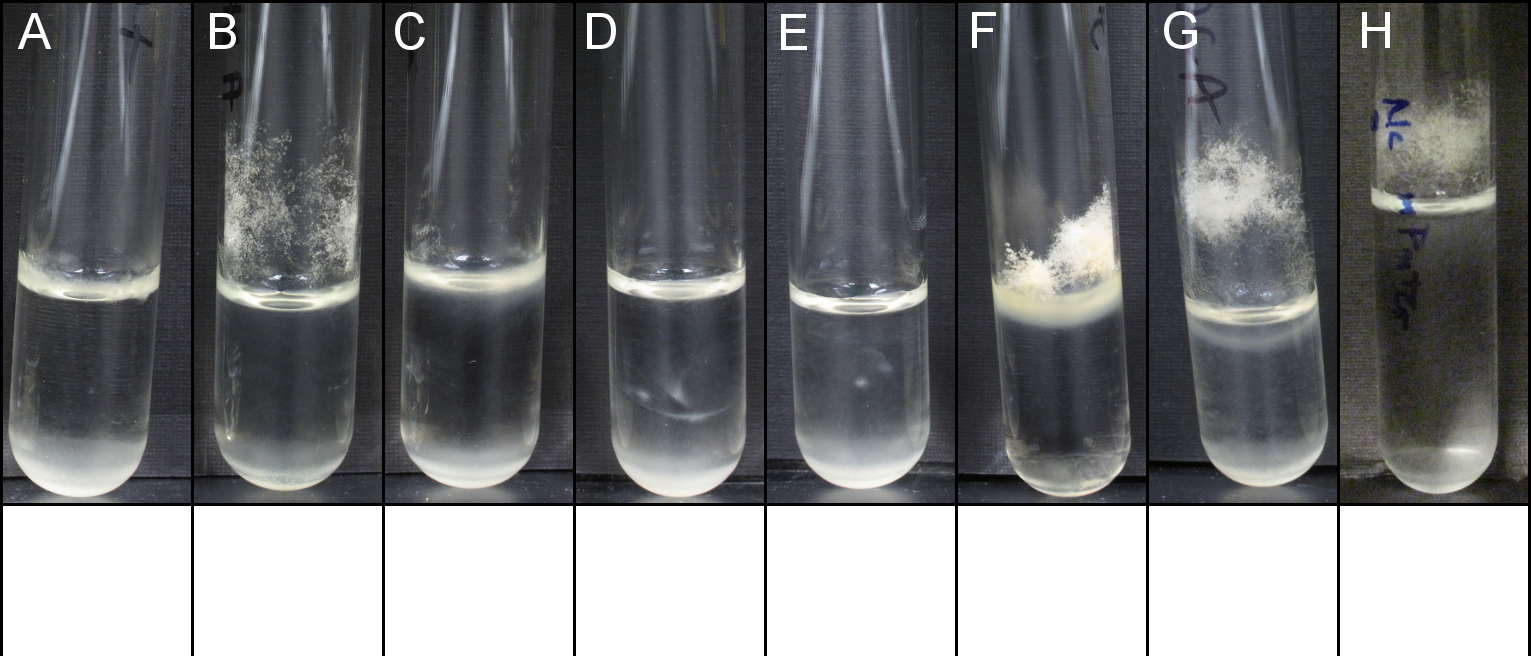
\includegraphics[width=4in]{./Chapter_Inhibition/img/96h_HpNcColdHotFresh.png}
  \caption[Conditioned media inhibits \textit{N. crassa} growth]{Test tubes containing filter-sterilized \textit{Hp}-conditioned media ("filtrate") were inoculated with \textit{N. crassa} conidia and left to incubate at room temperature (~23$^{\circ}$C) for 96h. For A), B), and C), filtrate was derived from initial preparations of \textit{Hp} alone, \textit{N. crassa} alone, and \textit{Hp}+\textit{N. crassa}, respectively. Panel B) establishes that nutrient limitation is not responsible for inhibitory observation as growth of \textit{N. crassa} can still be supported, while A) and C) establish that \textit{Hp} is not exhibiting this behavior as a response to the presence of another fungus. D), E), F), G) contain \textit{Hp}-derived mPmTG filtrate after low (-20$^{\circ}$C), high (60$^{\circ}$C), ultra-low (-80$^{\circ}$) and ultra-high (90$^{\circ}$) temperature treatments, respectively. For D-G, N. crassa inoculation occurred after media was allowed to return to room temperature. H) \textit{N. crassa} growth in fresh mPmTG media.}
  \label{fig:ChInhib_FilterTempAssay}
\end{figure}

\begin{figure}[hb]
  \centering
  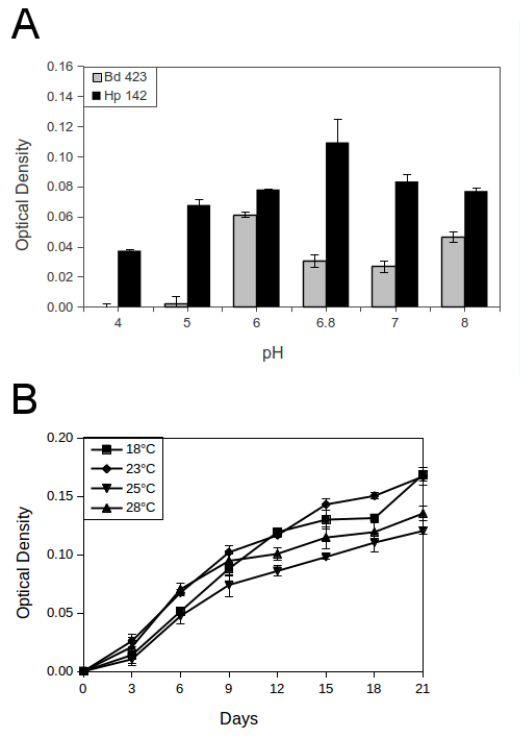
\includegraphics[width=4in]{./Chapter_Inhibition/img/HpBd_pHTempAssay.png}
  \caption[\textit{Hp} is more tolerant of environmental stresses than \textit{Bd}]{A) \textit{Hp} and \textit{Bd} were grown at different pH levels, ranging from 4 to 8. A pH of 6.8 represents the standard pH at which the respective optimal media is prepared. B) \textit{Hp} growth after 21 days at various temperatures ranging from 18$^{\circ}$C to 28$^{\circ}$C.}
  \label{fig:ChInhib_HpBdpHTemp}
\end{figure}

\begin{figure}[hb]
  \centering
  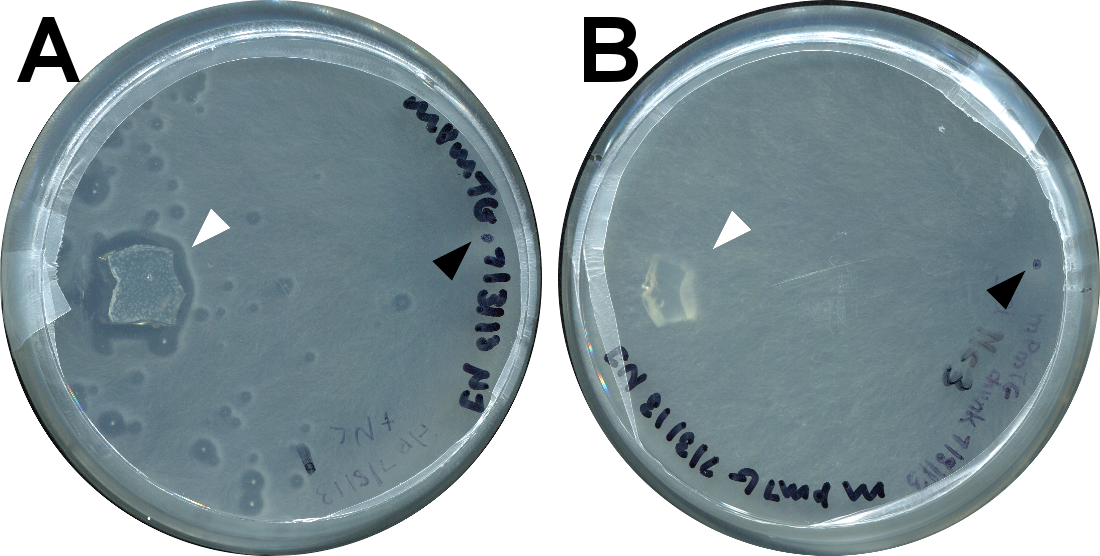
\includegraphics[width=4in]{./Chapter_Inhibition/img/HpNc_avoidance.png}
  \caption[\textit{N. crassa} displays no avoidance behavior of solid agar blocks.]{Solid agar plates of mPmTG media containing A) actively growing \textit{H. polyrhiza} and B) no \textit{H. polyrhiza} growth. After 72 hours post-inoculation of \textit{N. crassa}, zones of inhibition are clearly visible surrounding \textit{H. polyrhiza} sporangia. White arrowheads in A and B indicate agar blocks containing or lacking, respectively, \textit{H. polyrhiza} sporangia. Black arrowheads indicate point of inoculation with \textit{N. crassa} conidia. Plates are 100mm in diameter.}
  \label{fig:ChInhib_NcAvoidance}
\end{figure}

\begin{figure}[hb]
  \centering
  \includegraphics[width=4in]{./Chapter_Inhibition/img/Liquid_Dilution.png}
  \caption[VM dilution series demonstrates efficacy at various concentrations]{VM media diluted with various additives: A) \textit{Hp} filtrate, B) fresh mPmTG, C) \textit{Bd} filtrate, D) fresh 1\% Tryptone. Dilution series in all panels (left to right): 0\% (pure VM), 10\%, 25\%, 50\%, 75\%, 90\%, 100\% (pure additive).}
  \label{fig:ChInhib_LiquidDilution}
\end{figure}

\begin{figure}[hb]
  \centering
  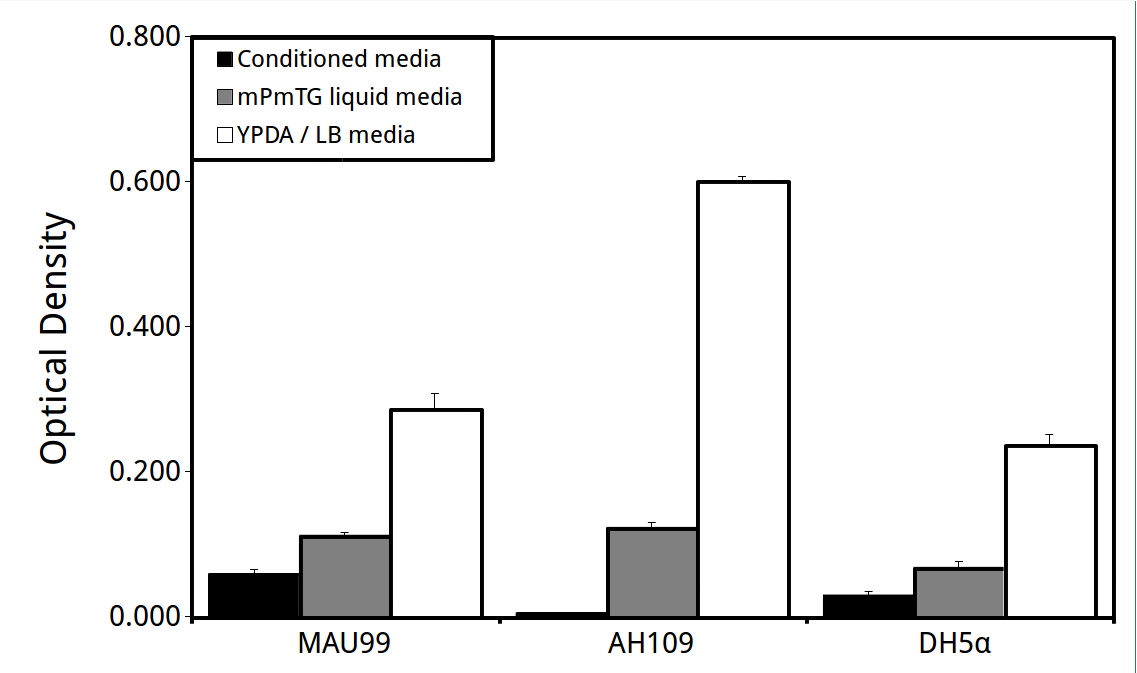
\includegraphics[width=4in]{./Chapter_Inhibition/img/yeastEcoli_liqGrowth.png}
  \caption[\textit{S. cerevisiae} and \textit{E. coli} are inhibited by \textit{Hp} filtrate]{OD$_{600}$ measurements of liquid cultures of \textit{S. cerevisiae} MAU99 and AH109, and \textit{E. coli} DH5$\alpha$ after 72h stationary incubation in different media preparations at room temperature: filter-sterilized \textit{Hp}-conditioned media (black), \textit{Hp} liquid mPmTG media (grey), and either liquid YPDA or LB for yeast or \textit{E. coli}, respectively (white).}
  \label{fig:ChInhib_HpYeastEcoli}
\end{figure}

%%%%%%%%%%%%%%%%%%%%%%%%%%%%%%%%%%%%%%%%%%%%%%%%%%%%%%%%%%%%%%%%%%%%%%%
%% Document: Thesis for PhD at UC Riverside                          %%
%% Description: A comparative analysis of environment sensing in EDF %%
%% Author: Steven Ahrendt                                            %%
%%%%%%%%%%%%%%%%%%%%%%%%%%%%%%%%%%%%%%%%%%%%%%%%%%%%%%%%%%%%%%%%%%%%%%%
% INHIBITION TABLES %
%%%%%%%%%%%%%%%%%%%%%

% Kinase Mutant Screen
% latex table generated in R 3.0.1 by xtable 1.7-4 package
% Sun May 24 12:52:01 2015
\begin{table}[ht]
\centering
\caption{Kinase and phosphotase mutants used in screening against \textit{H. polyrhiza} sporangia.} 
\label{tab:ChInhib_Kinase}
\begin{tabular}{lllll}
  \hline
Mutant & Group & Family & NCU & Neurospora\_gene \\ 
  \hline
x1 & pp2A & - & - & - \\ 
  x2 & ppt-1 & - & - & - \\ 
  x3 & CMGC & MAPK & NCU07024 & os-2 \\ 
  x4 & STE & STE11 & NCU03071 & os-4 \\ 
  x5 & STE & STE7 & NCU00587 & os-5 \\ 
  1846 & CAMK & CAMKL & NCU00914 & stk-16 \\ 
  1849 & Other & PEK & NCU01187 & cpc-3 \\ 
  1885 & STE & STE20 & NCU03894 & stk-4 \\ 
  1888 & Other & WEE & NCU04326 & stk-29 \\ 
  1916 & Unclassified & - & NCU06421 & stk-41 \\ 
  1917 & Unclassified & - & NCU06422 & stk-42 \\ 
  1919 & Unclassified & - & NCU06583 & stk-44 \\ 
  1920 & Other & VPS15 & NCU06626 & stk-45 \\ 
  1925 & AGC & YANK & NCU07062 & stk-49 \\ 
  1936 & CGMC & CLK/SRPK & NCU10004 & stk-56 \\ 
  1937 & Unclassified & - & NCU05638 & stk-34 \\ 
  1944 & CMGC & CDK & NCU07880 & prk-6 \\ 
  1946 & Other & IKS & NCU08177 & stk-51 \\ 
  2294 & CAMK & CAMKL & NCU04747 & stk-31 \\ 
   \hline
\end{tabular}
\end{table}
% Chytrid secretome
% latex table generated in R 3.0.1 by xtable 1.7-4 package
% Sun May 24 12:52:01 2015
\begin{table}[ht]
\centering
\caption[Chytrid secretome predictions]{Proteins predicted to be in the secretome of basal fungi} 
\label{tab:ChInhib_ChySec}
\begin{tabular}{rr}
  \hline
 & Num of proteins \\ 
  \hline
R. allomycis &  32 \\ 
  G. prolifera & 101 \\ 
  Piromyces E2 & 269 \\ 
  Orpinomyces C1 & 280 \\ 
  H. polyrhiza &  58 \\ 
  S. punctatus &  66 \\ 
  B. dendrobatidis & 133 \\ 
  A. macrogynus &  57 \\ 
  C. anguillulae & 101 \\ 
  C. lativittatus &  98 \\ 
   \hline
\end{tabular}
\end{table}

%%%%%%%%%%%%%%%
% CONCLUSIONS %
%%%%%%%%%%%%%%%
%%%%%%%%%%%%%%%%%%%%%%%%%%%%%%%%%%%%%%%%%%%%%%%%%%%%%%%%%%%%%%%%%%%%%%%%%%%%%%%%%
%% Document: Thesis for PhD at UC Riverside                                    %%
%% Title: Investigating the evolution of environmental and biotic interactions %%
%%          in basal fungal lineages through comparative genomics              %%
%% Author: Steven Ahrendt                                                      %%
%%%%%%%%%%%%%%%%%%%%%%%%%%%%%%%%%%%%%%%%%%%%%%%%%%%%%%%%%%%%%%%%%%%%%%%%%%%%%%%%%
% CONCLUSIONS %
%%%%%%%%%%%%%%%
\chapter{Conclusions}
The objective of this dissertation research was to enhance the current knowledge about basal fungal groups. Genomic resources and methodologies are becoming increasingly more accessible, and so the ability to incorporate this data into existing studies is becoming more widespread.\\
\indent This objective was addressed through the following specific aims:\\
\begin{enumerate}
  \item Describe and identify a compopund responsible for antifungal behavior (Chapter~\ref{chap:HpInhibition})
  \item Characterize the identification of an opsin-like protein, through both structural analyses (Chapter~\ref{chap:RhodStruct}) as well as accessory and downstream proteins (Chapter~\ref{chap:RhodAux})
  \item Produce and interpret a transcriptome for mosquito pathogen, thereby laying groundwork for enhanced genomic resources for this organism (Chapter~\ref{chap:ClatTranscriptome})
\end{enumerate}
\section{Inhibitory properties of \textit{Homolaphlyctis polyrhiza}}
In 1854, Louis Pasteur commented that "In the fields of observation, chance favors only the prepared mind." My surprising and unexpected observation in the Stajich lab of the non-pathogenic Chytridiomycte isolate \textit{Homolaphlyctis polyrhiza} JEL142 inhibiting vegetative hyphal growth of a \textit{Neurospora crassa} contaminant prompted an investigation into its biological nature. My work for this investigation pursued three major questions: "Is this a unique property of \textit{Hp}?", "Is this a specific interaction with \textit{N. crassa}?", and "What is the chemical nature of the responsible compound?"\\
\indent By examining five other chytrid species in culture, I have evidence supporting the idea that this is a specific behavior for \textit{Hp}. No other chytrid surveyed displayed the appropriate inhibitory phenotype, including the most closely related chytrid to \textit{Hp}, the amphibian pathogen \textit{Batrachochytrium dendrobatidis}.\\
\indent Next, I expanded the potential targets of \textit{Hp} to include members of the Ascomycota, Basidiomycota, and Zygomycota. All of these targets were susceptible to \textit{Hp}, with the exception of \textit{Rhizopus oryzae}.\\
\indent Finally, I looked for the chemical nature for the mechanism of action by liquid assay and computational screening. I determined that the active compound is soluble and stable for at least 96h absent any \textit{Hp} sporangia. Additionally, liquid obtained from preparations featuring both \textit{Hp}+\textit{N. crassa} and \textit{Hp} alone were indistinguishably effective against reintroduction of \textit{N. crassa} conidia.\\
\indent Taken together, these data suggest that the compound is a constitutively-produced secondary metabolite compound with broadly specific activity. Its mechanism of action is unknown, as are its chemical structure and related biosynthetic pathway(s). Near term future work will necessarily focus on chemical profiling of bioactive spent media filtrate to generate a working hypothesis for the chemical nature of the product. A starting point for this research is provided in the form of \textit{in silico} genomic and transcriptomic research. Finally, it is worth noting that the relative ease with which this discovery was made speaks to the necessity for further research into these basal lineages, of which intimate genomic and biochemical knowledge is lacking.\\
\section{Structural mechanics and components of basal fungal rhodopsin photosensory pathways}
Sunlight is one of the most obvious environmental sources of information, and the most easily studied. It should come as no surprise that photoreception exists in some form in all three domains of life, however varied in its implementation. The research in Chapters~\ref{chap:RhodStruct} and \ref{chap:RhodAux} address four key questions: "How similar, structurally, are the opsin-like proteins from chytrids to each other and to other experimentally verified photoreceptors?", "How does this structural similarity (or dissimilarity) impact functional photoreception?", "What is the complement of downstream associated compenents (eg heterotrimeric G-protein subunits)?", and "Do the auxilary protein presence/absence correlate with known aspects of the evolution of photobiology in fungi?" \\
\indent Sequence homology predicts a number of seven-transmembrane domain proteins in various chytrid species, with particular similarity to the members of the Type 2 GPCR rhodopsin family. I used sequences from \textit{B. dendrobatidis}, \textit{S. punctatus}, and \textit{A. macrogynus} in homology modeling against known rhodopsin crystal structures to produce 3D structural models of these "chytriopsins". Quality metrics indicate that these computational models are reasonably sound predictions of the protein structures as they exist in the cell.\\
\indent Therefore they are good candidates for analysis in ligand docking and molecular dynamics simulations to infer biological function. The structural analysis suggests that the rhodopsin-like protein identified in \textit{S. punctatus} is most likely to be functional given the conservation of important structural features, most importantly the conserved lysine residue to which the chromophore ligand is bound. Automated non-covalent docking screens of retinal-like ligands against other chytropsin proteins from \textit{B. dendrobatidis} and \textit{A. macrogynus} suggest that even though these proteins lack the conserved lysine in a proper position, the binding pockets are spatially and chemically able to accomodate the 11-\textit{cis}-retinal chromophore.\\
\indent Covalent docking prediction of the \textit{Sp} protein using 11-\textit{cis}-retinal suggests that it is the most likely to be functionally active. This prediction was further refined with MD simulations using AMBER. The results were compared to the experimentally verified interaction between the \textit{Todares pacificus} rhodopsin and 11-\textit{cis}-retinal (PDB ID: 2Z73). \\
\section{Transcriptome analysis of the entomopathogenic Blastocladiomycete \textit{Coelomomyces lativittatus}}
Species in the basal fungal lineages occupy a diverse collection of environmental niches, including symbionts, pathogens, and saprotrophs. However, species in the genus \textit{Coelomomyces}, itself a member of the Blastocladiomycota, are the only known basal fungi which are pathogenic in arthropods. Specifically, their development requires oscillation between two hosts: mosquito larvae and microcrustaceans. This lifecycle has made them both attractive targets for research into non-pesticide-based mosquito control, yet also difficult systems in which to pursue this research. The transcriptome analysis presented in Chapter~\ref{ClatTranscriptome} was addressing two major points about entompathogenic chytrids, using \textit{Coelomomyces lativittatus} as a model: "How do aspects of the transcriptome regarding already known aspects of \textit{C. lativittatus} biology, specifically regarding $\beta$-carotene biosynthesis, environment sensing, and insect-association?", and "How does the protein complement of \textit{C. lativittatus} compare related Chytridiomycete and Blastocladiomycete species which are not insect-associated?"\\
\indent PFAM prediction suggests a number of candidate enzymes related to insect virulence, the most prominent being members of the C1 peptidase family. These have documented antihelmintic effects and cuticle degrading activity in nematodes. Furthermore, this family seems expanded in \textit{C. lativittatus} relative to other basal fungi, which are not insect-associated organisms.\\
\indent The transcriptome analysis demonstrated that \textit{C. lativittatus} likely has a complete complement of $\beta$-carotene processing enzymes, despite the apparent lack of one enzyme in the pathway: phytoene desaturase, the first enzyme in the three step cascade and responsible for converting phytoene to lycopene. Because the other two enzymes are accounted for, and because \textit{Coelomomyces} are experimentally verified producers of $\beta$-carotene, it is unlikely that there is a novel biosynthetic pathway at work and instead the phyotene desaturase mRNA was not expressed at a high enough level to be recovered in either RNA extraction or during the HT sequencing.\\ 
\indent The descriptive results from this investigation serve as starting points for future work involving genomic, transcriptomic, and proteomic analyses from multiple developmental stages and timepoints.\\



%%%%%%%%%%%%%%%%
% BIBLIOGRAPHY %
%%%%%%%%%%%%%%%%
%\nocite{*}
% \singlespacing
%\bibliographystyle{alpha} % Alphabetical 
%\bibliographystyle{plain} % default in UCR template
\bibliographystyle{ieeetr} % this style lists refs in order of appearance
\bibliography{Ahrendt_thesisRefs}

%%%%%%%%%%%%
% APPENDIX %
%%%%%%%%%%%%
\appendix
%%%%%%%%%%%%%%%%%%%%%%%%%%%%%%%%%%%%%%%%%%%%%%%%%%%%%%%%%%%%%%%%%%%%%%%%%%%%%%%%%
%% Document: Thesis for PhD at UC Riverside                                    %%
%% Title: Investigating the evolution of environmental and biotic interactions %%
%%          in basal fungal lineages through comparative genomics              %%
%% Author: Steven Ahrendt                                                      %%
%%%%%%%%%%%%%%%%%%%%%%%%%%%%%%%%%%%%%%%%%%%%%%%%%%%%%%%%%%%%%%%%%%%%%%%%%%%%%%%%%
%% FLAGELLAR ANALYSIS %
%%%%%%%%%%%%%%%%%%%%%%%
\chapter{Comparative genomics analysis of Flagellar motility}
\label{app:Flagella}
\section{Introduction}
The eukaryotic flagellum is a protenaceous structure which provides motility to single-celled organisms [citation needed]. In fungi, only members of the basal lineages (specifically the Cryptomycota, Chytridiomycota, Blastocladiomycota, and Neocallimastigomycota) posess a flagellum and motile zoosporic life stage. Members of the Glomeromycota, Basidiomycota, and Ascomycota do not have such a life stage [citation needed] and are commonly considered "terrestrial fungi". Notable exceptions to this pattern include the Microsporidian lineage, which is considered a member of the basal fungi but whose members are not flagellated, and \textit{Olpidium brassicae}, a flagellated, single-celled organism morphologically similar to other chytrids but phylogenetically similar to terrestrial fungi \cite{Sekimoto2011}. \\
\section{Results and Discussion}
A search for Rozella homologs of flagellar-associated proteins from the \textit{Naeglaria} genome \cite{FritzLaylin2011} reveal a pattern of presence/absence of proteins in Rozella which correlates with that found in the Chytridiomycota and Blastocladiomycota. This pattern, in general, differs from the Microsporidia, supporting the placement of Rozella as prior to the Chytridiomycota/Blastocladiomycota and a flagellar loss event after the divergence of the Microsporidia. \\
\indent The heatmap displayed in Figure~\ref{fig:AppFlag_heatmap} indicates presence or absence of proteins in the \textit{Naeglaria} dataset as identified in the proteomes of other fungi searched. By clustering based on presence/absence patterns, the flagellated vs non-flagellated organisms separate into distinct groups consistent with known phylogeny (ie basal lineages separate from Dikarya and Zygomycetes). It's possible to collect a subset of genes which are present in basal (flagellated) lineages and absent in terrestrial (non-flagellated) lineages. Presumably, these have more pronounced association with flagellar assembly and function. Furthermore, take the subset of proteins present in all lineages and do pairwise distance alignment to see if, while being from the same family / hits to same query, these genes mutated or transititioned to new structures / functionalities over evolutionary time.\\
\section{Methods}
The flagellar analysis was carried out using a dataset of 173 flagellar motility proteins obtained from the \textit{Naeglaria grubeii} genome sequence \cite{FritzLaylin2011}. These proteins were used in a FASTA search (SSEARCH v36.07) using an e-val cutoff of e-20. Heatmap generation was accomplished using $pheatmap()$ in R.\\
\indent Multiple sequence alignment and distance matrix generation was performed on the subset of genes present in all organisms using $tcoffee$ and $phylip$.\\

%%%%%%%%%%%%%%%%%%%%%%%
%% Document: Thesis for PhD at UC Riverside
%% Title: Investigating 
%% Author: Steven Ahrendt
%%%%%%%%%%%%%%%%%%%%%%%%%%%%%%%%%%%%%%
% APPENDIX FIGURES %
%%%%%%%%%%%%%%%%%%%%

% Flagellar heat map from James et al 2009
\begin{figure}
\begin{center}
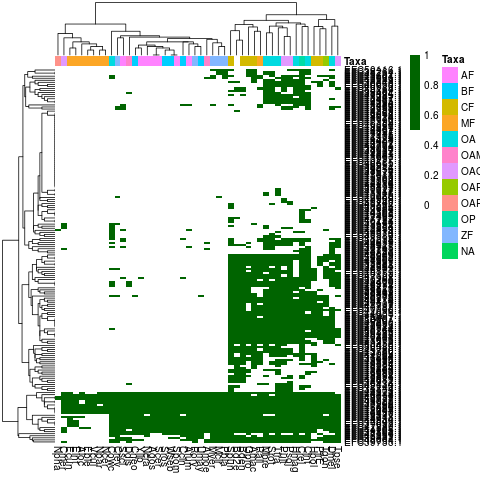
\includegraphics{./Appendix/img/heatmap.png}
\end{center}
\caption[Heatmap cluster analysis of flagellar proteins from \textit{Naegleria gruberi}]{Protein copies identified in proteomes of interest are normalized to indicate presence and absence only, where green indicates that one or more copies were found. Proteins are listed on the right, and proteomes given on the bottom. Both rows and columns are clustered by the "complete" method}
\label{fig:AppFlag_heatmap}
\end{figure}

%%%%%%%%%%%%%%%%%%%%%%%%%%%%%%%%%%%%%%%%%%%%%%%%%%%%%%%%%%%%%%%%%%%%%%%%%%%%%%%%%
%% Document: Thesis for PhD at UC Riverside                                    %%
%% Title: Investigating the evolution of environmental and biotic interactions %%
%%          in basal fungal lineages through comparative genomics              %%
%% Author: Steven Ahrendt                                                      %%
%%%%%%%%%%%%%%%%%%%%%%%%%%%%%%%%%%%%%%%%%%%%%%%%%%%%%%%%%%%%%%%%%%%%%%%%%%%%%%%%%
%% MISC DATA USED IN THESIS %
%%%%%%%%%%%%%%%%%%%%%%%%%%%%%
\chapter{Datasets and scripts}
\label{app:Data}
\section{Datasets}
\begin{itemize}
  \item List of proteomes from each organisms, the source website, and version used in these analyses is provided in Table~\ref{tab:AppData_taxa}.\\
  \item PDB IDs used in the structural modeling, docking, and MD simulations presented in Chapter~\ref{chap:RhodStruct} are provided in Table~\ref{tab:AppData_PDB}.\\
\end{itemize}
\section{Scripts}
All scripts are available on github.

%%%%%%%%%%%%%%%%%%%%%%%%%%%%%%%%%%%%%%%%%%%%%%%%%%%%%%%%%%%%%%%%%%%%%%%
%% Document: Thesis for PhD at UC Riverside                          %%
%% Description: A comparative analysis of environment sensing in EDF %%
%% Author: Steven Ahrendt                                            %%
%%%%%%%%%%%%%%%%%%%%%%%%%%%%%%%%%%%%%%%%%%%%%%%%%%%%%%%%%%%%%%%%%%%%%%%
% MISC LIST OF DATA %
%%%%%%%%%%%%%%%%%%%%%

% Taxa and sources
% latex table generated in R 3.0.1 by xtable 1.7-4 package
% Sat May 23 12:26:50 2015
\centering
{\renewcommand{\arraystretch}{0.5}
{\footnotesize
{\setlength{\tabcolsep}{1pt}
\begin{longtable}{rllrlll}
\caption[List of proteomes used in comparative analyses.]{List of all proteomes used in comparative analyses, including NCBI taxonomy database ID, phylogenetic group abbreviation ("Class2"), phylum designation ("Class1"), isolate number/version (where applicable), and source website.} \label{tab:AppData_taxa} \\
  \hline
\hline
 & Class2 & Class1 & TaxID & Name & Isolate/Version & Source \\ 
  \hline
Aben & APF & Ascomycota & 663331 & Arthroderma benhamiae & CBS 112371 & \cite{Aben} \\ 
  Afum & AEF & Ascomycota & 746128 & Aspergillus fumigatus & Af293 & \cite{Afum} \\ 
  Agos & ASaF & Ascomycota & 33169 & Ashbya gossypii & --- & \cite{Agos} \\ 
  Aloc & MF & Microsporidia & 278021 & Antonospora locustae & --- & \cite{Aloc} \\ 
  Amac & CBF & Chytrids & 28583 & Allomyces macrogynus & ATCC 38327 & \cite{Amac} \\ 
  Amoe & OAM & Amoebozoa & 1243176 & Amoeboaphelidium & --- & \cite{Amoe} \\ 
  Anid & AEF & Ascomycota & 227321 & Aspergillus nidulans & FGSC A4 & \cite{Anid} \\ 
  Bcin & ALoF & Ascomycota & 332648 & Botrytis cinerea & B05.10 & \cite{Bcin} \\ 
  Bcir & ZMF & Zygomycota & 1314798 & Backusella circina & FSU 941 & \cite{Bcir} \\ 
  Bden & CCF & Chytrids & 109871 & Batrachochytrium dendrobatidis & JEL 423 & \cite{Bden} \\ 
  Bder & AEF & Ascomycota & 559298 & Blastomyces dermatitidis & SLH14081 & \cite{Bder} \\ 
  Beme & CBF & Chytrids & 4808 & Blastocladiella emersonii & --- & \cite{Beme} \\ 
  Cang & CBF & Chytrids & 109876 & Catenaria anguillulae & --- & \cite{Cang} \\ 
  Ccin & BAF & Basidiomycota & 5346 & Coprinopsis cinerea & --- & \cite{Ccin} \\ 
  Ccor & ZEF & Zygomycota & 34488 & Conidiobolus coronatus & --- & \cite{Ccor} \\ 
  Cimm & AEF & Ascomycota & 246410 & Coccidioides immitis & RS & \cite{Cimm} \\ 
  Cint & OA & Animal & 7719 & Ciona intestinalis & --- & \cite{Cint} \\ 
  Clat & CBF & Chytrids & 945690 & Coelomomyces lativittatus & --- & \cite{Clat} \\ 
  Cmer & OAO & OAO & 45157 & Cyanidioschyzon merolae & --- & \cite{Cmer} \\ 
  Cneo & BAF & Basidiomycota & 5207 & Cryptococcus neoformans & H99 & \cite{Cneo} \\ 
  Cowc & OA & Animal & 192875 & Capsaspora owczarzaki & ATCC 30864 & \cite{Cowc} \\ 
  Crei & OP & Plant & 3055 & Chlamydomonas reinhardtii & --- & \cite{Crei} \\ 
  Crev & ZF & Zygomycota & 61392 & Coemansia reversa & --- & \cite{Crev} \\ 
  Daci & ADF & Ascomycota & 112489 & Dissoconium aciculare & --- & \cite{Daci} \\ 
  Dbis & BAF & Basidiomycota & 1314803 & Dendrothele bispora & --- & \cite{Dbis} \\ 
  Ddis & OAM & Amoebozoa & 44689 & Dictyostelium discoideum & --- & \cite{Ddis} \\ 
  Dmel & OA & Animal & 7227 & Drosophila melanogaster & --- & \cite{Dmel} \\ 
  Dsym & ADF & Ascomycota & 548649 & Dothidotthia symphoricarpi & --- & \cite{Dsym} \\ 
  Ebie & MF & Microsporidia & 31281 & Enterocytozoon bieneusi & --- & \cite{Ebie} \\ 
  Ecun & MF & Microsporidia & 6035 & Encephalitozoon cuniculi & --- & \cite{Ecun} \\ 
  Eint & MF & Microsporidia & 58839 & Encephalitozoon intestinalis & --- & \cite{Eint} \\ 
  Falb & OAM & Amoebozoa & 691883 & Fonticula alba & ATCC 38817,V2 & \cite{Falb} \\ 
  Fgra & ASoF & Ascomycota & 229533 & Fusarium graminearum  & PH-1 & \cite{Fgra} \\ 
  Gpro & CF & Chytrids & 1123529 & Gonapodya prolifera & --- & \cite{Gpro} \\ 
  Hmag & OA & Animal & 6085 & Hydra magnipapillata & --- & \cite{Hmag} \\ 
  Hpol & CCF & Chytrids & 166479 & Homolaphlyctis polyrhiza & JEL 142 & \cite{Hpol} \\ 
  Hsap & OA & Animal & 9606 & Homo sapiens & --- & \cite{Hsap} \\ 
  Lhya & ZF & Zygomycota & 420593 & Lichtheimia hyalospora & --- & \cite{Lhya} \\ 
  Lmac & ADF & Ascomycota & 372055 & Lophiostoma macrostomum & --- & \cite{Lmac} \\ 
  Mani & ASoF & Ascomycota & 5530 & Metarhizium anisopliae & --- & \cite{Mani} \\ 
  Mbre & OA & Animal & 81824 & Monosiga brevicollis & MX1 & \cite{Mbre} \\ 
  Mcan & AEF & Ascomycota & 554155 & Microsporum canis & CBS 113480 & \cite{Mcan} \\ 
  Mcir & ZMF & Zygomycota & 36080 & Mucor circinelloides & --- & \cite{Mcir} \\ 
  Mmus & OA & Animal & 10090 & Mus musculus & --- & \cite{Mmus} \\ 
  Mver & ZMF & Zygomycota & 78898 & Mortierella verticillata & NRRL 6337 & \cite{Mver} \\ 
  Ncer & MF & Microsporidia & 40302 & Nosema ceranae & --- & \cite{Ncer} \\ 
  Ncra & ASoF & Ascomycota & 5141 & Neurospora crassa & --- & \cite{Ncra} \\ 
  Npar & MF & Microsporidia & 586133 & Nematocida parisii & ERTm1 & \cite{Npar} \\ 
  Npha & OAR & Archaea & 348780 & Natromonas pharaonis & --- & \cite{Npha} \\ 
  OrpC & CNF & Chytrids & 1117330 & Orpinomyces spp & C1A & \cite{OrpC} \\ 
  Patr & ADF & Ascomycota & 703506 & Patellaria atrata & --- & \cite{Patr} \\ 
  Pbla & ZMF & Zygomycota & 4837 & Phycomyces blakesleeanus & NRRL1555,v2.0.JGI & \cite{Pbla} \\ 
  Pgra & BPF & Basidiomycota & 418459 & Puccinia graminis f.sp. tritici & CRL75-36-700-3 & \cite{Pgra} \\ 
  PirE & CNF & Chytrids & 45796 & Piromyces spp  & E2 & \cite{PirE} \\ 
  Psip & ADF & Ascomycota & 100044 & Pleomassaria siparia & --- & \cite{Psip} \\ 
  Psoj & OAO & OAO & 67593 & Phytophthora sojae & --- & \cite{Psoj} \\ 
  Ptri & ADF & Ascomycota & 426418 & Pyrenophora tritici-repentis & Pt-1C-BFP & \cite{Ptri} \\ 
  Pult & OAO & OAO & 431595 & Pythium ultimum & DAOM BR144,v.2010-07-12 & \cite{Pult} \\ 
  Rall & MF & Microsporidia & 281847 & Rozella allomycis & v.2012-05-03 & \cite{Rall} \\ 
  Rdel & ZMF & Zygomycota & 936053 & Rhizopus delemar & --- & \cite{Rdel} \\ 
  Rirr & ZMF & Zygomycota & 588596 & Rhizophagus irregularis & --- & \cite{Rirr} \\ 
  Rmic & ZMF & Zygomycota & 58291 & Rhizopus microsporus var microsporus & v1.0 & \cite{Rmic} \\ 
  Rory & ZMF & Zygomycota & 64495 & Rhizopus oryzae (delamar) & 99-880,v.1 & \cite{Rory} \\ 
  Sarc & OA & Animal & 72019 & Sphaeroforma arctica  & JP610 & \cite{Sarc} \\ 
  Scer & ASaF & Ascomycota & 4932 & Saccharomyces cerevisiae & S288C,v.2011-02-03 & \cite{Scer} \\ 
  Sfim & ADF & Ascomycota & 718229 & Sporormia fimetaria & --- & \cite{Sfim} \\ 
  Spom & ATF & Ascomycota & 4896 & Schizosaccharomyces pombe & v.20 & \cite{Spom} \\ 
  Spun & CCF & Chytrids & 109760 & Spizellomyces punctatus & DAOM BR117 & \cite{Spun} \\ 
  Sros & BF & Basidiomycota & 40563 & Sporobolomyces roseus & --- & \cite{Sros} \\ 
  Srot & OA & Animal & 946362 & Salpingoeca rosetta & --- & \cite{Srot} \\ 
  Sscl & ALoF & Ascomycota & 665079 & Sclerotinia sclerotiorum & 1980\_UF-70.30,v.2009-01.Broad & \cite{Sscl} \\ 
  Tgon & OAP & Apicomplexian & 5811 & Toxoplasma gondii & ME49,v.2008-07-23.ToxoDB-7.2 & \cite{Tgon} \\ 
  Tpse & OAO & OAO & 35128 & Thalassiosira pseudonana & CCMP1335,v.JGI3 & \cite{Tpse} \\ 
  Trub & AEF & Ascomycota & 559305 & Trichophyton rubrum & CBS 118892 & \cite{Trub} \\ 
  Ttra & OA & Animal & 529818 & Thecamonas trahens & ATCC 50062 & \cite{Ttra} \\ 
  Umay & BUF & Basidiomycota & 5270 & Ustilago maydis & v.2011-05-24.MIPS & \cite{Umay} \\ 
  Uram & ZMF & Zygomycota & 41833 & Umbelopsis ramanniana & --- & \cite{Uram} \\ 
  Uree & AEF & Ascomycota & 336963 & Uncinocarpus reesii & UAMH 1704 & \cite{Uree} \\ 
  Vcul & MF & Microsporidia & 103449 & Vavraia culicis floridensis & v.1.Broad & \cite{Vcul} \\ 
  Wseb & BAF & Basidiomycota & 148960 & Wallemia sebi & CBS-633.66,v.JGI1 & \cite{Wseb} \\ 
  Ylip & ASaF & Ascomycota & 4952 & Yarrowia lipolytica & CLIB122,v.14-APR-2010 & \cite{Ylip} \\ 
  Zrhi & ADF & Ascomycota & 1314779 & Zopfia rhizophilia & CBS 207.26,v1.0 & \cite{Zrhi} \\ 
   \hline
\hline
\end{longtable}
} %horizontal spacing
} %footnote size
} %vertical spacing
% PDB IDs
% latex table generated in R 3.0.1 by xtable 1.7-4 package
% Sat May 23 12:26:50 2015
\begin{table}[h]
\centering
\caption[PDB IDs and descriptions of structures used in comparative analyses]{PDB IDs and descriptions of structures used in docking and Molecular dynamics simulations} 
\label{tab:AppData_PDB}
\begin{tabular}{rll}
  \hline
\hline
 & PDBID & Description \\ 
  \hline
1 & 1U19 & Crystal structure of Bovine rhodopsin at 2.2 angstroms resolution \\ 
  2 & 2Z73 & Crystal structure of Squid rhodopsin \\ 
  3 & 1H68 & Sensory rhodopsin II \\ 
   \hline
\hline
\end{tabular}
\end{table}

\end{document}
